%%% The main file. It contains definitions of basic parameters and includes all other parts.


%% Settings for two-sided (duplex) printing
\documentclass[10pt,a4paper]{report}
\let\openright=\cleardoublepage

%% Character encoding: usually latin2, cp1250 or utf8:
\usepackage[utf8]{inputenc}

%% It's 2019
\usepackage[default]{droidserif}
\usepackage[T1]{fontenc}

%% Further useful packages (included in most LaTeX distributions)
\usepackage{amsmath}        % extensions for typesetting of math
\usepackage{amsfonts}       % math fonts
\usepackage{graphicx}       % embedding of pictures
\usepackage{tikz}
%\usetikzlibrary{shapes,fit,positioning,snakes,mindmap,trees,decorations.text,arrows.meta}
%\makenomenclature
\usepackage{algorithm,algpseudocode}
\usepackage{booktabs}
\usepackage{mwe}
\usepackage{afterpage}
\usepackage{pgfgantt}
\usepackage{pdflscape}
\usepackage{geometry}
\usepackage{enumitem}
\usepackage{float}
\usepackage{framed}
\usepackage{titlesec}
\usepackage{listings}
\usepackage{xcolor}
\usepackage{longtable}
\usepackage{makecell}
\usepackage[toc,page]{appendix}
\usepackage{multirow}
\usepackage{tocbibind}
\usepackage{etoolbox}
\usepackage{fancyvrb}

\lstset{basicstyle=\ttfamily,
	showstringspaces=false,
	commentstyle=\color{red},
	keywordstyle=\color{blue}
}

\usepackage{pdfpages}

\usepackage[textsize=tiny,backgroundcolor=yellow!50, linecolor=black!25]{todonotes}

% links shall be clickable
\usepackage[unicode]{hyperref}   % Must follow all other packages
\usepackage{cleveref} % Must follow all other packages including hyperref
\AtBeginEnvironment{appendices}{\crefalias{chapter}{appendix}}

% indexing
\usepackage{makeidx}
\makeindex
\usepackage[totoc, columns=1]{idxlayout}
% Definitions of macros (see description inside)

\newcommand{\cool}{\color{green!50!white!80!black}}
\newcommand{\textcool}[1]{{\cool #1}}

\newcommand{\XX}[1]{\textcolor{red}{#1}}
\newcommand{\TT}[1]{\texttt{#1}}
\newcommand{\SC}[1]{{\fontfamily{phv}\selectfont\textsc{#1}}}

% Draw black "slugs" whenever a line overflows, so that we can spot it easily.


% avoid some slugs naturally
\clubpenalty=1000
\widowpenalty=1000
%\hyphenpenalty=100  % turn this on to prevent hyphenation
\emergencystretch=2cm


%%% The field of all real and natural numbers
\newcommand{\R}{\mathbb{R}}
\newcommand{\N}{\mathbb{N}}
\newcommand{\F}{\mathbb{F}}
\newcommand{\Z}{\mathbb{Z}}

\newcommand{\bms}{\begin{enumerate}[label=\bf (M\arabic*)]}
\newcommand{\bwp}{\begin{enumerate}[label=\bf \normalsize  (WP\arabic*), resume=del]}
\newcommand{\eenum}{\end{enumerate}}
\newcommand{\itemm}{\large \item }
\newcommand{\itemwp}{ \normalsize \item }
\newcommand{\deadline}[2]{\small (deadline: \textit{month #1}, duration: \textit{#2 moths})}
\newcommand{\people}[1]{\textit{\small (#1)}}


% move the headings out of gutenberg era
\setcounter{secnumdepth}{4}
\titleformat{\chapter}{\cool\fontsize{24pt}{24pt}\bfseries}{\color{black!25}\thechapter.}{1em}{}
\titleformat{\section}{\cool\fontsize{16pt}{18pt}\bfseries}{\scriptsize\color{black!25}\thesection}{1em}{}
\titleformat{\subsection}{\cool\fontsize{12pt}{14pt}\bfseries}{\scriptsize\color{black!25}\thesubsection}{1em}{}
\titleformat{\subsubsection}{\cool\bfseries}{\scriptsize\color{black!25}\thesubsubsection}{1em}{}

% code floats
\colorlet{shadecolor}{cyan!10}
\makeatletter
\newcommand\floatc@code[2]{{\@fs@cfont #1} #2\par}
\newcommand\fs@code{\def\@fs@cfont{\bfseries}\let\@fs@capt\floatc@code
\def\@fs@pre{}%
\def\@fs@mid{\vspace{-.5ex}\begin{shaded}}%
\def\@fs@post{\vspace{-1em}\end{shaded}}%
\let\@fs@iftopcapt\iftrue}
\makeatother

\floatstyle{code}
\newfloat{listing}{tbp}{lst}
\floatname{listing}{Listing}

% file indexing
\makeatletter
\def\patheach#1#2#3{\@test@patheachF{#1}{#2}#3/\endgroup}
\def\@test@patheachF#1#2#3\endgroup{\if#3\empty\empty\else\@patheachF{#1}{#2}#3\endgroup\fi}
\def\@patheachF#1#2#3/{#1{#3}\@test@patheach{#1}{#2}}
\def\@test@patheach#1#2#3\endgroup{\if#3\empty\empty\else\@patheach{#1}{#2}#3\endgroup\fi}
\def\@patheach#1#2#3/{#2#1{#3}\@test@patheach{#1}{#2}}
\def\foreach#1#2{\@test@foreach{#1}#2,\endgroup}
\def\@test@foreach#1#2\endgroup{\if#2\empty\empty\else\@foreach{#1}#2\endgroup\fi}
\def\@foreach#1#2,{#1{#2}\@test@foreach{#1}}
\makeatother

\def\makefileindex#1{%
\index{\patheach{\texttt}{!}{#1}}%
\hspace{-1ex}\texttt{\patheach{}{/\-}{#1}}\\}

\def\makefileindexnotext#1{%
	\index{\patheach{\texttt}{!}{#1}}}

\def\makefileindexes#1{\foreach{\makefileindex}{#1}}

\newcommand{\srcstyle}[1]{\tt\scriptsize\textcolor{gray}{\makefileindexes{#1}}}
\newcommand{\sectionFiles}[2]{ \strut~\hfill~\hspace{1ex}~\parbox{#1}{\tt\scriptsize\textcolor{gray}{\makefileindexes{#2}}}}

\newcommand{\chapterSrc}[3][.4\linewidth]{\chapter[#2]{#2\sectionFiles{#1}{#3}}}
\newcommand{\sectionSrc}[3][.4\linewidth]{\section[#2]{#2\sectionFiles{#1}{#3}}}
\newcommand{\subsectionSrc}[3][.4\linewidth]{\subsection[#2]{#2\sectionFiles{#1}{#3}}}
\newcommand{\subsubsectionSrc}[3][.4\linewidth]{\subsubsection[#2]{#2\sectionFiles{#1}{#3}}}

% index typesetting customization
\renewcommand\indexname{Source file documentation index}
\providecommand*\lettergroup[1]{}
\makeatletter
\newcommand\idxitem{\@idxitem}
\newcommand\idxIitem{\@idxitem\texttt{.\ }}
\newcommand\idxIIitem{\@idxitem\texttt{.\ .\ }}
\newcommand\idxIIIitem{\@idxitem\texttt{.\ .\ .\ }}
\newcommand\idxIIIIitem{\@idxitem\texttt{.\ .\ .\ .\ }}
\newcommand\idxIIIIIitem{\@idxitem\texttt{.\ .\ .\ .\ .\ }}
\makeatother

% Include large PDFs
\newenvironment{foldoutfloat}{%
	\eject\pdfpageheight=52cm\pdfpagewidth=40cm
	\newgeometry{margin=1in}
	\textwidth=15in
	\begin{figure}[p]
	}{%
	\end{figure}
	\clearpage % otherwise it will float to another, non-resized page
	\eject\pdfpageheight=11in\pdfpagewidth=8.5in
	\restoregeometry
}

\newenvironment{foldoutfloatlandscape}{%
	\eject\pdfpageheight=40cm\pdfpagewidth=52cm
	\newgeometry{margin=1in}
	\textwidth=15in
	\begin{figure}[p]
	}{%
	\end{figure}
	\clearpage % otherwise it will float to another, non-resized page
	\eject\pdfpageheight=11in\pdfpagewidth=8.5in
	\restoregeometry
}%


\title{\textcool{\bf High Level Assembler Plugin} \\ Project documentation}
\author{Michal Bali, Marcel Hruška, Peter Polák,\\ Adam Šmelko, Lucia Tódová}
\date{Supervisor: Miroslav Kratochvíl \\ \vspace{5mm} Consultant: Slavomír Kučera (Broadcom)}

% Title page and various mandatory informational pages
\begin{document}
\maketitle

%%% A page with automatically generated table of contents of the bachelor thesis
\tableofcontents

%%% Each chapter is kept in a separate file

\chapter{Introduction}

The IBM High Level Assembler Language (HLASM) is still actively used commercially, even though it is a relatively old language. Its roots go back to the 1970s, when IBM made their first mainframes. Since then, the IBM assembler has been revised several times --- the last version (which is the concern of this project) was released in 1992. Although it is hard to believe, a lot of the software that has been written in the language over the years is still actively used and maintained, mainly because of the conservative mainframe users and IBM's vendor lock-in.

Today, HLASM developers are forced to code in archaic terminals directly on the mainframe. Therefore, they spend a lot of time navigating around the code and the environment. For example, solely due to the fact that the user needs to navigate through plenty of terminal screens it takes around a minute just to get to a screen where it is possible to make a change in a file and recompile. For developers, it would be extremely useful to have an IDE plugin that would minimize contact with the mainframe terminal, could analyze the HLASM program, check its validity and make the code clearer by syntax highlighting. 

We introduce such plugin for Visual Studio Code, which is one of the most popular code editors nowadays. It improves HLASM programming experience, so that it can be compared to coding in modern programming languages, by providing instant code validity checks, advanced highlighting, code analysis, and all the functionality that a programmer currently takes for granted when writing code.

The most significant properties and features of the plugin are:
\begin{itemize}
	\item It is capable of interpreting and tracing a large subset of HLASM code-generating instructions.
	\item It contains a list of all built-in instructions that is used to validate the generated code.
	\item \emph{Macro tracer} gives a possibility to trace the compilation of a HLASM source code step-by-step in a way similar to common debugging.
	\item It implements DAP and LSP protocols, providing interface that can be easily connected to numerous modern code editors.
	\item It was successfully used on a production HLASM codebase with over 15 million lines of code.
\end{itemize}
The plugin is available on the Visual Studio Code Marketplace\footnote{\url{https://marketplace.visualstudio.com/items?itemName=broadcomMFD.hlasm-language-support}}.

This document serves as an in-depth documentation for anyone who would like to understand the implementation of the project and the reasons behind it. It is advised that the potential contributors to the project read this documentation first.

\section{Organisation of this document}
First of all, in~\cref{hlasm}, we briefly explain the basics of HLASM needed to comprehend the workflow of this language. In~\cref{arch}, we provide an overview of the project's architecture, naming the most important components and indicating their relations. Then, we describe these components in separate chapters in further detail. In~\cref{chap:lang_server}, we state the responsibilities of the language server as the communication provider between the extension client and the parsing library. The workspace manager is the entry point to the parsing library used by the language server and it is fully described in~\cref{ws_manager}. The purpose of its sub-components is to handle file management, dependency resolution and parsing. The core of the processing of a HLASM file is implemented inside the analyzer, whose mechanics and implementation details are discussed in~\cref{chap:analyzer}. The project also provides macro tracing through the standard debugging procedure and it is fully explained in~\cref{macro_tracer}.The last mentioned component, detailed in~\cref{extension} is the VSCode extension, which communicates with the language server and provides IDE features to the user. At the end of this document, in~\cref{build}, we provide the instructions on how to build the project.

\part{Project overview}
\chapter{HLASM overview}
\label{hlasm}
Ordinary assembly languages consist solely of ordinary machine instructions. High-level assemblers generally extend them with features commonly found in high-level programming languages, such as control statements similar to \emph{if, while, for} as well as custom callable macros.

IBM High Level Assembler (HLASM) satisfies this definition and adds other features, which will be described in this section.

\section{Syntax}

HLASM syntax is similar to a common assembler, but due to historical reasons it has limitations, like line length limited to 80 characters (as that was the length of a punched card line).

\subsection{Statement}

HLASM program consists of a sequence of \emph{statements}, which are used to produce both compile-time code and run-time code (see \cref{Assembling}). A statement consists of four fields separated by spaces that can be split into more lines using continuations (see \cref{Continuation}). Following are the existing fields:
\begin{itemize}
	\item \textbf{Name field} --- Serves as a place for named constants that are to be used in the code. This field is optional, but, when present, it must start at the begin column of a line.
	
	\item \textbf{Instruction field} --- The only mandatory field, represents the instruction that is executed. It must not begin in the first column, as it would be interpreted as a name field.
	
	\item \textbf{Operands field} --- Field for instruction operands, located immediately after instruction field. Individual operands must be separated by a comma, and, depending on the specific instruction, can be either blank, in a form of an apostrophe separated string, or represented by a sequence of characters.
	
	\item \textbf{Remark field} --- Optional, serves as inline commentary. Located either after the operands field, or, in case the operands are omitted, after the instruction field. 
\end{itemize}

\begin{listing}[t]
	\begin{verbatim}
name    instruction     operands             remark
.NOMOV       AGO     (&WH).L1,.L2,.L3     SEQUENTIAL BRANCH
	\end{verbatim}
	\caption{An example statement.}
	\label{lst:small_example}
\end{listing}

\Cref{lst:small_example} shows an example of a basic statement containing all fields.

\subsection{Symbols}

In HLASM, symbols are used to represent source location or arbitrary value. They are defined in name field; then, they can be used in operand field. There are three types of symbols recognized by the assembler each having different syntax rules:

\begin{itemize}
	\item Ordinary symbol --- consists of at most 63 alphanumeric characters. The first character must be an alphabetic character (being one from \TT{a-z}, \TT{A-Z}, \TT{@}, \TT{\#}, \TT{\$}, \TT{\_}).
	
	\TT{REG11}
	
	\item Variable symbol --- must start with ampersand (\TT{\&}). The second character must be alphabetic followed by up to 61 alphanumeric characters. 
	
	\TT{\&DB\_VER}
	
	\item Sequence symbol --- follows the same rules as the variable symbol but the leading character is dot (\TT{.}).
	
	\TT{.NOMOV}
\end{itemize}

Semantic meaning of each symbol is further described in the following sections.

\subsection{Continuations}
\label{Continuation}

Individual statements sometimes contain more than 80 characters, which does not agree with the historical line length limitations. Therefore, a special feature called \emph{continuation} exists.

For this purpose the language specification defines four special columns:
\begin{itemize}
	\item \emph{Begin column} (default position: 1)
	
	\item \emph{End column} (default position: 71)
	
	\item \emph{Continuation column} (default position: 72)
	
	\item \emph{Continue column} (default position: 16)
\end{itemize}

The begin column defines where the statements can be started.

The end column determines the position of the end of the line. Anything written to its right does not count as content of the statement, and is rather used as a line sequence number (see \cref{fig01:line}).

The continuation column is used to indicate that the statement continues on the next line. For proper indication, an arbitrary character other than space must be written in this column. The remainder of the statement must then start on the continue column.

An example of an instruction where its last operand exceeded column 72 of the line can be seen in \cref{lst:overflow}.

\begin{listing}[t]
	\begin{verbatim}
    OP1                            REG12,REG07,REG04,REG00,REG01,REG11,Rx
                EG02
	\end{verbatim}
	\caption{Example program that uses the continuation to write a statement longer than 80 characters.}
	\label{lst:overflow}
\end{listing}

Some instructions also support the \emph{extended format} of the operands. This allows the presence of a continuation character even when the contents of a line have not reached the continuation column (see \cref{lst:extended}).

\begin{listing}[t]
	\begin{verbatim}
          AIF   ('&VAR' FIND '~').A,     REMARK1                        x
                ('&VAR'  EQ  'L').B,     REMARK2                        x
                (T'&VAR  EQ  'U').C      REMARK3 
	\end{verbatim}
	\caption{Extended instruction format.}
	\label{lst:extended}
\end{listing}

\begin{figure}
	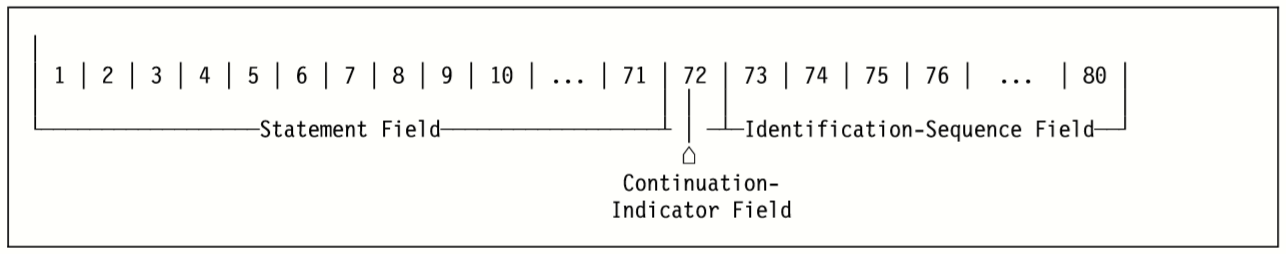
\includegraphics[width=\textwidth]{img/line}
	\caption{Description of line columns (source: \href{https://www-01.ibm.com/servers/resourcelink/svc00100.nsf/pages/zOSV2R3sc264940/$file/asmr1023.pdf}{HLASM Language Reference} ).}
	\label{fig01:line}
\end{figure}


\section{Assembling}
\label{Assembling}

Having briefly outlined the syntax, we now describe the assembly process of HLASM. 

We distinguish two types of processing:

\begin{itemize}
	\item \emph{conditional assembly (CA) processing} --- the main purpose of which is to generate statements for ordinary assembly (see \cref{CA_proc})
	\item \emph{ordinary assembly processing} --- which handles \emph{machine instructions} and \emph{assembler instructions} (see \cref{mach_instr}, \cref{asm_instrs})
\end{itemize}

\subsection{Ordinary assembly}

Ordinary assembly, along with machine and assembler instructions, is responsible for the runtime behavior of the program. It allows the generation of code from both traditional machine instructions and special-purpose assembler instructions. Moreover, it assigns values to \emph{ordinary symbols}.

\subsubsection{Ordinary symbols}
\label{ord_sym}

In HLASM, an \emph{ordinary symbol} is a named run-time constant. It is defined by inputting its name into the name field of a statement along with a special assembler instruction. Each ordinary symbol can only be defined once, and its value is constant. There are two types of ordinary symbols:
 
\begin{itemize}
	\item An \emph{absolute symbol} that simply has an integral value.
	\item A \emph{relocatable symbol} that represents an address in the resulting object code. A relocatable symbol can also be defined by writing the ordinary symbol name into the name field of a statement along with a machine instruction name. The symbol then denotes the address of the given instruction.
\end{itemize}

In addition to symbol value, ordinary symbols also contain a set of \emph{attributes}, the most common ones being \emph{type} and \emph{length}.

\subsubsection{Machine instructions}
\label{mach_instr}

\emph{Machine instructions} represent the actual processor instructions executed during run-time. Similarly to traditional assemblers, they are translated into corresponding opcodes and their operands are processed. However, HLASM also allows expressions to be passed as their operands, which may use ordinary symbols and support integer and address arithmetic.

\subsubsection{Assembler instructions}
\label{asm_instrs}

In addition to machine instructions, HLASM assembler also provides \emph{assembler instructions} (in other systems commonly termed \emph{directives}). They instruct the assembler to make specific actions rather than to assemble opcodes. For example, they generate run-time data constants, create ordinary symbols, organize the resulting object code and generally affect how the assembler operates.

Following are examples of assembler instructions:
\begin{itemize}
	\item \textbf{ICTL} --- changes values of the previously described line columns (i.e. begin column may begin at column 2 etc.).
	
	\item \textbf{DC}, \textbf{DS} --- reserves space in object code for data described in operands field and assembles them in place (i.e. assembles float, double, character array, address etc.). These instructions take \emph{data definition} as operands. \Cref{data_def_example} shows examples of data definition.
	
	\item \textbf{EQU} --- defines ordinary symbols.
	
	\item \textbf{COPY} --- copies text from a specified file\footnote{Path to the folder of the file is passed to assembler before the start of assembly} (called \emph{copy member}) and pastes it in place of the instruction. It is very similar to the C preprocessor \texttt{\#include} directive.
	
	\item \textbf{CSECT} --- creates an executable control section, which serves as the start of relative addressing. It is followed by sequence of machine instructions.
\end{itemize}

\begin{figure}[t]
	\begin{verbatim}
CL8'ABC'
    C is type of data definition - array of characters
    L8 specifies length - 8 bytes
    'ABC' is nominal value of the data definition
    CL8'ABC' would assemble 8 bytes, first three of which would be EBCDIC
             representations of letters A, B and C

5AY(A+4,B)
    5 is duplication factor - the nominal value will be repeated 5 times
    A is type - address
    Y is type extension - it modifies the length of the address
    (A+4,B) is nominal value - comma separated expressions that will
            be assembled as addresses
    5AY(A+4,B) would assemble total of 20 bytes, first 2 bytes is value
               of expression A+4, then B and then 4 more copies of the same
	\end{verbatim}
	\caption{Examples of data definition}
	\label{data_def_example}
\end{figure}

\subsubsection{Ordinary symbols resolution}
\label{ordinary_resolution}
All the assembler instructions and ordinary symbols must be resolved before the assembler creates the final object file. However, as the HLASM language supports forward declaration of ordinary symbols, the assembly may be quite complicated. Consider an example in \cref{lst:ordinary_assembly}. When the instruction on line 1 is seen for the first time, it is impossible to determine its length, because the symbol \verb|LEN| is not defined yet \footnote{Character L with an expression in parentheses in DS operand of type C specifies how many bytes should be reserved in the program.}. The same applies to the length of the instruction on the second line. Furthermore, it is also impossible to determine the exact value of relocatable symbols \verb|ADDR| and \verb|HERE| because of the unknown length of the preceding instructions.

\begin{listing}[t]
	\begin{Verbatim}[numbers=left]
           DS    CL(LEN)
ADDR       DS    CL(SIZE)

HERE       DS    0C
LEN        EQU   HERE-ADDR
SIZE       EQU   1
	\end{Verbatim}
	\caption{A sample program that shows that symbols can be used prior to their definition.}
	\label{lst:ordinary_assembly}
\end{listing}


In the next step, \verb|LEN| is defined. However, it cannot be evaluated, because the subtraction of addresses \verb|ADDR| and \verb|HERE| is dependent on the unknown length of instruction on second line and therefore on the symbol \verb|SIZE|. The whole program is resolved only when the assembly reaches the last line, which defines the length of instruction \verb|02|. Afterwards, it is possible to resolve \verb|LEN| and finally the length of instruction \verb|01|.

The dependency graph created from these principles can be arbitrarily deep and complicated, however it must not contain cycles (a symbol must not be transitively dependent on itself).

\subsection{Object file layout}

The product of ordinary assembly is an object file. Let us briefly describe its layout.

\subsubsection{Sections}

An object file consists of so-called \emph{sections}. They are user-defined (by instructions CSECT, DSECT, \ldots) and can be of different kinds, each with various properties. Absolute positions of sections within the object file are undefined --- they are determined automatically after the compilation. This also implies that all relocatable symbols are only defined relatively to the section that contains them.

\subsubsection{Location counter}
\label{loctr}

Any time a machine instruction is encountered, its opcode is outputted to the \emph{next available address}. Each section has a structure pointing to this address --- a so-called \emph{location counter}.

The user may define more location counters and then arbitrarily switch between them to state the next address for code generation. Therefore, at all times, there is one and only one location counter active, which defines where the next machine instruction will be generated.

At the end of assembly, all code denoted by location counters is assembled in a well-defined order, and so the absolute position of all relocatable symbols within their section is known.

The value of the location counter can be arbitrarily changed by the ORG instruction. It can be moved backwards or forwards (with restriction of counter underflow) to set the next address. This means that user can generate some code, move counter backwards and overwrite it. Then the ORG instruction can be used to set location counter to the next available untouched address to continue in object creation.

\subsection{Conditional assembly}
\label{CA_proc}

Conditional assembly is another feature provided by HLASM. It is essentially a macro-language built on top of a traditional assembler.

User may use conditional assembly instructions to either define \emph{variable symbols}, which can be used in any statement to alter its meaning, or to define \emph{macros} --- reusable pieces of code with parameters. Based on these instructions, conditional assembly then alters the textual representation of the source code and selects which lines will be processed next.

\subsubsection{Variable symbols}
\label{var_sym}
Variable symbols serve as compile-time variables. Statements that contain them are called \emph{model statements}.

During conditional assembly, variable symbols are substituted for their value to create a statement processable by ordinary assembly. For example, a user can write a variable symbol in the operation field and generate any instruction that can be a result of a substitution.

Variable symbols also have notion of their type --- they can be defined either as integer, boolean or string. CA instructions gather this information for different sorts of conditional branching.

\subsubsection{Sequence symbols}

A sequence symbol is important in compile-time branching. When written in a name field of a specific statement, branching instructions can use the symbol as a label to jump to the specified statement; hence, alter the further code generation.   

\subsubsection{CA instructions}
\label{ca_instr}

CA instructions are not assembled into object code. They are used to select which instructions will be processed by the assembler next.

One example of their capabilities is conditional and unconditional branching. As HLASM provides a variety of built-in binary or unary operations on variable symbols, complex conditional expressions can be created. This is important in HLASM, as the user can alter the flow of instructions that will be assembled into an executable program.

Another subset of CA instructions operates on variable symbols. These can be used to define variable symbols locally or globally, assign or update their values.

\subsubsection{Macros}

A \emph{macro} is a structure consisting of a \emph{name}, \emph{input parameters} and a \emph{body}, which is a sequence of statements. When a macro is called in a HLASM program, each statement in its body is executed. Both nested and recursive calls of macros are allowed. Macro body can also contain CA instructions, or even a sequence of instructions generating another macro definition. With the help of variable symbols, HLASM has the power to create custom, task specific macros.

\subsubsection{Description of a HLASM code example}
\label{hlasm_ex}

The current section contains description of the example shown in  \cref{lst:example}.

On lines \verb|01-04|, we see a \emph{macro definition}. It is defined with name \verb|GEN_LABEL|, variable \verb|NAME| and contains one instruction in its body, which assigns the current address to the label in \verb|NAME|.

On line \verb|06|, the \emph{copy instruction} is used, which includes the contents of the \verb|REGS| file.

Line \verb|08| establishes a start of an executable section \verb|TEST|. 

On line \verb|09|, an integer value is assigned to a variable symbol \verb|VAR|. The value is the length attribute of previously non-defined constant \verb|DOUBLE|. The assembler looks for the definition of the constant to properly evaluate the conditional assembly expression. In the next line, there is a CA branching instruction \verb|AIF|. If value of \verb|VAR| equals 4, all the text between \verb|AIF| and \verb|.END| is completely skipped and assembling continues on line \verb|18|, where the branching symbol \verb|.END| is located.

Lines \verb|12-13| show examples of machine instructions that are directly assembled into object code. Lines \verb|11| and \verb|14| contain examples of a macro call.

On line \verb|15|, the constant \verb|LEN| is assigned the difference of two addresses, which results in absolute ordinary symbol. This value is next used to generate character data.

Instruction \verb|DC| on line \verb|17| creates value of type double and assigns its address to the ordinary symbol \verb|DOUBLE|. This constant also holds information about length, type and other attributes of the data.  

\verb|ANOP| is an empty assembler action which defines the \verb|.END| symbol and line \verb|19| ends the assembling of the program. 

%\let\oldv\verbatim
%\let\oldendv\endverbatim

%\def\verbatim{\par\hspace{1cm}\setbox0\vbox\bgroup\oldv}
%\def\endverbatim{\oldendv\egroup\fboxsep0pt \colorbox[gray]{0.8}{\usebox0}\par}

\begin{listing}[t]
    \begin{verbatim}
name        operation   operands
    \end{verbatim}
	\begin{Verbatim}[numbers=left]
            MACRO                   
&NAME       GEN_LABEL
&NAME       EQU         *
            MEND
        
            COPY        REGS
        
TEST        CSECT
&VAR        SETA        L'DOUBLE
            AIF         (&VAR EQ 4).END
LBL1        GEN_LABEL
            LR          3,2
            SR          2,3
LBL2        GEN_LABEL
LEN         EQU         LBL2-LBL1
            DC          (LEN)C'HELLO'
DOUBLE      DC          H'-3.729'
.END        ANOP
            END
	\end{Verbatim} 
	\caption{An example of an artificial HLASM program (see \cref{hlasm_ex} for code description).}
	\label{lst:example}
\end{listing}

\vspace{5mm}

Although CA processing may act like text preprocessing, it is still interlinked with ordinary processing. CA has mechanics that allow the assembler to gather information about statements that are printed during the processing. It can also access values created in ordinary assembly and use them in conditional branching, and is able to lookup constants that are not yet defined prior to the currently processed statement. During ordinary assembly, names of these instructions can also be aliased.

To sum up, CA processing has variables for storing values during the compilation and CA instructions for conditional branching. Hence, it is Turing-complete while still evaluated during compile-time.

\section{HLASM source structure}

The file that generates the object code is called an \emph{open-code} file. It is the entry file of the HLASM compiler. Each open-code file can have in-file dependencies, specifically:
\begin{itemize}
	\item External Macro definitions
	\item Copy members
\end{itemize}
These are not treated as open-code files because they do not directly generate object code. Rather, they serve as statement sequences that are included in specific places of open-code and provide specific meaning.



\chapter{Architecture overview}
\label{arch}

\begin{figure}
	\centering
	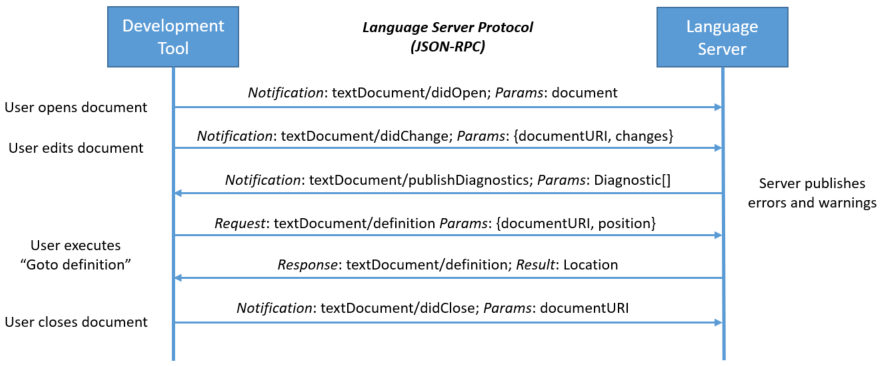
\includegraphics[width=\textwidth]{img/language-server-sequence}
	\caption[LSP session example.]{LSP session example. (source: \url{https://microsoft.github.io/language-server-protocol/overview} )}
	\label{fig04:LSP}
\end{figure}

\begin{figure}
	\centering
	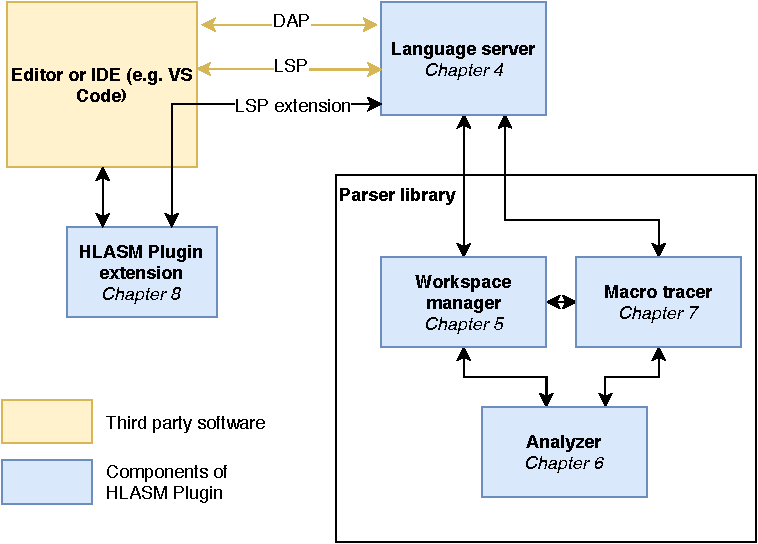
\includegraphics[width=\textwidth]{img/hlasm_architecture}
	\caption{The architecture of HLASM Plugin}
	
	\label{fig04:arch}
\end{figure}

The architecture is based on the way modern code editors and IDEs are extended to support additional languages. We chose to implement Language Server Protocol \footnote{\url{https://microsoft.github.io/language-server-protocol/}} (LSP), which is supported by a majority of contemporary editors.

In LSP, the two parties that communicate are called a \emph{client} and a \emph{language server}. A simple example is displayed in \cref{fig04:LSP} The client runs as a part of an editor. The language server may be a standalone application that is connected to the client by a pipe or TCP. All language-specific user actions (for example the Go to definition command) are transformed into standard LSP messages and are sent to the language server. The language server then analyzes the source code and sends back a response, which is then interpreted and presented to the user in editor-specific way. This architecture makes possible to only have one LSP client implementation for each code editor, which may be reused by all programming languages. And vice versa, every language server may be easily used by any editor that has an implementation of the LSP client.

To add support for HLASM, we have implemented the LSP language server and written a lightweight extension to an editor, which uses an already existing implementation of the LSP client. To implement source code highlighting, we had to extend the protocol with a new notification. This notification is used for transferring information from the language server to the VS Code client, which is extended to highlight code in editor based on the incoming custom notifications.

In this chapter, we further decompose the project into smaller components and describe their relations. The two main components are the parser library and the language server --- an executable application that uses the parser library. An overview of the architecture is pictured in \cref{fig04:arch}. The architecture of whole project is shown in \cref{all_arch}

\section{Language server component}

The responsibility of the language server component is to maintain the LSP session, convert incoming JSON messages and use the parser library to execute them. The functionality includes:
\begin{itemize}
    \item reading LSP messages from either a standard input or TCP and writing responses
    \item parsing JSON RPC to C++ structures, so they can be further used
    \item serializing C++ structures into JSON, so it can be sent back to the client
    \item asynchronous request handling: when a user makes several consecutive changes to a source code, parsing on every change is not needed
\end{itemize}

\section{Parser library component}

Parser library is the core of the project --- it encapsulates the analyzer, which provides all parsing capabilities, and workspace manager, which keeps track of open files in the editor and manages their dependencies. It has to keep the representation of workspaces and files in the parser library exactly the same as the user sees in the editor. It also starts the analyzer when needed, manages workspace configuration and provides external macro and copy libraries to analyzer.

\subsection{Parser library API}
The parser library API is based on LSP --- every relevant request and notification has a corresponding method in the parsing library.

At first, the API implements the LSP notifications that ensure the editor state synchronization. Apart from working with individual files, the LSP also supports workspaces. A workspace is basically just a folder that contains related source codes. The LSP also supports working with multiple workspaces at the same time. We use it when searching for dependencies of HLASM source codes (macros, and copy files).

The parser library has the exact contents of all files in open workspaces. To achieve that, there is a file watcher running in the LSP client that notifies the server when any of the HLASM source files is changed outside of editor. For example, when a user deletes an external macro file, the parser library should react by reporting that it cannot find the macro.

The list of necessary editor state synchronization notifications follows:
\begin{itemize}
	\item Text synchronization notifications (\TT{didOpen}, \TT{didChange}, \TT{didClose}) that inform the library about files that are currently open in the editor and their exact contents.
	\item \TT{DidChangeWorkspaceFolders} notification that informs the library when a workspace has been opened or closed.
	\item \TT{DidChangeWatchedFiles} notification
\end{itemize}

Next, the API implements the requests and notifications that provide the parsing results, specifically:
\begin{itemize}
	\item \TT{publishDiagnostics} notification. A diagnostic is used to indicate a problem with source files, such as a compiler error or a warning. The parser library provides a callback to let the language server know that diagnostics have changed.
	\item Callback for highlighting information provision.
	\item Language feature requests (\TT{definition}, \TT{references}, \TT{hover}, \TT{completion}), which provide information needed for proper reaction of the editor on user actions.
\end{itemize}

\subsection{Analyzer}

The analyzer processes a single HLASM file. It takes the contents of a source file by common string and a callback that can parse external files with specified name. It provides a list of diagnostics linked to the file, highlighting, list of symbol definitions, etc.

The analysis of HLASM code includes:
\begin{itemize}
 \item recognition of statements and their parts (lexing and parsing)
 \item interpretation of instructions that should be executed in compile time
 \item reporting of problems with the source by producing LSP diagnostics
 \item providing highlighting and LSP information
\end{itemize}

A HLASM source files have dependencies --- other files that define macros or files brought in by the COPY instruction. Dependencies are only discovered during the processing of files, so it is not possible to provide the files with macro definitions beforehand. The analyzer gets a callback that finds a file with specified name, parse its contents and return it as a list of parsed statements. 

\section{Client-side VS Code extension}
\label{arch:client}

The VS Code extension component ensures seamless integration with the editor. Its functions are:

\begin{itemize}
	\item to start the HLASM language server and the LSP client that comes with VS Code, and to create a connection between them.
	\item to implement extension of the LSP protocol for enabling server-side highlighting. The extended client parses the information from the server and uses VS Code API to actually color the text in the editor.
	\item to implement support for editing lines with continuations --- when the user types something in front of the continuation character, it should stay in place.
\end{itemize}


\section{Macro tracer}
\label{arch:macro}
The macro tracer gives a possibility to trace the compilation of HLASM source code in a way similar to common debugging. This is the reason why we chose to implement support for the Debug Adapter Protocol \footnote{\url{https://microsoft.github.io/debug-adapter-protocol/}} (DAP). It is very similar to LSP, so most of the code implementing LSP in the language server component may be reused for both protocols.

The language server component communicates with the macro tracer component in the parser library. Its API mirrors the requests and events of DAP.

The main responsibilities of the macro tracer include:

\begin{itemize}
	\item \TT{launch}, \TT{continue}, \TT{next}, \TT{stepIn} and \TT{disconnect} requests, which allow the user to control the flow of the compilation
	\item \TT{SetBreakpoints}, which transfers the information about breakpoints that the user has placed in the code
	\item \TT{Threads}, \TT{StackTrace}, \TT{Scopes} and \TT{Variables} requests to allow the DAP client to retrieve information about the current processing stack (stack of nested macros and copy instructions), available variable symbols and their values
	\item \TT{stopped}, \TT{exited} and \TT{terminated} events to let the DAP client know about state of traced source code
\end{itemize}

The macro tracer communicates with the workspace manager to retrieve the content of the traced files. It analyzes the source file in a separate thread and gets callbacks from the analyzer before each statement is processed. In the callback, the tracer puts the thread to sleep and waits for user interaction. During this time, it is possible to retrieve all variable and stack information from the processing to display it to the user.


\part{Component description}
\chapter{Language server}
\index{language\_server@\texttt{language\_server}}
\label{chap:lang_server}
The purpose of the Language server is to implement the Language Server Protocol (LSP) and the Debug Adapter Protocol (DAP) and to provide access to the parser library by using them. It has to deserialize and serialize LSP and DAP messages, extract parameters of particular methods and then serve the requests by invoking functionality of parser library.

\section{Language Server Protocol}
Language Server Protocol is used to extend code editors with support for additional programming languages. LSP defines 2 communicating entities: a client and a server. The LSP client is editor-specific and wraps interaction with the user. The LSP server is language-specific and provides information about the source code.

The main purpose of the LSP is to allow the language server to provide language-specific response to various user interactions with the code editor. Messages that flow through LSP can be divided into three categories:

\begin{itemize}
	\item \textbf{Parsing results presentation} Messages from the first category allow the language server to send results of source code analysis to the LSP client. The editor is then able to show them to the user. For example, when the user clicks on a symbol in HLASM code and then uses the `Go to definition' function, the LSP client sends a request to the language server with the name of currently open file and current location in the file. The server is then expected to send back the location of the definition, so the editor can present it to the user (e.g. the editor moves the caret to the definition location). List of all such messages is in \cref{lsp_parse_results}.

	\item \textbf{Editor state and file content synchronization} Messages from the second category flow mainly from the client to the server and ensure that the server has enough information to correctly analyze source code. List of all such messages can be found in \cref{lsp_text_sync_methods}.
	
	\item \textbf{LSP initialization and finalization} Lastly, there are several messages that handle protocol initialization and finalization.
\end{itemize}


\begin{table}
	\centering
	\begin{tabular}{ll}
		
		\toprule
		Message & Description \\ \midrule
		& \multirow{3}{9cm}{The client sends a position in an open file. The server responds with a position of a definition of a symbol at that position.} \\
		textDocument/definition &  \\
		& \\
		& \\
		& \multirow{3}{9cm}{The client sends a position in an open file. If there is a symbol, the server responds with a list of positions where the symbol is used.}\\
		textDocument/references & \\
		& \\
		& \\
		& \multirow{3}{9cm}{The client sends a position in an open file where the user is pointing with the cursor. The server responds with a string to be shown in a tooltip window.}\\
		textDocument/hover & \\
		& \\
		& \\
		& \multirow{3}{9cm}{The client sends a position in an open file and how a completion box was triggered (i.e. with what key, automatically/manually). The server responds with a list of strings suggested for completion at the position.}\\
		textDocument/completion & \\
		& \\
		& \\
		& \\
		\multirow{3}{4cm}{textDocument/\\publishDiagnostics} & \multirow{3}{9cm}{The server sends diagnostics to the client. A diagnostic represents a problem with the source code, e.g. compilation errors and warnings.}\\
		 & \\
		& \\ \bottomrule
	\end{tabular}
	
	\caption{List of all results-presenting messages}
	\label{lsp_parse_results}
\end{table}

\begin{table}
	\centering
	\begin{tabular}{ll}
		
		\toprule
		Message & Description \\ \midrule
		textDocument/didOpen & \multirow{3}{8.5cm}{The server is notified whenever the user opens a file, changes contents of an already open file or closes a file in the editor.} \\
		textDocument/didChange & \\
		textDocument/didClose & \\
		& \\
		 &\multirow{4}{8.5cm}{The client notifies the server when a watched file is changed outside of the editor. Watched files selector is defined when the client is started (in the extension component).} \\
		workspace/ & \\
		didChangeWatchedFiles& \\
		& \\
		& \\
		workspace/ & \multirow{2}{8.5cm}{The client notifies the server that the user has opened or closed a workspace.} \\
		didChangeWorkspaceFolders & \\ \bottomrule
	\end{tabular}
	
	\caption{List of all implemented editor state and text synchronization messages}
	\label{lsp_text_sync_methods}
\end{table}


LSP is based on JSON RPC\footnote{\url{https://www.jsonrpc.org/specification}}. There are two types of interaction in JSON RPC: requests and notifications. Both of them carry the information to invoke a method on the recipient side ---  name of the method and its arguments. The difference between the two is that each request requires a response containing the result of the method, whereas the notifications do not.

The LSP uses the JSON RPC specification and further specifies how messages are transferred and defines methods, their arguments, responses and semantics. A raw message sent from the client to the server is shown in \cref{hover_message}.

\begin{listing}
	\begin{verbatim}
Content-Length: 123\r\n
\r\n
{"jsonrpc":"2.0","method":"textDocument/didClose","params":{"textDocument":
{"uri":"file:/c%3A/Users/admin/Documents/source.hlasm"}}}
	\end{verbatim}
	\caption{An example of a message sent from the client to the server.}
	\label{hover_message}
\end{listing}

The raw messages have HTTP-like headers. The only mandatory header is \TT{Content-Length}, which tells the recipient the length of the following message. The JSON itself is sent after the header.

Inside the JSON, there is a name of the method to be invoked and parameters to pass to the method. In this case, the client is sending a notification that file \TT{C:/Users/admin/Documents/source.hlasm} was closed in the editor by the user. As it is a notification, there must not be any response.

On top of this basic protocol, LSP defines methods and their semantics to cover common functionality that users expect when programming in an editor. List of all methods implemented in the language server can be found in \cref{LSP_methods}.

\section{DAP}
Debug Adapter Protocol is used to extend code editors with debugging support for additional programming languages. We use it to provide the user with the ability to trace how the HLASM compiler processes source code step by step. The user can see the values of compile-time variables and follow the expansion of macros in debug-like experience.

The communication in DAP is between an editor or an IDE and a debugger. The editor notifies the debugger about the user actions, e.g. when a breakpoint is set or when the user uses step in/step over buttons. The debugger informs the editor about the state of the debugged application, for example when the debugger stopped because it hit a breakpoint. While it is stopped, the debugger sends information about program stack, variables valid in current debugger scope and its values.

DAP is very similar to LSP. Although the ideas behind DAP are nearly the same, DAP is not based on the JSON RPC. Instead, DAP specifies its own implementation of remote procedure call, still using JSON as the basic carrier of the messages. DAP has requests and events --- requests always go from the client to the server and require response. Events are the same as the notifications from JSON RPC that are sent from the server to the client. The similarity allows our language server component to share a lot of code between the implementations of the protocols.

\section{Language server overview}
The architecture of the Language server component is illustrated in \cref{lang_server_arch}. It communicates on the standard input/output via LSP with the LSP client and listens on a TCP port to provide DAP support for the macro tracer. The TCP communication is wrapped by class \TT{tcp\_handler}, which abstracts from the complexity of communicating through TCP/IP.


\begin{figure}
	\centering
	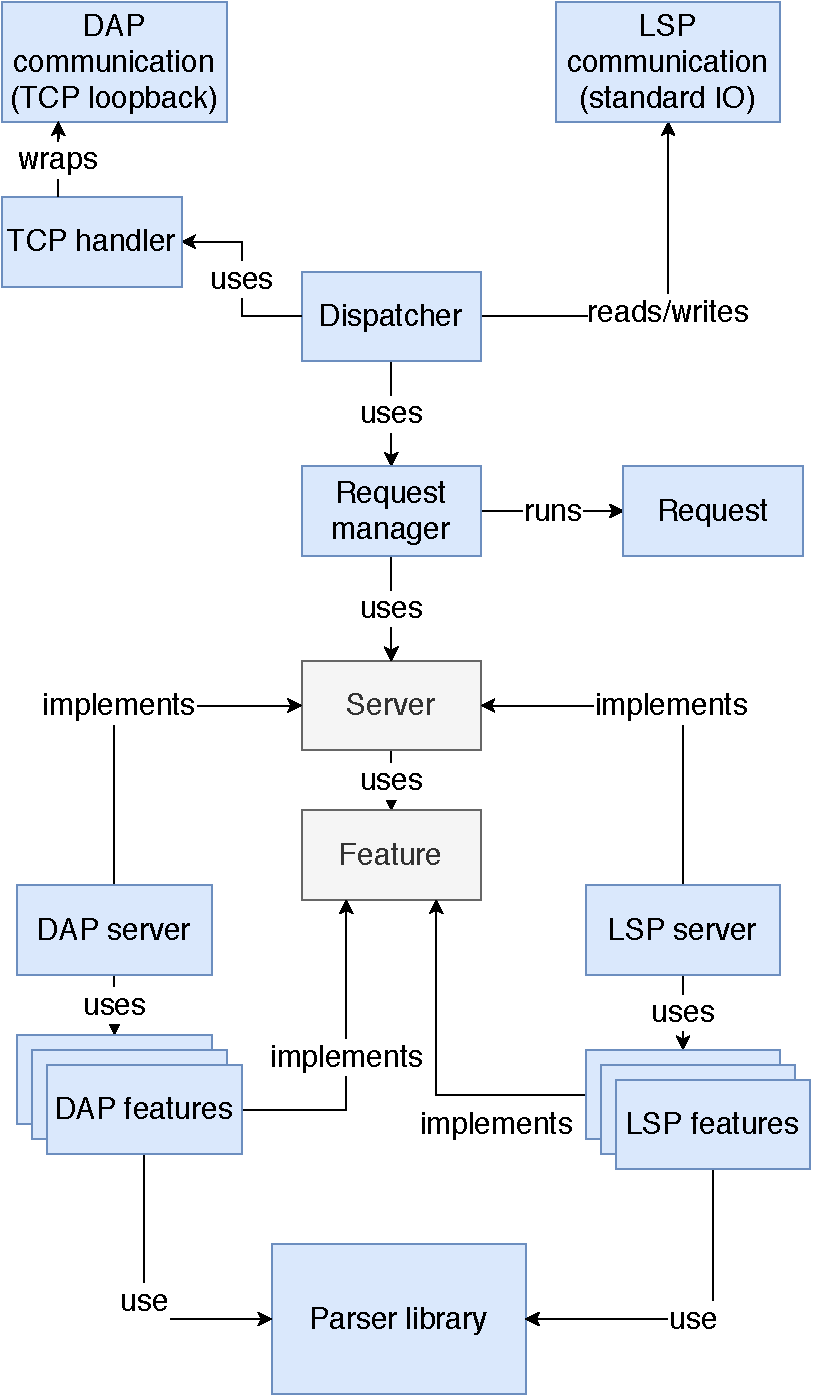
\includegraphics[width=11cm]{img/lang_server}
	\caption{Architecture of language server.}
	\label{lang_server_arch}
\end{figure}


The main purpose of the class \TT{dispatcher} is to provide abstraction for the lowest level communication, which is shared by LSP and DAP. It reads iostream to parse messages using the JSON for Modern C++ library (see \cref{3rd_party}) and stores them in the \TT{request\_manager} as \TT{requests}.

A \TT{request} encapsulates one message that came from the client and is basically represented only by raw (but parsed) JSON.

\TT{request\_manager} stores \TT{requests} in a queue and runs a worker thread that serves the requests one by one. As there is only one instance of \TT{request\_manager} running in the language server, it serializes requests from DAP and LSP (which come asynchronously from separate sources) into one queue.

\TT{server} is an abstract class that implements protocol behavior that is common for both DAP and LSP --- it basically implements Remote Procedure Call. Actual handling of LSP and DAP requests is implemented in \TT{features}. Each \TT{feature} contains implementation of several protocol requests or notifications. The features unwrap the arguments from JSON and call corresponding parser library methods.

There are two implementations of the abstract \TT{server} class: \TT{lsp\_server} and \TT{dap\_server}. They both implement the initialization and finalization of protocol communication, which is a bit different for both protocols and both use features to serve protocol requests.

\section{Example: hover request handling}

\afterpage{
	\begin{landscape}
		\begin{figure}
			\centering
			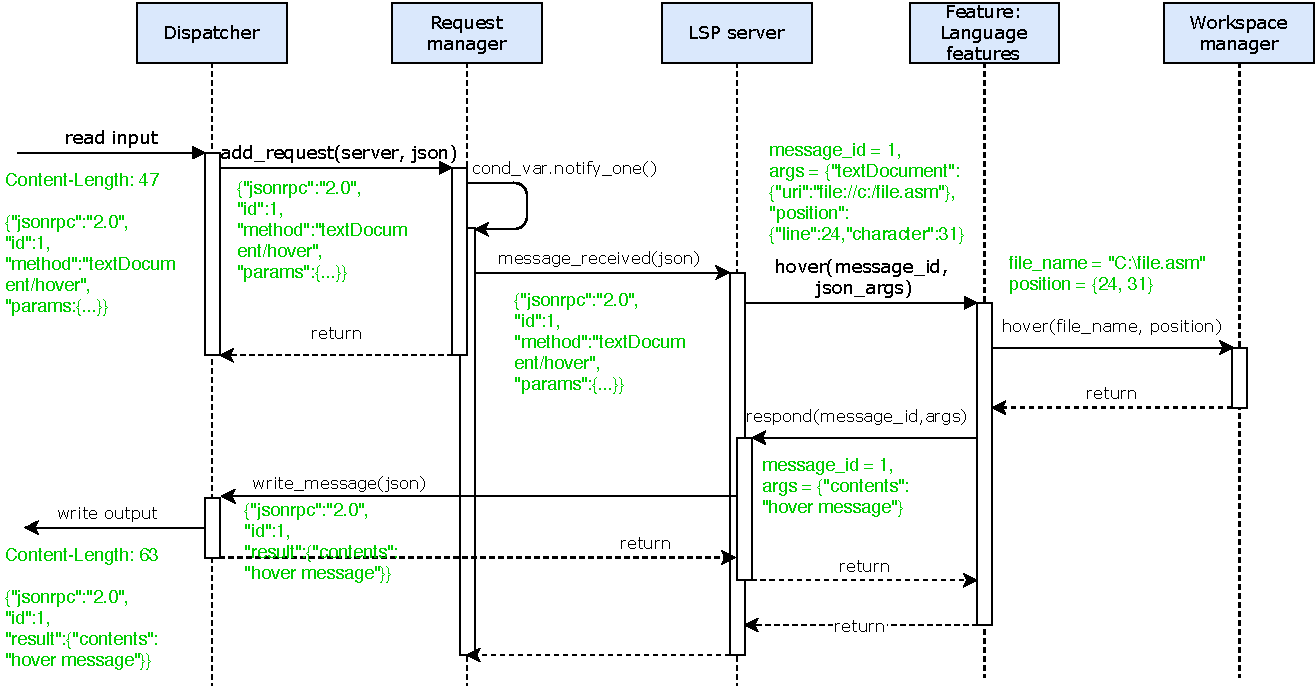
\includegraphics[width=21cm]{img/hover_sequence}
			\caption{A sequence diagram showing the processing of the textDocument/hover request in the language server. The green text represents an example of data passed in the arguments.}
			\label{hover_sequence}
		\end{figure}
	\end{landscape}
}

The \cref{hover_sequence} shows handling of the hover request in the language server. The hover request is sent from the LSP client to the \TT{lsp\_server} when the user hovers over the text of a file. The hover request contains location of the mouse cursor in text, i.e. the name of the file, the number of line and column where the cursor is. The LSP client then expects a response containing a string (possibly written in markdown language) to be shown in a tooltip box.

The whole process begins with reading from the standard input by the LSP instance of the \TT{dispatcher}. It first reads the header of the message, which contains the information about the length of the following JSON. Then it reads the JSON itself and deserializes it using the JSON for Modern C++ library (see \cref{3rd_party}). All other components of the language server work only with the parsed representation of the message. The \TT{dispatcher} adds the message to the \TT{request\_manager} and returns to reading the next message from the standard input.

The request in the \TT{request\_manager} either waits in a queue to be processed, or, if the queue was empty, the worker thread is woken up from sleep using conditional variable. The worker then passes the JSON to the \TT{lsp\_server}, which looks at the name of the method written in the message and calls the method ``hover'' from the language feature.

The hover method unpacks the actual arguments from JSON and converts any URIs to paths using the cpp-netlib URI library. Then, it calls the hover method from the parser library, which returns a string to be shown in the tooltip next to the hovering mouse. The language feature then wraps the return value back in JSON and calls the \TT{respond} method of its \TT{response\_provider} implemented by the \TT{lsp\_server}.

The \TT{lsp\_server} wraps JSON arguments into a LSP response and uses the \TT{send message provider} implemented by \TT{dispatcher} to send it to the LSP client. The \TT{dispatcher} serializes the JSON, adds the header with the length of the JSON and writes the message to a standard output. Finally, all methods return and the worker thread in \TT{request\_manager} looks for another request. If there is none, it goes to sleep.

%******************** IO HANDLING *************************
\sectionSrc{I/O handling}
{language\_server/src/main.cpp,language\_server/src/dispatcher.h,language\_server/src/dap/tcp\_handler.h}

The purpose of the \TT{dispatcher} is to abstract from the complexity of working with raw strings and streams. It executes an infinite loop in which it reads messages from \TT{std::iostream} and adds them to the \TT{request\_manager} as parsed JSON objects. At the same time, it is able to write responses in the correct format.

The language server communicates with the LSP client on a standard input and output, so we simply use the \TT{dispatcher} with the standard \TT{std::cin} and \TT{std::cout} objects to communicate with the LSP client.

The DAP communicates using TCP/IP, which is less straightforward. Before the VS Code extension starts the language server, it finds a free TCP port and passes it as an argument to the language server executable. The \TT{TCP handler} then starts listening on that port. Once the user wants to start the macro tracer, the DAP client connects to the port on localhost. The \TT{tcp\_handler} accepts the TCP client and creates a \TT{dispatcher} and a \TT{dap\_server}. Once the DAP communication ends, both the \TT{dispatcher} and the \TT{dap\_server} are destroyed and the \TT{tcp\_handler} starts listening again for the next DAP session. Thanks to the ASIO library (see \cref{3rd_party}) implementation of the \TT{std::iostream} interface, the \TT{dispatcher} is able to completely abstract from the fact that it is communicating through TCP and not through the standard IO.

%******************** SERVERS *************************
\sectionSrc{LSP and DAP Server}
{language\_server/src/server.h,language\_server/src/feature.h,language\_server/src/lsp/lsp\_server.h,language\_server/src/dap/dap\_server.h,language\_server/src/dap/dap\_feature.h}
The servers are able to process incoming LSP and DAP requests. They get the messages in a form of already parsed JSONs. Then they extract the name of the requested method with its parameters from the message and call the corresponding method with the parameters encoded as JSON.

There are two server implementations: \TT{lsp\_server} and \TT{dap\_server}. Both inherit from an abstract class called \TT{server}. They implement protocol-specific processing of messages --- although the protocols are quite similar (both are based on RPC), each protocol has different initialization and finalization, different message format, etc.

The functionality of servers is divided into \TT{features}. Each feature implements several LSP or DAP methods by unpacking the arguments of the respective method and calling corresponding parser library function. During initialization, each feature adds its methods to the server's list of implemented methods. The \TT{lsp\_server} uses three features:
\begin{itemize}
	\item \emph{Text synchronization feature}, which handles the notifications about the state of open files in the editor.
	\item \emph{Workspace folders feature}, which handles the notifications about adding and removing workspaces.
	\item \emph{Language feature}, which handles requests about HLASM code information.
\end{itemize}
The \cref{LSP_methods} shows the list of all implemented LSP methods and the classes where the implementations lie.

\begin{table}
	\centering
	\begin{tabular}{lll}
		\toprule
		             \textbf{Component}   &       \textbf{LSP Method name}                                                                                          \\ \midrule
		\multirow{4}{7cm}{LSP server  \\ \srcstyle{language\_server/src/lsp/lsp\_server.h}}                                  & initialize                           \\
		                                                                                                                     & shutdown                             \\
		                                                                                                                     & exit                                 \\
		                                                                                                                     & textDocument/publishDiagnostics      \\ \midrule
		\multirow{4}{7cm}{Text synchronization feature \srcstyle{language\_server/src/lsp/feature\_text\_synchronization.h}} & textDocument/didOpen                 \\
		                                                                                                                     & textDocument/didChange               \\
		                                                                                                                     & textDocument/didClose                \\
		                                                                                                                     & textDocument/semanticHighlighting    \\ \midrule
		\multirow{2}{7cm}{Workspace folders feature \srcstyle{language\_server/src/lsp/feature\_workspace\_folders.h}}       & workspace/didChangeWorkspaceFolders  \\
		                                                                                                                     & workspace/didChangeWatchedFiles      \\ \midrule
		\multirow{4}{7cm}{Language feature \srcstyle{language\_server/src/lsp/feature\_language\_features.h}}                & textDocument/definition              \\
		                                                                                                                     & textDocument/references              \\
		                                                                                                                     & textDocument/hover                   \\
		                                                                                                                     & textDocument/completion              \\ \bottomrule& 
	\end{tabular}
	\caption{The list of all implemented LSP methods and the classes where they are implemented}
	\label{LSP_methods}
\end{table}

The DAP server uses only one feature --- the Launch feature, which handles stepping through the code and retrieving information about both variables and stack trace. The table \cref{DAP_methods} shows the list of all implemented DAP methods.

\begin{table}
	\centering
	\begin{tabular}{lll}
		\toprule
		\textbf{Class}                          & \textbf{Source file}                                                      & \textbf{DAP Method name} \\ \midrule
		\multirow{2}{3cm}{\TT{dap\_server}}      & \multirow{2}{3cm}{\srcstyle{language\_server/src/dap/dap\_server.h}}      & \TT{initialize}          \\
		                                        &                                                                           & \TT{disconnect}          \\ \midrule
		\multirow{13}{3cm}{\TT{launch\_feature}} & \multirow{13}{3cm}{\srcstyle{language\_server/src/dap/feature\_launch.h}} & \TT{launch}              \\
		                                        &                                                                           & \TT{setBreakpoints}      \\
		                                        &                                                                           & \TT{configurationDone}   \\
		                                        &                                                                           & \TT{threads}             \\
		                                        &                                                                           & \TT{stackTrace}          \\
		                                        &                                                                           & \TT{scopes}              \\
		                                        &                                                                           & \TT{next}                \\
		                                        &                                                                           & \TT{stepIn}              \\
		                                        &                                                                           & \TT{variables}           \\
		                                        &                                                                           & \TT{continue}            \\
		                                        &                                                                           & \TT{stopped}             \\
		                                        &                                                                           & \TT{exited}              \\
		                                        &                                                                           & \TT{terminated}          \\ \bottomrule
	\end{tabular}
	\caption{The list of all implemented DAP methods and the classes where they are implemented}
	\label{DAP_methods}
\end{table}

%******************** RESPONSE *************************
\sectionSrc{Response with result}
{language\_server/src/feature.h,language\_server/src/server.h}

According to the LSP and the DAP, the server is required to send messages back to the LSP/DAP client either as responses to requests (e.g. \TT{hover}), notifications (e.g. textDocument/publishDiagnostics notification) or events (e.g. stopped event). Features require reference to an instance of the \TT{response\_provider} interface that provides methods \TT{respond} and \TT{notify} for sending messages back to the LSP client. Both LSP and DAP server classes implement the \TT{response\_provider} to form protocol-specific JSON with the arguments.

The servers then send the JSON to the LSP/DAP client using the \TT{send\_message\_provider} interface. At this point, the final complete JSON response is formed. The \TT{send\_message\_provider} then adds the message header and serializes the JSON using the JSON for Modern C++ library (see \cref{3rd_party}).

The only implementation of the \TT{send\_message\_provider} interface is the \TT{dispatcher}.

%******************** REQUEST MANAGER *************************
\sectionSrc{Request Manager}
{language\_server/src/request\_manager.h}

\TT{request\_manager} encapsulates a queue of requests with a worker thread that processes them. There may be up to two \TT{dispatcher} instances in the language server: one for LSP and one for DAP. Both of them add the requests they parse into one \TT{request\_manager}. It is necessary to process the requests one by one, because the parser library cannot process more requests at the same time.

Asynchronous communication is handled by separating the communication into threads:
\begin{itemize}
	\item LSP read thread --- a thread in which the \TT{dispatcher} reads messages from the standard input.
	\item DAP read thread --- a thread in which the \TT{tcp\_handler} listens on a localhost port to initiate a DAP session. After accepting the DAP client, the \TT{dispatcher} reads DAP input on this thread too.
	\item Worker thread in \TT{request\_manager} that processes each request using the \TT{lsp\_server} or the \TT{dap\_server} and ultimately the parser library.
\end{itemize}

The threads are synchronized in two ways: First, there is a mutex that prevents the LSP and the DAP threads from adding to the request queue simultaneously. Second, there is a conditional variable to control the worker thread.

\TT{request\_manager} additionally incorporates a mechanism for invalidating requests that have been obsoleted by new requests. The obsoleting of requests is done by a cancellation token. It is shared between the parser library and the \TT{request\_manager}. When set to true, the results of current request or notification are no longer needed, the parser library stops all parsing and return as soon as possible.

When a new request arrives, all previous requests (including the currently processed one) that concern the same file are invalidated. However, they cannot be simply removed from the queue. They still have to be processed as they may carry information that must not be discarded (e.g. changes to contents of a file). The parser library processes the request but does not reparse any source files.

\subsection{Example of request invalidating}

For example, when a user starts changing a file, every character he writes is passed to the language server as a textDocument/didChange notification. Each such notification is processed in two stages:
\begin{enumerate}
	\item The parser library changes the internal representation of the text document.
	\item The parser library starts the parsing of the file to update diagnostics and highlighting. This may take some time.
\end{enumerate}
When more didChange notifications come in succession, their first parts must be executed with all the notifications to keep the internal representation of the file updated. However, the user is interested only in diagnostics and semantic highlighting for the current state of the text, so we need to parse the file only once --- after the last notification.




\chapter{Workspace Manager}
\label{ws_manager}
Workspace manager encapsulates all functionality of the parser library. It is the access point to all parsing capabilities, keeps the current state of all open files and resolves libraries needed by the analyzer. It also manages when files should be reparsed.


%******************** Parser library API *************************
\sectionSrc{Parser library API}
{parser\_library/include/protocol.h,parser\_library/include/range.h,parser\_library/include/workspace\_manager.h,parser\_library/src/workspace\_manager\_impl.h}
First of all, the workspace manager component is the only public interface of the parser library. The API design is based on LSP and DAP, most of the API is just LSP/DAP rewritten in C++. The API uses the observer pattern for DAP events and notifications originating in parser library (e.g. textDocument/publishDiagnostics).

The API methods can be divided into three categories:
\begin{itemize}
	\item Editor state and file content synchronization (\cref{text_sync_methods})
	\item Parsing results presentation 
	\item Macro tracer
\end{itemize}

\subsection{Editor state and file content synchronization}

\begin{table}
	\centering
	\begin{tabular}{ll}
		
		\toprule
		Method & Description \\ \midrule
		\TT{did\_open (file name, file content)} & \multirow{3}{8cm}{Three methods that are called whenever the user opens a file, changes contents of an already opened file or closes a file in the editor.} \\
		\TT{did\_change (file name, changes)}& \\
		\TT{did\_close (file name)}& \\
		& \\
		\multirow{3}{5cm}{\TT{did\_change\_watched\_files (file paths)}} &\multirow{3}{8cm}{Method, that is called when a file from a workspace has been changed outsize of the editor} \\
		& \\
		& \\
		& \\
		\TT{add\_workspace (ws name, ws path)} & \multirow{2}{8cm}{Methods that are called when the user opens or closes a workspace in the editor} \\
		\TT{remove\_workspace (ws path)} & \\ \bottomrule
	\end{tabular}
	
	\caption{List of all Editor state and text synchronization methods}
	\label{text_sync_methods}
\end{table}

All the methods from the first category are listed in \cref{text_sync_methods}. There are two types of files that need to be synchronised:
\begin{itemize}
	\item Files, that the user has opened in the editor. Those files are being edited by the user and their content may be different from the files actually saved in the filesystem.
	\item Files, that the parser library opens from the hard disk, because they are needed to parse opened files (e.g. a macro that is used by an opened file)
\end{itemize}

So the parser library is allowed to load arbitrary files from the disk, and use its contents until such file is opened in the editor. From that point on, the only source of truth for the contents of the file are the did\_change notifications. Once the file is closed in the editor, the parser library is again allowed to rely on its contents in the filesystem.



\subsection{Parsing results presentation}

\begin{table}
	\centering
	\begin{tabular}{ll}
		
		\toprule
		Method & Description \\ \midrule
		& \multirow{3}{8cm}{The method gets a position in an opened file. If there is a symbol, the method returns position of definition of that symbol} \\
		\TT{definition(file name, caret position)} &  \\
		& \\
		& \\
		& \multirow{3}{8cm}{The method gets a position in an opened file. If there is a symbol, the method returns list of positions where the symbol is used}\\
		\TT{references(file name, caret position)} & \\
		& \\
		& \\
		& \multirow{3}{8cm}{The method gets a position in an opened file where the user points with cursor. Returns list of strings to be shown in a tooltip window}\\
		\TT{hover(file name, mouse position)}& \\
		& \\
		& \\
		& \multirow{3}{8cm}{The method gets a position in an opened file and how the completion box was triggered (i. e. with what key, automatically/manually). Returns list of strings suggested for completion at the position}\\
		\TT{completion(file name,}& \\
		\TT{mouse position, trigger info)}& \\
		& \\
		& \\ \bottomrule
	\end{tabular}
	
	\caption{List of all parse results methods}
	\label{parse_results}
\end{table}

All the methods from the second category are listed in \cref{parse_results}. They get position of caret or mouse cursor in a file and are expected to return information about the place in the code. For example, method \TT{hover} is called when the user points at some word in the code and waits for a short time. The method returns a string that the editor shows in the tooltip window at the position. Typically, the tooltip would show type of the variable and its value, if known.

Additionally, the parser library presents its results using the observer pattern. There are two interfaces: highligting and diagnostics consumer. Each of them has method \TT{consume} that gets updated information as parameter whenever there is an update. Any potential user of the library (e.g. the language server component) just has to implement the interfaces to process the results.

\subsection{Macro tracer}

The macro tracer part of the API is again just DAP rewritten in C++. There are methods that are called when the user clicks on buttons to control the macro tracer: launch the tracer, step in, step over, continue and stop. Moreover, there are methods that retrieve information about current state of traced code: stack of macro calls and information about compile time variables. See \cref{macro_tracer} for full description of macro tracer.

\section{Libraries configuration}
\label{libs_config}
The parser library approaches the dependency resolution in a way similar to the mainframe. On mainframe, you would have to define the locations of your dependencies in a JCL file \footnote{\url{https://www.ibm.com/support/knowledgecenter/zosbasics/com.ibm.zos.zjcl/zjclc_basicjclconcepts.htm}}. As the user may want to include tens of dependencies for multiple open codes, a source code management tool called Endevor\footnote{\url{https://en.wikipedia.org/wiki/Endevor}} groups these dependencies into so-called \emph{processor groups}. Then, the user only has to assign a processor group to the open code and the Endevor does the dependency resolution for him.

To provide similar experience with local files, the parser library simulates this behavior. If the user wants to include dependencies in his project, he has to define 2 configuration files inside his workspace: \emph{pgm\_conf.json} and \emph{proc\_grps.json}. The workspace component of the parser library then processes the configurations, retrieving their values upon initialization. Moreover, each time a save command is issued on any configuration file, the configuration values are reloaded via \TT{load\_config} method.

\subsection{Processor groups}

The proc\_grps configuration file contains a JSON array of possible processor groups, which consist of a name and an array of folder paths (may be relative to the root of the workspace). An example can be found in \cref{lst:proc_grps}.

Whenever \TT{load\_config} is called, the workspace retrieves these processor groups from the configuration file and creates libraries. The libraries provide information about paths to their dependency files. During the parsing, the workspace retrieves the library corresponding to the provided processor group name and uses it to search for a wanted macro or copy file. 

\subsection{Program configuration}

The pgm\_conf configuration file contains a JSON array of program names (or wildcards~\ref{section:wildcard}), matched to their processor groups. It serves as a list of the HLASM open code files and states the libraries (in form of processor groups) that contain the dependencies of each open code. An example can be found in \cref{lst:pgm_conf}.


From this configuration, the workspace simply remembers the processor group - open code mapping.


\begin{listing}[t]
	\begin{verbatim}
	{
	  "pgroups": [
	    {
	      "name":"GROUP1",
	      "libs": [
	        "ASMMAC/",
	        "C:/SYS.ASMMAC"
	      ]
	    },
	    {
	      "name":"GROUP2",
	      "libs": [
	        "G2MAC/",
	        "C:/SYS.ASMMAC"
	      ]
	    }
	  ]
	}
	\end{verbatim}
	\caption{A processor group configuration file}
	\label{lst:proc_grps}
\end{listing}

\begin{listing}[t]
	\begin{verbatim}
	{
	  "pgms": [
	    {
	      "program": "source_code",
	      "pgroup": "GROUP1"
	    },
	    {
	      "program": "second_file",
	      "pgroup": "GROUP2"
	    },
	  ]
	}
	\end{verbatim}
	\caption{A program configuration file}
	\label{lst:pgm_conf}
\end{listing}

\section{Architecture overview}
The architecture of the parser library is organized into the following components:

\begin{description}
	\item[Workspace manager API] The workspace manager provides API for handling various workspace management (e.g. add new workspace), LSP and DAP requests. It may hold multiple workspaces and calls 
	file manager to handle changes in the workspace files.
	\item[Workspace representation] The representation of workspace deals with the relations between its files (dependencies) upon parse request and propagates the parsing further into analyzer. It also retrieves data from the configuration files and it is used for resolving dependency searches by implementing parse library provider.
	\item[Processor group representation] \sectionFiles{.45\linewidth}{parser\_library/src/workspaces/processor\_group.h} 
	The representation of a processor group uses the API of libraries to search for their dependencies. Currently, we only support local libraries, which utilize the file manager for their file information retrieval.
	\item[File manager] \sectionFiles{.45\linewidth}{parser\_library/src/workspaces/file\_manager.h}
	The file manager is used by multiple components to handle file management and file searches. It also distinguishes and does conversions between regular files and processor files, which may be used for parsing.
	\item[Analyzer] The analyzer accepts a file along with the information needed for dependency resolution, syntactically and semantically processes it and fills the context tables. The component is further explained in~\cref{chap:analyzer}.
\end{description}

An overview of the architecture is visualised in~\cref{ws_mngr_arch}.

The technical details of each component are further explained in the following sections.

\afterpage{
\begin{landscape}
\begin{figure}
	\centering
	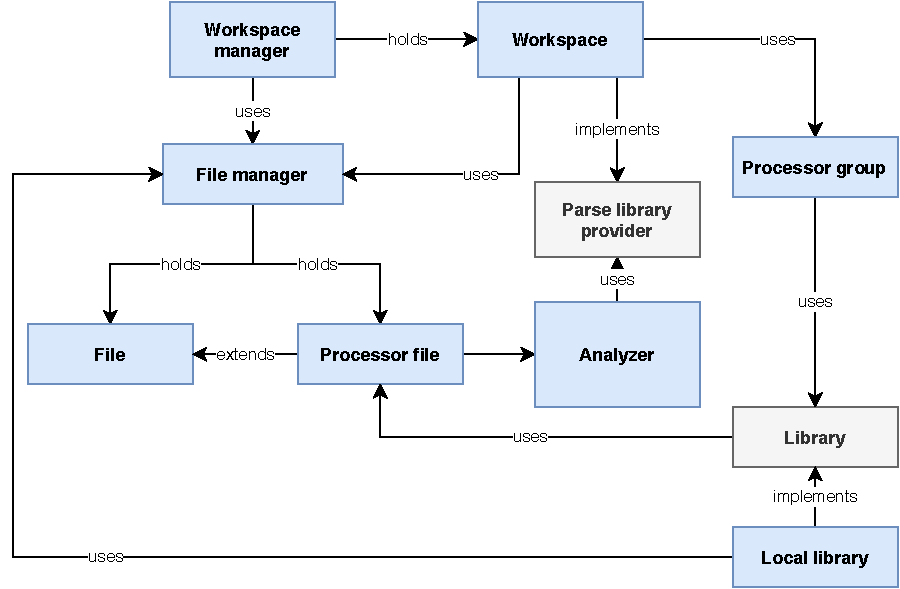
\includegraphics[width=16cm]{img/ws_mngr_arch}
	\caption{Architecture of workspace manager.}
	\label{ws_mngr_arch}
\end{figure}
\end{landscape}
}

%******************** Workspace *************************
\sectionSrc{Workspace representation}
{parser\_library/src/workspaces/workspace.h}

In VSCode, as in many other editors, a grouping of files for a single project is called the \emph{workspace}. This notion simplifies the workflow with the project as all the needed files are concentrated in a single folder. For example, the relative paths to the workspace may be used instead of the absolute ones or custom settings may be applied to the particular project/workspace. 

As the parser library follows the LSP, it also incorporates the notion of files organized into workspaces. Therefore, it has its own representation of a workspace.

The representation of workspace is used by the workspace manager to handle various changes in the workspace. The workspace manager propagates LSP requests and notifications coming from the language server to the corresponding workspace and retrieves the results from it via the registered observers.

The workspace component uses the file manager for the file searches, retrieves the values from the configuration files and creates processor groups and is capable of resolving dependencies.

Due to the possibility to include files, the workspace maintains a list of dependants, which are  active dependencies of another workspace files. The list of dependants is needed, for example, in case the user changes contents of a macro that is used by multiple open code files, as all of them would have to be reparsed.

The core of the workspace is its \TT{parse\_file} method. As addition to the parsing part, it also ensures that the file to be parsed, its dependencies and dependants provide consistent results. The method works as follows:

\begin{enumerate}
	\item It checks whether the parsed file is a configuration file. If so, the workspace reloads the configuration values and reparses all dependants in the workspace.
	\item In case the parsed file is not a configuration file, it creates a list of all files to be parsed. This list consists of files depending on the parsed file and the parsed file itself.
	\item The method reparses the files in this list and creates new dependants, based on the dependencies reported from the parsing.
	\item It checks for the files that are no longer in use (former dependencies) and closes them.
\end{enumerate}

The workspace also ensures the correct closure of the file via \TT{didClose} method. It works as follows:

\begin{itemize}
	\item If the closed file is a dependency of some other file, it cannot be removed completely from the file manager, as it is still in use. The file manager is rather notified that the file was closed in the editor.
	\item If it is not a dependency, the method checks for its dependants and closes them. 
\end{itemize}                        

%******************** Files *************************
\sectionSrc[0.45\linewidth]{File Representation}
{parser\_library/src/workspaces/file.h,parser\_library/src/workspaces/file\_impl.h,parser\_library/src/workspaces/file.h,parser\_library/src/workspaces/processor.h,parser\_library/src/workspaces/processor\_file\_impl.h}

The file manager handles all file-related requests across different workspaces. It distinguishes between regular, non-HLASM files and processable, HLASM files by using different representations.

The representation of a regular file (called \emph{file}) is capable of providing its file names, its contents and changing its state upon file-oriented LSP requests, i.e didChange, didClose and didOpen.

The representation of processor files is defined by \emph{processor\_file} class, which derives from both \emph{file} and \emph{processor} abstract classes. The \emph{processor} is an interface which is capable of actual processing (parsing). Its only implementation is processor file.

When the \TT{parse} method is invoked, the processor file initializes new analyzer, uses it for the parsing and rebuilds its dependencies list, closing the unwanted ones. When the parsing is finished, it keeps the instance of the analyzer and provides its parsing results when requested.

%******************** Libraries resolution *************************
\sectionSrc{Dependency resolution}
{parser\_library/src/workspaces/parse\_lib\_provider.h,parser\_library/src/workspaces/library.h}

Whenever a code from a different file is to be included, either via \TT{COPY} instruction or a macro call, it is necessary to find the desired file first. During the parsing, the representation of libraries are already created accordingly to the configurations. However, there is also a need for components that would resolve the dependency by finding the the corresponding library and parse it.

The \emph{parse\_lib\_provider} interface exists for this purpose. Whenever a component is to be used for the dependency resolution, it implements this interface.

The name of the needed file, the current context tables and the library data (the currently used type of processing) are passed to the \TT{parse\_library} method of the \emph{parse\_lib\_provider} interface. The method finds the library file (i.e. a macro or COPY file) with the specified name and parses it with the given context.

The workspace is the most important implementation of the \TT{parse\_lib\_provider} interface. It provides libraries based on the processor groups configuration described in \cref{libs_config}.


%******************** Diagnosable *************************
\sectionSrc{Diagnostics}
{parser\_library/src/diagnosable.h,parser\_library/src/diagnosable\_impl.h,parser\_library/src/diagnostic.h}
A diagnostic is used to indicate a problem with source files, such as a compiler error or a warning. Some diagnostics are created in almost every component of the parser when it finds a problem with a source code. Diagnostics are also used in workspace to indicate problems with configuration files. After each parsing, we need to collect all the diagnostics from all the instances of all the components and pass them to the language server.

The components capable of collecting the diagnostics are organized in a tree where the root is the workspace manager. Starting from the root, each component collects the diagnostics of those children that are again capable of collecting or generating diagnostics.

To enforce this behavior, all of these components implement the \emph{diagnosable} interface. Its functionality is simple, it is used to add diagnostics, show his own and collect them from other diagnosable members. Each component that implements the interface is required to collect diagnostics from diagnosable objects it owns. In the result, one call of \TT{collect\_diags} from the root of the tree collects all diagnostics that were created since last such call.

The diagnosable hierarchy of workspace manager component is shown in \cref{diagnosable_hierarchy}.

\begin{figure}
	\centering
	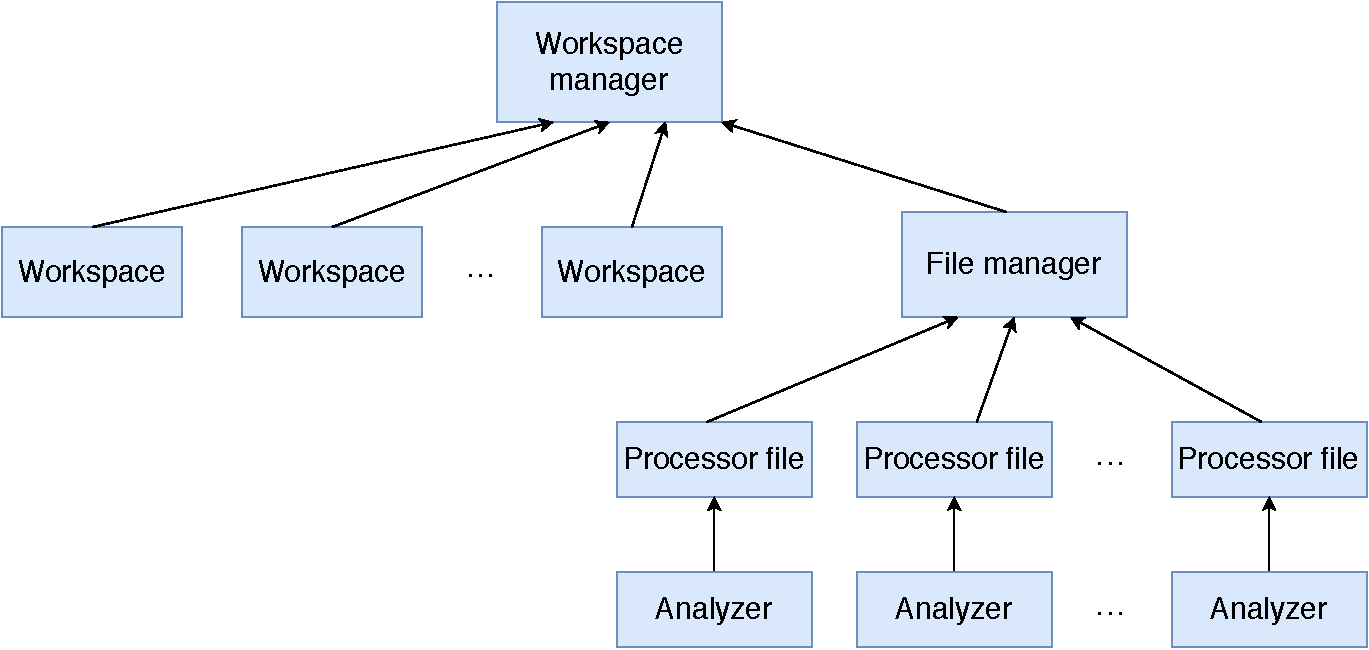
\includegraphics[width=\textwidth]{img/diagnosable_hierarchy}
	\caption{Hierarchy of diagnostics collection in the workspace manager component}
	\label{diagnosable_hierarchy}
\end{figure}

\chapter {Analyzer}
\label{chap:analyzer}

The role of the analyzer is to provide a facade over objects and methods to create a simple interface for lexical and semantic processing (analyzing) of a single HLASM source file. The output of the analysis is the basic input of the LSP server.


After the analyzer is constructed, it analyzes the provided source file. As a result, it updates HLASM context tables and provides a list of diagnostics linked to the file, highlighting, list of symbol definitions, etc.


\sectionSrc{Overview}
{parser\_library/src/analyzer.h}

The analyzer is composed of several sub-components, all required to properly process the file. 
\begin{description}
	\item[LSP data collector] collects and retrieves all LSP information created while processing the file.
	\item[HLASM context tables] hold information about the context of the processed HLASM source code.
	\item[Lexer--Parser sub-components] simplify the processing interface and ease the use of this component. They are needed to create a source file parser.
	\item[Processing manager] executes the main loop where the file is processed.
\end{description}

LSP data collector is required by Lexer-Parser sub-components. They are composed into the parser object required by processing manager. HLASM context tables are used by the manager and the sub-components as well. 

The components together contribute to the proper functionality of the method \TT{analyze}. It processes a provided file and fills LSP data collector from which LSP information can be further retrieved.  

\subsection{Construction}

In order to parse a HLASM file, the analyzer class is constructed with the following parameters:
\begin{itemize}
	\item \emph{Name and content of a file.}
	\item \emph{Parse library provider} -- an object responsible for resolving source file dependencies. The dependencies are only discovered during the analysis, so it is not possible to provide the files beforehand.
	\item \emph{Processing tracer} (see \cref{macro_tracer}).
\end{itemize}

When this constructor is used, the analyzer creates HLASM context tables and processes the provided source as an open-code. We say that the analyzer has \emph{owner semantics}; it is the owner of the context tables. 
 
The analyzer provides \emph{reference semantics} as well (holding just a reference of the context tables). The provided source is not treated as an open-code, rather as an external file dependency. The constructor of an analyzer with reference semantics adds the following two parameters to the previous one:
\begin{itemize}
	\item \emph{HLASM context tables reference} --- belongs to the owning open-code analyzer.
	\item \emph{Library data} --- states how the dependency file should be treated (see \cref{lab06:lib_data}).
\end{itemize}

This constructor is called within open-code analyzer by its sub-components when they use the \emph{Parse library provider}.


\sectionSrc{LSP data collector}
{parser\_library/src/semantics/lsp\_info\_processor.h}
\label{lsp_data}

The data collection is necessary to be able to reply to the LSP requests without the need to re-parse. During the parsing process, a component called \emph{LSP info processor} processes and stores this information. The main goal of this component is to collect as much information as possible to provide meaningful and complex replies to the LSP requests while maintaining the memory and parse-time overhead negligible.

\emph{LSP info processor} is invoked after each parsed and processed statement to collect and store the information it needs inside the \emph{LSP context} (part of HLASM context). 

\subsection{Supported LSP language features}
The plugin implements four LSP language features:
\begin{description}
	\item[hover] The \emph{hover} feature is invoked whenever a user moves his mouse cursor over a symbol for a short period of time. Typically a box with the information about the selected symbol appears right next to it.
	\item[complete] The \emph{complete} feature may be triggered by a custom set of events such as typing a specific character. The server responds with a list of possible correct options that can be inserted into the particular position.
	\item[go\_to\_definition] The \emph{go\_to\_definition} feature is invoked manually from the editor by selecting a symbol and consequently invoking the \TT{go\_to\_definition} command. The editor "jumps" to the location of the currently selected symbol's definition by moving the cursor to that location.
	\item[references] The \emph{references} feature is invoked in a similar manner as the \emph{go\_to\_definition} feature. But the results of the \emph{references} feature are displayed as a list of all references to the selected symbol in the project, not just the definition of it. 
\end{description}

\subsection{Supported HLASM symbols}
The symbols, on which the user might call mentioned LSP features, are \emph{instruction symbols}, \emph{variable symbols}, \emph{sequence symbols} and \emph{ordinary symbols}.

The \emph{references} and the \emph{go\_to\_definition} features are very similar for each symbol type and in most cases work as described above. 

However, there are two exceptions to the standard behavior of the \emph{go\_to\_definition} feature.
First, the command jumps to the definition of an instruction symbol only for macros (to the macro definition file). For the built-in instructions, the feature simply jumps to the first occurrence of the instruction. Second, the command used on an ordinary COPY symbol jumps to the corresponding copy file.

On the other hand, the responses to the \emph{hover} and the \emph{complete} features vary for each symbol type and are described in the following tables:
\begin{table}[h]
	\centering
	\begin{tabular}{ll}
		\toprule
		\textbf{Symbol Type}            & \textbf{Hover contents}                              \\ \midrule
		\multirow{2}{4cm}{instruction}  & the type of the instruction, the syntax of its parameters \\ 
		                                & the version (macros only), the documentation \\ \midrule
		variable                        & the type of the variable --- bool/string/number       \\ \midrule
		sequence                        & the position of the definition                \\ \midrule
		ordinary                        & absolute/relocatable, the value, the values of attributes \\
		(COPY)                          & the name of the copy file                               \\  
		\bottomrule
	\end{tabular}
	\caption{The contents of the \emph{hover} feature for each symbol type.}
\end{table}

\begin{table}[h]
	\centering
	\begin{tabular}{lll}
		\toprule
		\textbf{Symbol Type}            & \textbf{Trigger Characters, Events}     & \textbf{Response}  \\ \midrule
		\multirow{2}{3cm}{instruction}  &  A-Z,@,\$,\# after any number of spaces & built-in HLASM instructions\\ 
	                                   	& from the start of the line              & + already used macros     \\ \midrule
		\multirow{3}{3cm}{variable}     & \multirow{3}{4cm}{\&}                   & variable symbols defined \\ 
	 	                                &                                         & before the current line  \\ 
	 	                                &                                         & in the current scope \\ \midrule
		\multirow{2}{3cm}{sequence}     & \multirow{2}{4cm}{.}                    & sequence symbols defined \\ 
										&                                         & before the current line  \\ \midrule
		ordinary                        & \textit{not implemented}                & \textit{not implemented} \\
		\bottomrule
	\end{tabular}
	\caption{The trigger event and the reponse to the \emph{complete} feature for each symbol type.}
\end{table}




\sectionSrc[.5\linewidth]{Processing manager}{parser\_library/src/processing/processing\_manager.h}
\label{chap:process}
Processing manager is a major component in the processing of a HLASM source file. It decides which stream of statements is to be processed and how statements are going to be processed. It contains components responsible for instruction interpretation as well as instruction format validation. 

Nature of the HLASM source interpretation requires that various parsers and code generators interlace to implement semantics of all instructions. Processing manager performs this by maintaining 2 sets of active generators ("providers") and consumers (parsers, "processors") and executing them on demand, in an interleaved manner.

\begin{figure}
	\centering
	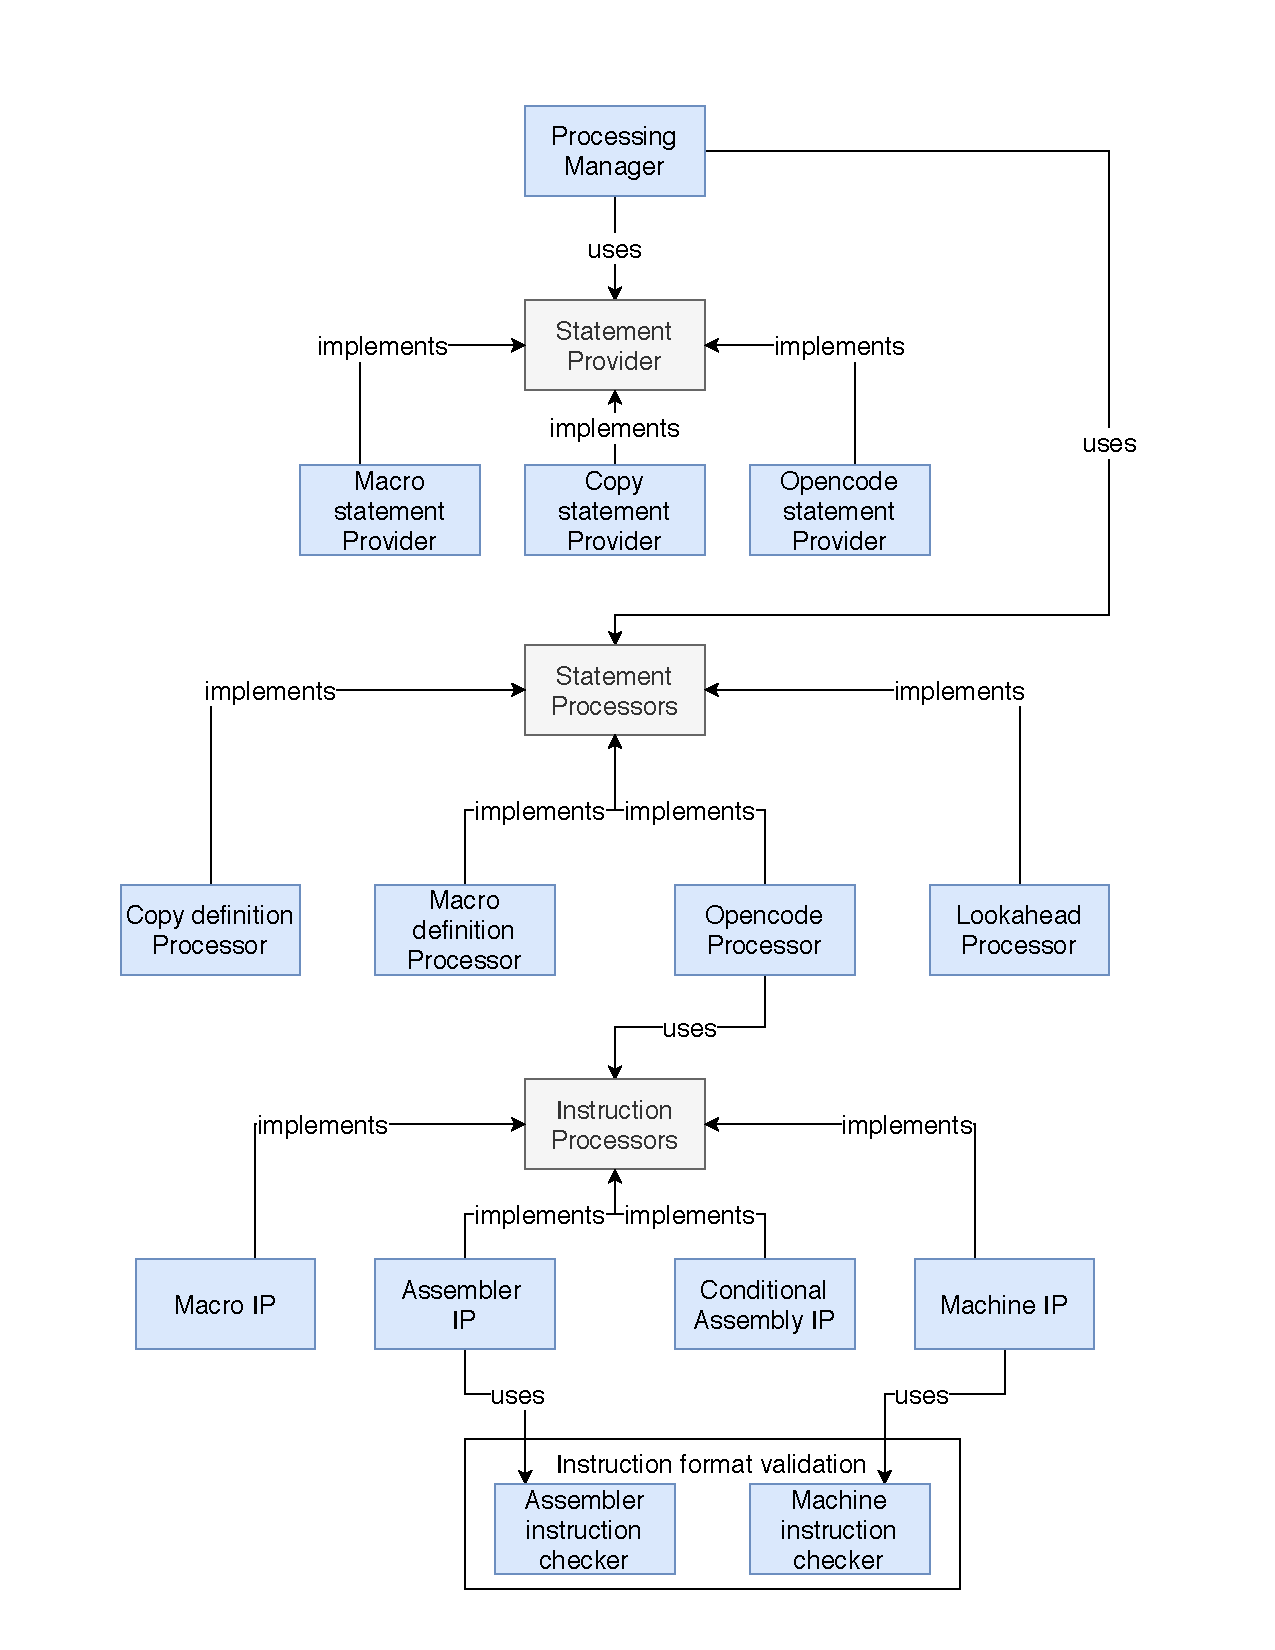
\includegraphics[width=\textwidth]{img/processing_manager_arch}
	\caption{The architecture of Processing manager}
	\label{fig06:proc_mngr}
\end{figure}

\subsection{Overview}

Following objects passed by analyzer serve as an input for the processing manager:
\begin{itemize}
	\item \emph{Parser} that provides statements from the processed file. Further on in this chapter, we will refer to the parser as to the \emph{Opencode statement provider}.
	\item \emph{HLASM context tables} that hold current state of the parsed code.
	\item \emph{Library data} defining the initial state of the manager (whether the file is copy member, macro definition, etc.; see \cref{lab06:lib_data}). 
	\item \emph{Name} of the processed file.
	\item \emph{Parse library provider} to solve source file dependencies.
	\item \emph{Statement fields parser} for parsing yet unresolved statement fields. 
	\item \emph{Processing tracer} for tracing processed statements (see \cref{macro_tracer}).
\end{itemize}


\subsection{Composition}

As the processing of the HLASM source file is rather complicated, we define a complex set of abstraction objects over the complicated assembling of HLASM language:

\begin{description}
	\item[Statement provider] (see \cref{lab06:sect_prov}) is able to produce \TT{statement} structures. Its functionality is to provide statements from its various statement sources (e.g., a source file for Opencode provider, a macro/copy definition for Macro/Copy provider).
	
	\item[Statement processor] (see \cref{lab06:sect_proc}) is an object that takes statement structures from a provider. Then, it performs a specific action with the acquired statement; namely, stores it into macro/copy definition (\emph{Macro/Copy processor}) or looks for sequence symbol (\emph{Lookahed processor}) or performs contained instruction (\emph{Opencode processor}).
	
	\item[Instruction processors] (see \cref{lab06:instr_proc}) help opencode statement processor in performing actions with the instructions contained in a statement. Each one of four instruction processors (Macro, Assembler, Machine and Conditional Assembly IP) processes separate sub-set of a broad set of HLASM instructions. 
	
	\item[Instruction format validators] (see \cref{checker}) are used by instruction processors. As an input, they take operands of an instruction and serve to validate their correctness. 
	
\end{description}

Processing manager encapsulates above mentioned objects and determines which processor/provider will be used next (see \cref{fig06:proc_mngr}).


\subsection{The main loop of manager}
\label{lab06:mngr_loop}

Processing manager contains an array of active statement processors and an array of active statement providers. It is in the control of which processor--provider pair currently operates.

The main processing loop works with the currently operating processor and provider. In the loop body, statement provider provides next statement for statement processor that processes it accordingly. The loop breaks when all processors finish work and none of them is active.

When provider ends its statement stream or processor finishes its work, it is replaced with another. The following rules apply:

\begin{enumerate}
	\item When a processor finishes its work, the next processor is selected from the array.
	\item When a provider finishes --- before the next provider is selected from the array~--- manager checks whether it triggers the termination of the current processor as well (see \emph{terminal condition} in \cref{lab06:sect_proc}). If true, perform rule 1, otherwise the current processor stays active.
\end{enumerate}

\subsection{Initial state of manager}
\label{lab06:lib_data}

During initialization, the manager sets various statement providers and processors as a default. It is very important as it determines the way how the source is processed. The manager determines this from \emph{library data} passed by analyzer.

Library data contain a file name and an enumeration indicating a kind of the file that is being parsed --- \emph{processing kind}.

\emph{Ordinary} processing kind states that the file being processed is the main source file (in HLASM called open-code). It is the first file to be processed. With this information, manager initializes all statement providers and \emph{only} opencode processor. This initial state is applied when analyzer has owner semantics.

\emph{Copy} and \emph{Macro} processing kinds state that manager will process source code that contains copy or macro definition respectively. Hence, \emph{only} copy definition processor or macro definition processor is initialized. Also, all statement providers but the macro statement provider are initialized as no macros will be visited nor needed as a statement source when processing new source code. The library data is passed when analyzer has reference semantics.



\subsectionSrc{Statement Processors}{parser\_library/src/processing/statement\_processors/statement\_processor.h}
\label{lab06:sect_proc}

The motivation for distinguishing different statement processors was the complexity of HLASM language. There are many cases when the same statements require different processing under different circumstances (e.g. COPY instruction in macro is handled differently than in opencode, or lookahead mode can accept statements that would fail when processed by ordinary processing).

During processing, statement processing kinds can be nested. Hence, statement processors are dynamically assigned to the manager when needed and removed from it when they finish. This happens when the processor encounters specific statement (e.g. statement with a special instruction or non previously defined sequence symbol, see \cref{tab06:processor_change}). For this purpose, they use \emph{processing state listener} interface (implemented by processing manager) that tells the manager to change the current processor.

\subsubsectionSrc{Statement structure}{parser\_library/src/context/hlasm\_statement.h,parser\_library/src/processing/statement.h,parser\_library/src/semantics/statement.h}
Statement consists of \emph{statement fields} --- \emph{label field}, \emph{instruction field}, \emph{operands field}, \emph{remark field}. It is used by statement processors and produced by statement providers. 

The abstract class \emph{HLASM statement} is the ancestor for all statement related classes. Then, there are abstract classes \emph{deferred statement} and \emph{resolved statement}. Deferred statement has its operand field stored in uresolved --- deferred --- format (in code stored as string). This statement is created when actual instruction is not yet known prior to the statement creation (see \cref{lst:def_stmt}). Resolved statements are complementary to the deferred statements as their instruction --- as well as operand format --- is known prior to the statement creation.

\begin{listing}[t]
	\begin{Verbatim}[commandchars=\\\{\},codes={\catcode`$=3}]
*VALUE OF INSTRUCTION IN DEFERRED STATEMENT IS PARAMETER OF MACRO MAC
     MACRO
     MAC      &INSTR
     &INSTR   3(2,0),13      $\leftarrow\normalfont\text{deferred statement}$
     MEND
	\end{Verbatim}
	\caption{An example of deferred statement in code.}
	\label{lst:def_stmt}
\end{listing}




\subsubsectionSrc{Copy and Macro definition Processors}
{parser\_library/src/processing/statement\_processors/copy\_processor.h,parser\_library/src/processing/statement\_processors/macrodef\_processor.h}

Both of these statement processors handle statement collecting, forming definition structure and storing it into HLASM context tables. They come into effect when COPY instruction or macro definition is encountered in the source code. 

The statements collected inside copy or macro definitions are mainly deferred statements. That is because variable symbols can not be resolved inside the definition and because HLASM allows instruction aliasing (renaming instructions). Therefore, during the processing of a definition, as the instruction field is parsed, the format of its operands is unknown. It is fully deduced when the definition is handed over to the provider and processed by the opencode processor.

However, some statements in the macro and copy definitions forbid aliasing and the operand format can be deduced immediately (e.g. conditional assembly instructions in macro definition). This leads to the processors necessity to ask the provider to retrieve the statement with correct format -- accordingly to the deduced one based on the instruction being provided  (see \cref{lab06:proc_stat}).

\subsubsectionSrc{Lookahead Processor}
{parser\_library/src/processing/statement\_processors/lookahead\_processor.h}
\label{lab06:look}
Lookahead processor is activated when currently processed conditional assembly statement requires a value of undefined ordinary or sequence symbol. It looks through the succeeding statements and finishes when the target symbol is found or when all statement providers finish. Then the processing continues from where the lookahead started.

\subsubsectionSrc{Opencode Processor}
{parser\_library/src/processing/statement\_processors/ordinary\_processor.h}
\label{ord_proc}
The functionality of Opencode processor (\texttt{ordinary\_processor} class) can be described as follows:
\begin{enumerate}
	\item If a model statement is encountered (see \cref{var_sym}), it substitutes the variable symbols and resolves the statement.
	\item It checks statement for validity.
	\item It performs instruction by updating HLASM context tables with the help of \emph{instruction processors}.
	\item It is passed \emph{processing tracer} by the manager. Each time a statement is processed by opencode processor, it triggers processing tracer. The tracer serves as a listener pattern used by \emph{Macro tracer} (see \cref{macro_tracer}).
\end{enumerate}

\vspace{0.5cm}

In the \cref{tab06:processor_change}, we can see that it does not have a field that starts Opencode processor. That is because this processor is set as a default by the manager. Further, Copy processor does not finish itself during its work as it can only be finished by its \emph{terminal condition} (see \cref{tab06:term_cond}). 

Terminal condition can be triggered by a finishing provider. It indicates that the processor needs to finish its work when a specific provider exhausted its statement stream.

\newcommand{\fin}{\textcolor{red}{finish}}
\newcommand{\strt}[1]{\textcolor{blue}{start #1}}
\newcommand{\cont}{\textcolor{green}{continue}}

\begin{table}
	\centering
	\begin{tabular}{@{}p{0.17\textwidth}ccccc@{}}
		\textbf{Processor} & \thead{\textbf{END}\\ \textbf{instruction}} & \thead{\textbf{COPY}\\ \textbf{instruction}} & \thead{\textbf{MACRO}\\ \textbf{instruction}} & \thead{\textbf{MEND}\\ \textbf{instruction}} & \thead{\textbf{undefined} \\ \textbf{symbol}} \\ \toprule
		\textbf{Opencode}  &                    \fin                     &                 \strt{Copy}                  &                 \strt{Macro}                  &                    \cont                     &               \strt{Lookahead}                \\
		\textbf{Copy}      &                    \cont                    &                    \cont                     &                     \cont                     &                    \cont                     &                     \cont                     \\
		\textbf{Macro}     &                    \cont                    &                 \strt{Copy}                  &                     \cont                     &                     \fin                     &                     \cont                     \\
		\textbf{Lookahead} &                    \fin                     &                 \strt{Copy}                  &                     \cont                     &                    \cont                     &                     \cont                     \\ \bottomrule
	\end{tabular}
	\caption{Description of statement processor changes.}
	\label{tab06:processor_change}
\end{table}

\subsectionSrc{Statement Providers}
{parser\_library/src/processing/statement\_providers/statement\_provider.h}
\label{lab06:sect_prov}

Due to the macro definitions, copy file includes and statement generation, it is difficult to state which statement should be processed next. For this reason, we define abstraction over various sources of statements called \emph{statement providers}.

In contrary to statement processors, statement providers are ordered based on the priority (lower index, greater priority):

\begin{enumerate}
	\item Macro definition statement provider
	\item Copy definition statement provider
	\item Opencode statement provider
\end{enumerate}

In each iteration of processing manager (see \cref{lab06:mngr_loop}), providers are asked whether they have statements to provide based on the ordering. That is because after each iteration, a provider with greater priority than the previously used one can be activated. 


\begin{table}
	\centering
	\begin{tabular}{@{}p{0.20\textwidth}ccc@{}}
		\textbf{Processors} & \thead{\textbf{Macro provider} \\ \textbf{ends}} & \thead{\textbf{Copy provider} \\ \textbf{ends}} & \thead{\textbf{Opencode provider} \\ \textbf{ends}} \\ \toprule
		\textbf{Opencode}   &                      \cont                       &                      \cont                      &                        \fin                         \\
		\textbf{Copy}       &                      \cont                       &                      \cont                      &                        \fin                         \\
		\textbf{Macro}      &                       \fin                       &                      \cont                      &                        \fin                         \\
		\textbf{Lookahead}  &                       \fin                       &                      \cont                      &                        \fin                         \\ \bottomrule
	\end{tabular}
	\caption{Description of statement processors' terminal condition.}
	\label{tab06:term_cond}
\end{table}

For the main loop to be correctly defined, the end of opencode provider triggers terminal condition for all statement processors. Hence, when opencode provider finishes then all the processors finish as well and the processing ends (see \cref{tab06:term_cond}).

\subsubsection{Statement passing}
\label{lab06:proc_stat}

In HLASM language, it is difficult to parse statements into one common structure due to its \emph{representational ambiguity}; the major difference between operand fields of different instruction formats. Moreover, when parsing statements, the instruction format can be yet unknown. Therefore, operand fields are stored as strings. This means that during statement passing when instruction format is deduced, the provider has responsibility to produce correct statement format. The following steps are applied in the statement passing (also see \cref{fig06:process_next}):

\begin{enumerate}
	\item Provider retrieves the instruction field part of the statement.
	\item Provider calls processor method \texttt{get\_processing\_status} with instruction field as a parameter.
	\item Return value of the call determines the required format of the operand field for the processor; the whole statemement can be retrieved correctly.
	\item Provider returns statement with correct format to the processor. 
\end{enumerate}

\begin{figure}
	\centering
	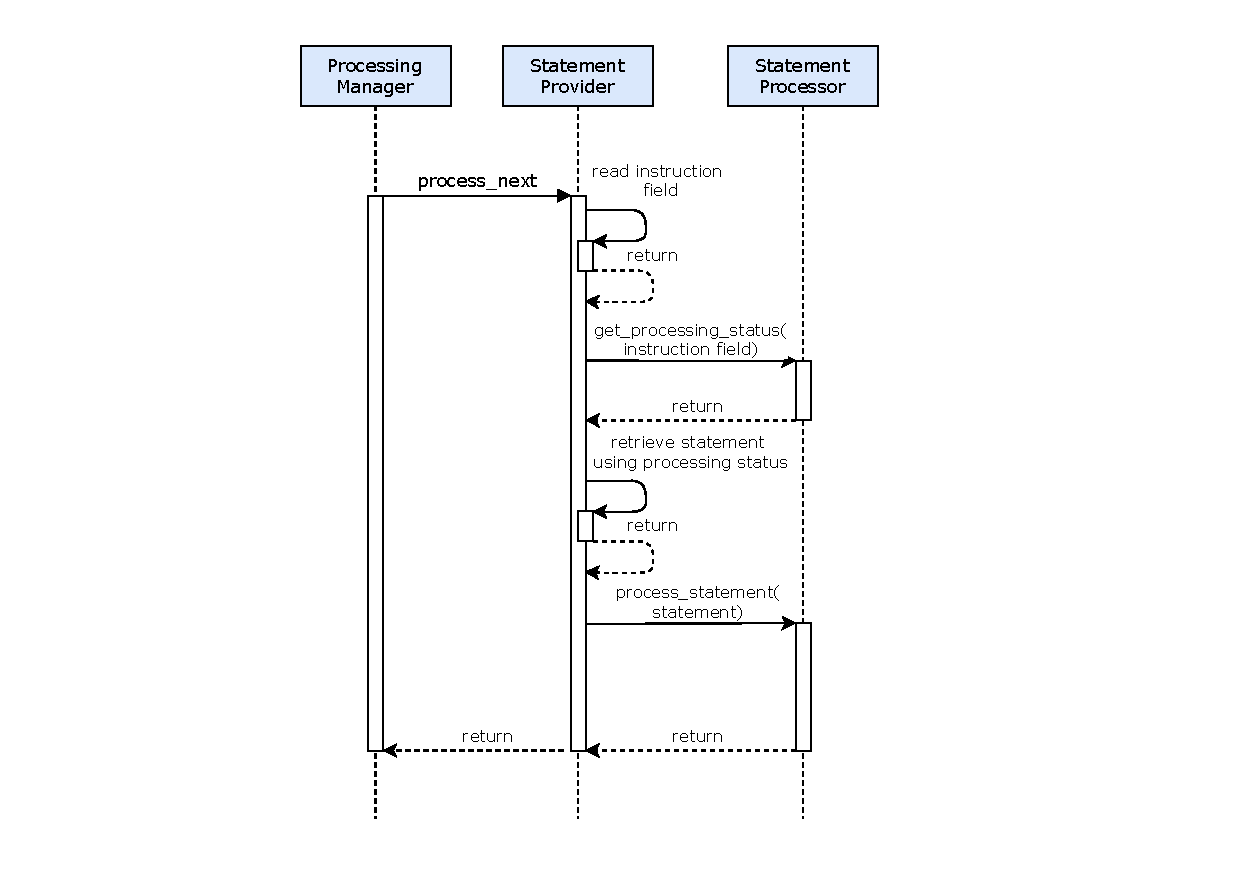
\includegraphics[width=13cm]{img/process_next}
	\caption{The process of statement passing.}
	\label{fig06:process_next}
\end{figure}


\subsubsectionSrc{Copy and Macro definition Provider}
{parser\_library/src/processing/statement\_providers/copy\_statement\_provider.h,parser\_library/src/processing/statement\_providers/macro\_statement\_provider.h}

These providers are activated when COPY instruction copies a file into the source code or when a macro is visited, respectively. They provide a sequence of statements to an arbitrary processor until all statements from the copy or macro definition are provided. After that, if there is no nested invocation, a provider with lower priority is selected.

To avoid infinite macro recursion, HLASM language itself has a restriction for the level of nested macro invocation depending on the complexity of nested macros. We set the limit to 100 as it suffices in all tested code.

For COPY members, recursion is forbidden.

\subsubsectionSrc{Opencode Provider}
{parser\_library/src/processing/opencode\_provider.h,parser\_library/src/parsing/parser\_impl.h}

Opencode provider is active as long as there are statements in the source file. It retrieves statements from the source code with help of lexer and parser (see \cref{lab06:parser}).

\subsectionSrc{Statement field parser}
{parser\_library/src/processing/statement\_fields\_parser.h}
\label{lab06:field_parser}

Statement field parser is an interface passed to the statement providers by processing manager. It is implemented by the parser (see \cref{lab06:parser}).

At first, it is used during statement passing. In some cases provider is requested a specific format of a string-stored statement. The string is re-parsed with the according format. Then the field is returned back to the statement provider. 

Another use of field parser is in opencode processor as model statements are resolved there. After variable symbol substitution, the resulting string field is re-parsed with field parser.

\subsectionSrc{Instruction processors}
{parser\_library/src/processing/instruction\_sets}
\label{lab06:instr_proc}

Opencode processor divides processing of HLASM instruction types into several \emph{instruction processors}. Each processor is responsible for processing instructions that belong to one instruction type.

As a format of some instruction kinds can be rather complicated, instruction processors contain \emph{Instruction format validators} (see \cref{checker}). They check the statement to validate the correctness of used operand format as well as the correctness of the actual operand values.

During the instruction processing, processors work with HLASM \emph{expressions} (see \cref{ca_expr:logic}, \cref{mach_expr}). They need to be evaluated to correctly perform the processing.

There are four specialized instruction processors:
\begin{description}
	\item[Macro IP] looks up for macro definition in HLASM context tables and calls it.
	\item[Assembler and Machine IP] processes assembler and machine instructions (see \cref{asm_instrs} \cref{mach_instr}) to retain consistency in HLASM context tables.
	\item[Conditional assembly IP] executes conditional assembly instructions (see \cref{ca_instr}). 
	
\end{description}

See the current list of processed instruction in \cref{tab06:instr_proc}.

\begin{table}
	\centering
	\begin{tabular}{lr}
		\textbf{IP}                   &                  \textbf{Processed instructions} \\ \toprule
		\textbf{Assembler}            & *SECT, COM, LOCTR, EQU, DC, DS, COPY, EXTRN, ORG \\
		\textbf{Machine}              &        \emph{Instruction format validation only} \\
		\textbf{Macro}                &                                       \emph{ANY} \\
		\textbf{Conditional Assembly} &    SET*, GBL*, ANOP, ACTR, AGO, AIF, MACRO, MEND \\ \bottomrule
	\end{tabular}
	\caption{Table of instructions that are processed by instruction processors.}
	\label{tab06:instr_proc}
\end{table}

\vspace{0.5cm}

HLASM differentiates two kinds of expressions: \emph{Conditional Assembly} (CA) and \emph{Machine} expressions. CA expressions appear in conditional assembly, which is processed during compilation. Machine expressions are used with assembler and machine instructions.

\subsubsectionSrc[0.5\linewidth]{CA Expressions}
{parser\_library/src/expressions/expression.h,parser\_library/src/expressions/arithmetic\_expression.h,parser\_library/src/expressions/character\_expression.h,parser\_library/src/expressions/keyword\_expression.h,parser\_library/src/expressions/logic\_expression.h,parser\_library/src/expressions/numeric\_wrapper.h}
\label{ca_expr:logic}

HLASM evaluates CA expressions during assembly generation. For further details, refer to the \cref{ca_instr}.

We employ the ANTLR 4 Parse-Tree Visitors during the expression evaluation. For further detail on ANTLR, refer to \cref{antlr}.

In this section, we address the representation and functionality of the expressions themselves. Coupling the expressions with grammar and their evaluation in context is further discussed in \cref{ca_expr:eval}.

HLASM CA expression is conceptually similar to the expressions in other languages: they support unary and binary operators, functions, variables and literals. Evaluation of expressions is further reviewed in \cref{ca_expr:eval}. In HLASM, each expression has a type. \emph{Arithmetic}, \emph{Logic}, \emph{Character} expressions are supported. We implement the logic in the following classes:

\begin{description}
	\item[\texttt{expression}] A pure virtual class that defines a shared interface, operators, and functions. The class also implements evaluation logic for terms and factors.
	
	\item[\texttt{diagnostic\_op}] The concept of \emph{diagnostics} is fundamental. During the evaluation of an expression, an error can occur (syntactic or semantic). Hence, we try to improve the user experience by reporting diagnostics. Each instance of \texttt{expression} has a pointer to \texttt{diagnostic\_op} associated to it. If the pointer is \texttt{null}, it is considered error-free. During the evaluation of a child expression, the parent checks for errors and propagates the error upwards. Checking and propagating of an error is implemented by \texttt{copy\_return\_on\_error} macro, which one should call immediately before the creation of a new expression during evaluation.
	
	The \texttt{expression} class implements the evaluation as follows:
	A \texttt{std::deque} of \texttt{expression} pointers is passed. The evaluation iterates the list from left to right.  Functions, binary, and unary operators consume the rest of the deque.
	
	Some expression symbols can be either HLASM keywords or variable identifiers (see example in \cref{lst:example_ca_expr}). Therefore, the resolution of symbols is complicated and cannot be done straight, but instead during the evaluation-time. The order of the expression's terms and the previous evaluation context is crucial for the disambiguation. 
	
	\item[\texttt{keyword\_expression}] Helper class that represents HLASM keywords in expressions. It determines a keyword type from a string, containing its arity (unary, binary) and priority.
	
	\item[\texttt{logic\_expression}] Represents a boolean expression.
	
	\item[\texttt{arithmetic\_expression}] Represents an arithmetic expression.
	
	\item[\texttt{arithmetic\_logic\_expr\_wrapper}] HLASM language supports expressions with operands of mixed types. For more straightforward and readable use of arithmetic and logical expressions, this class wraps them under one class.
	
	\item[\texttt{character\_expression}] Represents a character expression.
	
	\item[\texttt{ebcdic\_encoding}] This class defines a custom EBCDIC literal and provides helper functions for conversion between EBCDIC and ASCII. EBCDIC is a character encoding used in the IBM mainframe. It has a different layout than ASCII.
	
	\item[\texttt{error\_messages}] It is a static class with list of all \texttt{diagnostic\_op} that can be generated from expressions.
	
	
\end{description}

\iffalse
\begin{lstlisting}[label={ca_expr:example},language=C++,backgroundcolor=\color{cyan!10}, captionpos=b, caption=Defition of \texttt{copy\_return\_on\_error} macro and an example of its usage while evaluating unary expression \texttt{B2A("123")}. \texttt{this} is an \texttt{character\_expression} with value \texttt{"123"}.]
#define copy_return_on_error(arg, type) \
do \
{ \
auto te = test_and_copy_error<type>(arg); \
if (te != nullptr) return te; \
} \
while(0)

//before upward propagating the operation result
//call the macro
copy_return_on_error(this, arithmetic_expression);
return arithmetic_expression::from_string(value_, 2);

\end{lstlisting}
\begin{figure}
	\centering
	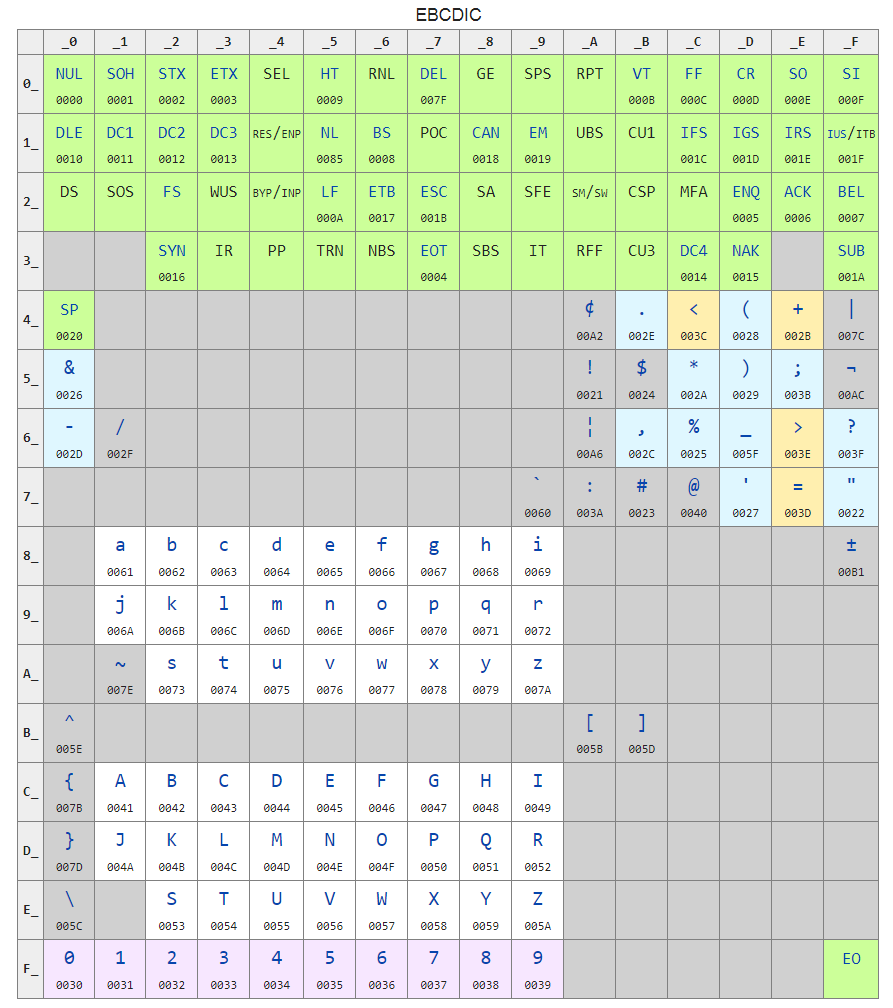
\includegraphics[height=13cm]{img/ebcdic}
	\caption{EBCDIC layout. Taken from \url{https://i.stack.imgur.com/h3u5A.png}.}
	\label{ca_expr:ebcdic}
\end{figure}
\fi

\begin{listing}[t]
	\begin{verbatim}
    name        operation   operands
	
    AND         EQU         1
    NOT         EQU         0
                AIF         (NOT AND AND AND).LAB   < EVALUATES TO (!1 & 1)
	\end{verbatim} 
	\caption{An example of using keywords (\texttt{AND} and \texttt{NOT}) as variable names resulting in a confusingly valid expression (line 3).}
	\label{lst:example_ca_expr}
\end{listing}

\subsubsectionSrc{CA expression evaluation}
{parser\_library/src/expressions/visitors/expression\_analyzer.h,parser\_library/src/expressions/visitors/expression\_evaluator.h,parser\_library/src/expressions/evaluation\_context.h}
\label{ca_expr:eval}

In the previous section, we described the representation of the CA expressions themselves. In this section, we explain the coupling of CA expressions with grammar via visitor. 

The \texttt{expression\_evaluator} encapsulates the coupling logic between the grammar and the expression logic. That is, the evaluator has a notion about grammar, which translates into C++ expression logic.

The top-level expression first gathers a list of space-separated expressions. The evaluation must be done using a list from left to right (not using a tree) as any token may be a keyword (such as \texttt{AND} operator) or variable identifier, depending on a position in an expression (using language keywords as identifiers is allowed in HLASM). For a better understanding, see \cref{lst:example_ca_expr}. \texttt{expression::evaluate} provides the disambiguation (see \cref{ca_expr:logic}). 

During its work, evaluator substitutes variable and ordinary symbols for their values. To know which values to substitute, evaluator is given \emph{evaluation context}. It consists of objects that are required for correct evaluation: \emph{HLASM context} for symbol values, \emph{attribute provider} for values of symbol attributes that are not yet defined and \emph{library provider} for evaluation of some types of symbol attributes as well.

Lookahead (see \cref{lab06:look}) is triggered in conditional assembly expressions when evaluation visits yet undefined ordinary symbol. As this can be rather demanding operation, expression evaluator uses \emph{expression analyzer}. It looks for all the undefined symbol references in expression and collects them to a common collection. Then, the lookahead is triggered to look for all references in the collection. Hence, it is triggered once per expression rather than any time an undefined symbol reference is found. 

\subsubsectionSrc[0.45\linewidth]{Machine expressions}
{parser\_library/src/expressions/mach\_expression.h,parser\_library/src/expressions/mach\_expr\_term.h,parser\_library/src/expressions/mach\_operator.h}
\label{mach_expr}

In HLASM, machine expressions are used as operands of machine and assembler instructions. Their result may be a simple absolute number or an address.

We use a standard infix tree representation of expressions. There is an interface \TT{machine\_expression} which is implemented by several classes that represent operators and terms. Each binary operator holds two expressions --- left and right operands. Terms are leaf classes that do not hold any other expressions and directly represent a value. There are several classes representing different terms valid in machine expressions:
\begin{itemize}
	\item \TT{mach\_expr\_constant} represents simply a number.
	\item \TT{mach\_expr\_symbol} represents an ordinary symbol.
	\item \TT{mach\_expr\_data\_attr} represents attribute of a symbol (e.g. \TT{L'SYM} is length of symbol \TT{SYM})
	\item \TT{mach\_expr\_location\_counter} represents location counter represented by asterisk in expressions. 
	\item \TT{mach\_expr\_self\_def} represents self defining term (e.g. \TT{X'1F'})
\end{itemize}
\Cref{mach_expr_example} shows an example representation for one concrete expression.

\begin{figure}
	\centering
	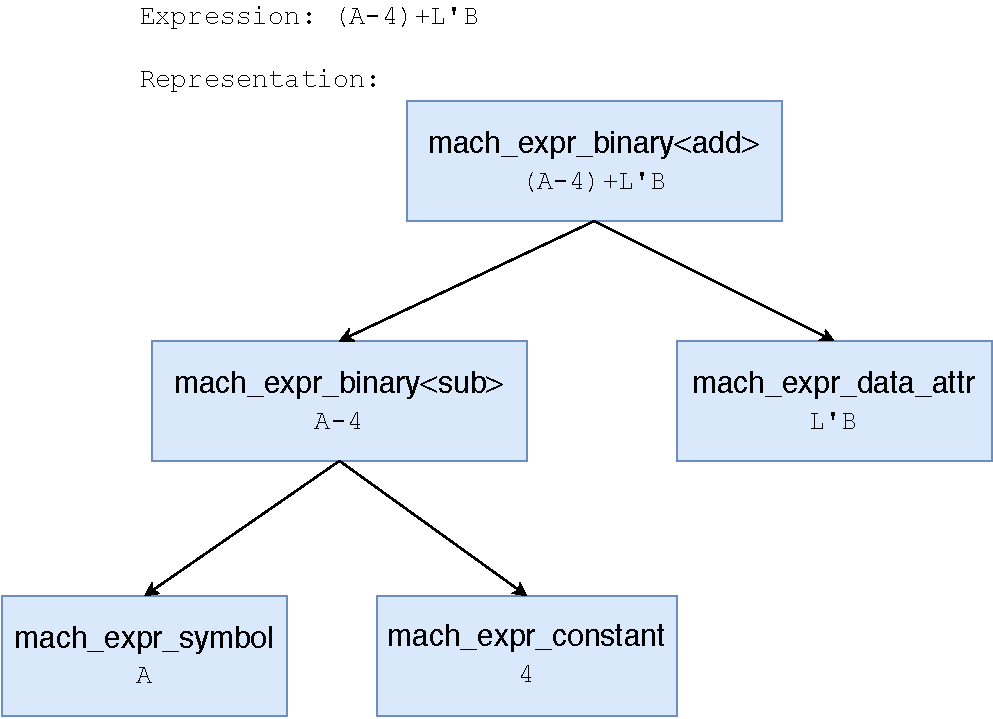
\includegraphics[width=13cm]{img/mach_expr_example}
	\caption{Example representation of the machine expression \TT{(A-4)+L'B}.}
	\label{mach_expr_example}
\end{figure}

Machine expressions are also able to evaluate the expressions they represent. The evaluation is done in a recursive manner. It is fairly simple when there are no symbols used in the expression --- each node in the tree simply computes the result with basic arithmetic operations.

However, the process can get tricky since expressions may contain e.g. \TT{mach\_expr\_symbol} whose value is dependant on symbols defined in other parts of source code. Moreover, result of a machine expression may be an absolute value (a number) or relocatable value (an address). The process of symbols resolution is explained in \cref{symbol_dependency_tables}.

\sectionSrc{Instruction format validation}
{parser\_library/src/context/instruction.h,parser\_library/src/checking/operand.h,parser\_library/src/checking/instr\_operand.h}

\label{checker}
One of the essential ways to provide results of the parsing to the user is through error messages. Many of these messages are created in \emph{Instruction checker} which validates the usage of different kinds of instructions.

Instruction checker is an abstract class for various types of instructions. Its \TT{check} method is being called from the instruction processors~\ref{chap:process} to check whether the specific instruction is used with correct parameters. As assembler and machine instructions have different formats, we derive separate \emph{assembler} and \emph{machine} checkers from the instruction checker. CA instructions do not have a derived checker class as they are all being checked during their interpretation.

The checkers need an access to the definitions of all possible instructions. These instructions are stored statically inside an object called \emph{instruction}. It consists of 4 different containers:
\begin{itemize}
	\item \emph{machine\_instructions} is a map of instruction names to machine instruction object, which contains various data such as format, size or vector of instruction's operands.
	\item \emph{mnemonic\_codes} maps instruction names to their mnemonic code. The mnemonic codes are simplified versions of specific machine instructions, substituting one of the operands by a default value. The mnemonic code objects provides a list of operands to be substituted along with the original instruction name.
	\item \emph{assembler\_instructions} is similar to the machine instructions. However, as the assembler instructions do not have formats, these classes only state minimum/maximum number of operands for specific instruction.~In~\cref{sub:asm_check}, we explain how the assembler instructions are validated.
	\item \emph{ca\_instructions} only contains a list of possible CA instructions.
\end{itemize}

Both assembler and machine checker works in a similar manner:
\begin{enumerate}
	\item Either assembler or machine processor calls the \TT{check} method of its respective checker. This method accepts the instruction name, the vector of used operands, the range of statement and the diagnostic collector.
	\item Checker finds the correct instruction based on the provided name and calls the \TT{check} method of its instruction class, along with the same parameters as mentioned above.
	\item The instruction itself compares its possible operands with the used operands.
	\item More validations may be necessary, based on the instruction.
	\item In case of mismatch, a diagnostic is added to the passed diagnostic container.
\end{enumerate}

\subsectionSrc{Machine instruction checker}
{parser\_library/src/checking/instruction\_checker.h,parser\_library/src/context/instruction.h}

All machine instructions have a precisely defined format which makes the validation based on these formats straightforward. Machine instructions checker operates with machine instructions and their mnemonic codes.

The formats are defined by several basic operands such as register or address and state which combination of these operands are acceptable. For example, instruction LR has format RR, which means it accepts only 2 arbitrary (but correct) registers. 

\begin{figure}
	\centering
	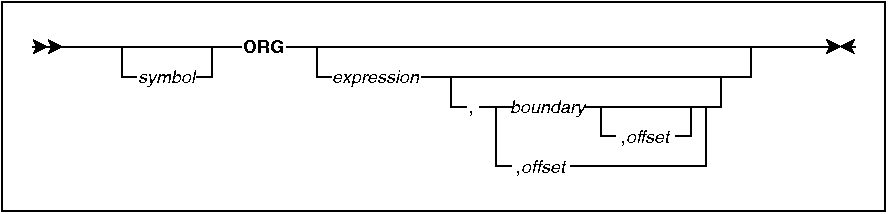
\includegraphics[width=\textwidth]{img/org_diagram}
	\caption{Operand diagram for the ORG instruction.}
	
	\label{fig01:check}
\end{figure}

\subsectionSrc{Assembler instruction checker}
{parser\_library/src/checking/asm\_instr\_class.h,parser\_library/src/checking/asm\_instr\_check.h}
\label{sub:asm_check}

Validation of assembler instructions is more complicated as there are no pre-defined formats for them. Each of them is described by custom operand diagrams, which demonstrate the dependencies and relations between operands of a specific instruction. An example of such diagram for the ORG instruction is shown in \cref{fig01:check}. As an addition to the basic operands used for machine instructions, each assembler instruction might have its own operands, called keywords.

Due to these irregularities, we derive instruction-specific classes from assembler instruction class. Each of them implements the \TT{check} method, to provide the customized checking.

\subsubsectionSrc[0.55\linewidth]{Data Definition checking}
{parser\_library/src/checking/data\_definition/data\_def\_fields.h,parser\_library/src/checking/data\_definition/data\_def\_type\_base.h,parser\_library/src/checking/data\_definition/data\_def\_types.h,parser\_library/src/checking/data\_definition/data\_definition\_operand.h}

Data definition is a type of operand in HLASM. It represents data that is assembled directly into object code (see \cref{asm_instrs}).

Since there are many types of data definition, there is a data definition subcomponent of instruction validation. Whenever any component of the project needs information about a data definition operand, it can use this subcomponent. It analyzes each type of data definition and is able to return its length, attributes and check its validity.

Each type is different and many have special conditions that must be met to be valid. That is why there is an abstract class \TT{data\_def\_type\_base}, which has 38 implementations --- one for each type (including type extensions). The types are then available in a static associative map that maps names of types to their representations.


\sectionSrc{Lexer}
{parser\_library/src/lexing/lexer.h}

Lexer's responsibility is to read source string and break it into tokens --- small pieces of text with special meaning. The most important properties of the lexer:
\begin{itemize}
	\item each token has a location in the source text,
	\item has the ability to check whether all characters are valid in the HLASM source,
	\item can jump in the source file backward and forward if necessary (for implementation of instructions like AGO and AIF). Because of this, it is not possible to use any standard lexing tool, and the lexer has to be implemented from scratch.
\end{itemize}

As previously mentioned, we designed a custom lexer for HLASM. We had a number of reasons to do so. HLASM language is complex. It was first introduced several decades ago and, during this long time, the language was subjected to development. Such a long time period has made the HLASM language complex. Also, it contains some aggressive features, for example, \texttt{AREAD} or \texttt{COPY}, that can alter the source code at parse time.

Conventional lexing tools are most often based on regular expressions. As discussed above, there are several difficulties that one must consider while designing lexer for this particular language. A regular expression-based lexer would be too difficult or even impossible to design\footnote{One could match separate characters from the input and let the parser or semantic analysis deal with some of the described problems. This drastic solution would cost performance, as parsers are usually more performance demanding.}.

\subsection{Source file encodings}
Source code encodings differ for the used libraries. All strings are encoded in \texttt{UTF} as follows:

\begin{description}
	\item[\texttt{UTF-8}] LSP string encoding,
	\item[\texttt{UTF-16}] offsets (positions in source code) in LSP,
	\item[\texttt{UTF-32}] ANTLR 4 source code representation.
\end{description}

\subsectionSrc{Lexer components}
{parser\_library/src/lexing/input\_source.h,parser\_library/src/lexing/token.h,parser\_library/src/lexing/token\_factory.h}

Beside of the custom lexer, we altered ANTLR's classes \texttt{Token}, \texttt{TokenFactory} and \texttt{ANTLRInputStream} (see \cref{antlr}). The reason was to add custom attributes to token that are vital for later stages of the HLASM code analysis (parsing, semantic analyses, etc.). Lexer functionality is implemented in following classes (see \cref{lexer_arch}):

\begin{figure}
	\centering
	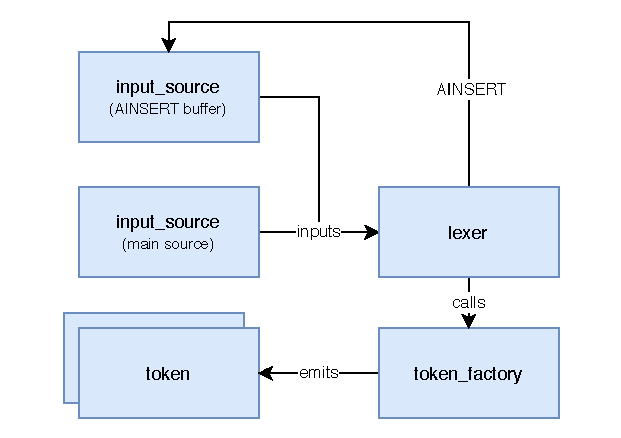
\includegraphics{img/lexer_arch}
	\caption{Lexer architecture overview. Note, there are two \texttt{input\_source}s and there are many \texttt{token}s
		 generated. The \emph{AINSERT buffer} has higher priority. Specifically, if the buffer is non-empty, lexer consumes the input from this buffer. }
	 \label{lexer_arch}
\end{figure}

\begin{description}
	
	\item[\texttt{token}] implements ANTLR's class \texttt{Token} and extends it by adding properties important for location of the token within the input stream. As the LSP protocol works with offsets encoded in \texttt{UTF-16} and ANTLR 4 works with \texttt{UTF-32} encoding, we add attributes for \texttt{UTF-16} positions too.
	
	Token does not carry the actual text from the source but instead references the position in code (unlike \texttt{CommonToken}). Note that the position of a token is vital for further analysis.
	
	\begin{table}
		\centering
		\begin{tabular}{lr}
			\toprule
			\textbf{IGNORED}                                                                     &  sequence of characters ignored in processing \\
			\textbf{COMMENT}                                                                     &                         commentary statements \\
			\textbf{EOLLN}                                                                       &         token signalling the end of statement \\
			\textbf{SPACE}                                                                       &                          a sequence of spaces \\
			\textbf{IDENTIFIER}                                                                  &                             symbol identifier \\
			\textbf{ORDSYMBOL}                                                                   &                    Ordinary symbol identifier \\
			\textbf{PROCESS}                                                                     &                       process statement token \\
			\textbf{NUM}                                                                         &                                        number \\
			\textbf{ATTR}                                                                        & apostrophe that serves as attribute reference \\
			\thead{\textbf{ASTERISK, SLASH, MINUS, PLUS,}\\ \textbf{LT, GT, EQUALS, LPAR, RPAR}} &                             expression tokens \\
			\thead{\textbf{DOT, COMMA, APOSTROPHE,}\\ \textbf{AMPERSAND, VERTICAL}}              &                        special meaning tokens \\ \bottomrule
		\end{tabular}
		\caption{Enumeration of tokens.}
		\label{tab06:tokens}
	\end{table}
	
	Interesting remark of HLASM language complexity is absence of \emph{string} token (see \cref{tab06:tokens}). Lexer does not generate this token due to the existence of model statements (see \cref{var_sym}). There, variable symbol can be written anywhere in the statement (even in the middle of the string), what significantly restricts lexer.
	
	\item[\texttt{token\_factory}] produces tokens of previously described custom type \texttt{token}.
	
	\item[\texttt{input\_source}] implements \texttt{ANTLRInputStream}\footnote{\url{https://www.antlr.org/api/Java/org/antlr/v4/runtime/ANTLRInputStream.html}} which encapsulates source code. This implementation adds API for resetting, rewinding and rewriting input. 
	
	Note the usage of \texttt{UTF} encodings: \texttt{\_data} (source code string) and positions/indices in API are in \texttt{UTF-32}; \texttt{getText} returns \texttt{UTF-8} string.
	
	\item[\texttt{lexer}] is based on ANTLR's \texttt{TokenSource}\footnote{\url{https://www.antlr.org/api/Java/org/antlr/v4/runtime/TokenSource.html}} class. As most lexers, it is also, in principle, a finite state machine. The most important difference compared to conventional FSMs and other lexers is added communication interface that connects the parser and the instruction interpreter with the lexer. Unusual is also input rewinding (to support \texttt{AREAD}, for example), lexing from parallel sources (\texttt{AINSERT} buffer) and some helper API for subsequent processing stages.
	
	Important functions:
	
	\begin{description}
		\item[\texttt{nextToken()}] implements main functionality: lexes and emits tokens. Before lexing, the function uses the right input stream (either the source code or \texttt{AINSERT} buffer if not empty). After choosing the right input source, the lexer emits token. HLASM introduces \textit{continuation} symbol (an arbitrary non-blank symbol in the continuation column) that breaks one logical line into two or more source-code lines. The end of one logical line indicates \texttt{EOLLN} token. Such token is important for further (syntactic and semantic) analysis.
		
		
		\item[\texttt{create\_token()}] creates token of given type. The lexer's internal state gives the position of the token. 
		
		\item[\texttt{consume()}] consumes character from the input stream and updates lexer's internal state (used in \texttt{create\_token()}).
		
		\item[\texttt{lex\_tokens()}] lexing of most of the token types.
		
		\item[\texttt{lex\_begin()}] up to certain column, the input can be ignored (can be set in HLASM).
		
		\item[\texttt{lex\_end()}] lexes everything after continuation symbol.
		
		
	\end{description}
	
\end{description}


\section{Parser}
\label{lab06:parser}

Parser component takes tokens produced by lexer from token stream and recognizes HLASM statements.
The parser inherits from the HLASM recognizer generated by ANTLR (see \cref{antlr}) to provide further operations.

\subsectionSrc{Parser workflow}
{parser\_library/src/parsing/parser\_impl.h,parser\_library/src/semantics/range\_provider.h}

Parser (in code referenced as \TT{parser\_impl}) implements opencode statement provider interface. This means that, according to the statement passing in \cref{lab06:proc_stat}, parser needs to parse each statement in \emph{two steps}:

\begin{enumerate}
	\item Parser calls rule \TT{label\_instr}. It parses label and instruction fields into respective structures. The operand and remark field is stored as a string.
	\item After retrieving the processing format, the parser selects corresponding rule to parse operands. With the rule, it parses remaining string from the previous step.
\end{enumerate}

For the means of parsing remaining strings, parser subcomponent contains actually \emph{two parsers}. The first one parses statement after statement from a source file. The second parses the operands from the string passed by the first parser. 

To achieve operands having correctly set ranges prior to the source file rather than to the passed string, the parser uses \emph{Range provider}. It helps the second parser to have ranges of reparsed operands consistent with the ranges of other fields. It is initialized with the begin location of operand field in the statement and all ranges furtherly created in parsing are adjusted to have correct boundaries.

\subsectionSrc{Statement structure}
{parser\_library/src/semantics/collector.h,parser\_library/src/semantics/statement.h,parser\_library/src/semantics/statement\_fields.h}

During parsing of a statement, several structures are created and collected. They are \TT{label\_si, instruction\_si, operand\_si, remark\_si} (\emph{si} as semantic information). They are collected with \TT{collector} and built into \TT{statement\_si} structure.

Label and instruction structures can contain either identifier of a symbol or --- when in model statement --- concatenation of strings and variable symbols. Remark field is simply just a string as it serves as a commentary statement field. Operand field contains list of operands used in the statement. They can be of several formats.

\subsubsectionSrc{Operand formats}
{parser\_library/src/semantics/operand.h}

The statement processor can request parser to retrieve statements with this operand formats:
\begin{itemize}
	\item \emph{machine/assembler/conditional assembly/macro} -- instruction operands. Each type of instruction has its specific format.
	\item \emph{model} -- operands for model statements. It is a chain of strings and variable symbols.
	\item \emph{deferred} -- operands with not yet known format. Stored as a string.
\end{itemize}

Each operand format has corresponding \emph{operand structure}. They all inherit abstract \TT{operand} and each have various children for different kinds of the operand format (see \cref{fig06:operand_arch}). Assembler and Machine operand structures inherit from \emph{Evaluable operand}. It is a common structure for operand objects that are composed of resolvable objects (see \cref{symbol_dependency_tables}).

\begin{figure}
	\centering
	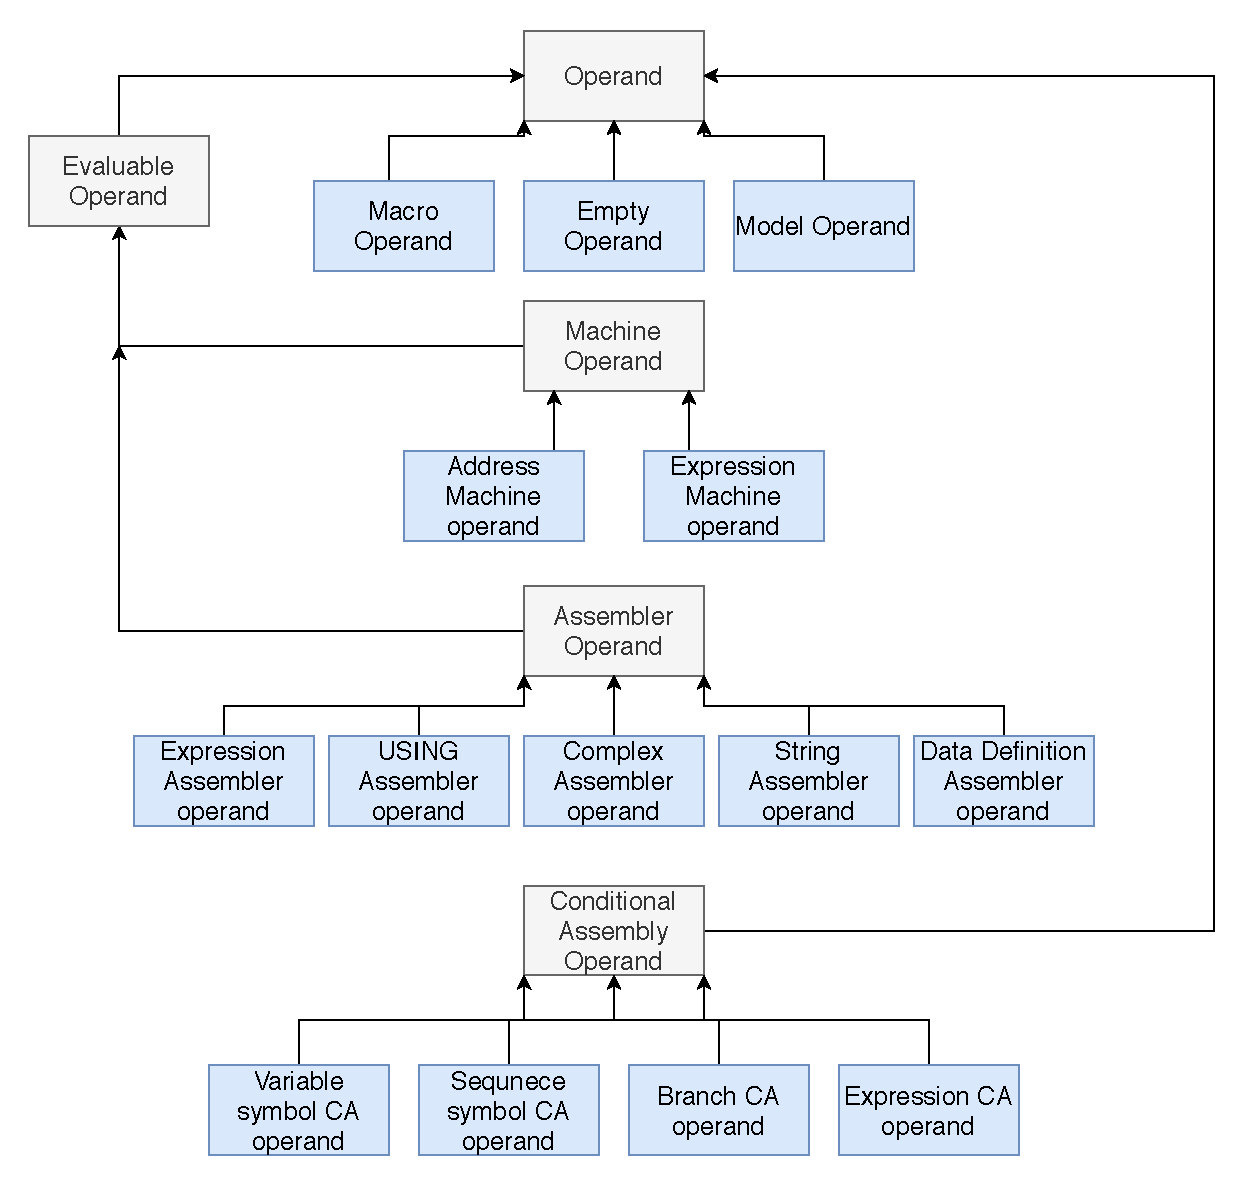
\includegraphics[width=\textwidth]{img/operand_arch}
	\caption{Operand structure inheritance.}
	\label{fig06:operand_arch}
\end{figure}

\subsubsectionSrc{Concatenation structures}
{parser\_library/src/semantics/concatenation.h}

A model statement is a statement that contains a variable symbol in any of the statement fields. This variable symbol is further to be substituted by an arbitrary string and then re-parsed. Hence, the field is formed by concatenating individual sub-fields, which are represented by specialized structures. The concatenation can be further evaluated to produce the final string.

The helper structures are:
\begin{itemize}
	\item \TT{char\_str} -- a character string.
	\item \TT{var\_sym} -- a substitutable variable symbol.
	\item \TT{dot}, \TT{equals} -- characters with special meaning.
	\item \TT{sublist} -- a recursive concatenation enclosed in parentheses.
\end{itemize}

\subsectionSrc{Grammar implementation}
{parser\_library/src/parsing/grammar}

Grammar rules describing parser are separated into several files (see the figure of all grammar rules in \cref{parser_rules}):
\begin{itemize}
	\item \TT{hlasm\_parser.g4} -- Top level rules are stored here.
	\makefileindexnotext{parser\_library/src/parsing/grammar/hlasm\_parser.g4}
	\item \TT{lookahead\_rules.g4} -- Rules for lookahead mode.	\makefileindexnotext{parser\_library/src/parsing/grammar/lookahead\_rules.g4}
	\item \TT{label\_field\_rules.g4} -- Rules taking care of label field of statement. \makefileindexnotext{parser\_library/src/parsing/grammar/label\_field\_rules.g4}
	\item \TT{instruction\_field\_rules.g4} -- Rules taking care of instruction field of statement. \makefileindexnotext{parser\_library/src/parsing/grammar/instruction\_field\_rules.g4}
	\item \TT{operand\_field\_rules.g4} -- Rules taking care of operand field of statement. \makefileindexnotext{parser\_library/src/parsing/grammar/operand\_field\_rules.g4}
	\item \TT{macro/machine/assembler/ca/model/deferred\_operand\_rules.g4} -- Various operand field rules. \makefileindexnotext{parser\_library/src/parsing/grammar/deferred\_operand\_rules.g4}
	\makefileindexnotext{parser\_library/src/parsing/grammar/model\_operand\_rules.g4}
	\makefileindexnotext{parser\_library/src/parsing/grammar/ca\_operand\_rules.g4}
	\makefileindexnotext{parser\_library/src/parsing/grammar/assembler\_operand\_rules.g4}
	\makefileindexnotext{parser\_library/src/parsing/grammar/machine\_operand\_rules.g4}
	\makefileindexnotext{parser\_library/src/parsing/grammar/macro\_operand\_rules.g4}
	\item \TT{ca/asm\_expression\_rules.g4} -- Rules for expressions. \makefileindexnotext{parser\_library/src/parsing/grammar/asm\_expression\_rules.g4}
	\makefileindexnotext{parser\_library/src/parsing/grammar/ca\_expression\_rules.g4}
	\item \TT{data\_def\_rules.g4} -- Rules for data definition. \makefileindexnotext{parser\_library/src/parsing/grammar/data\_def\_rules.g4}
\end{itemize}


\sectionSrc{HLASM context tables}
{parser\_library/src/context/hlasm\_context.h}

HLASM context tables (in code referred simply as \TT{hlasm\_context}) are composition of tables and stacks that describe the state of the currently processed open-code. This structure is persistent between source files within an open-code. It is created in an analyzer and has the same lifespan. 

It is composed of:

\begin{itemize}
	\item \emph{Macro \& Copy storage} -- stores macro and copy definition definitions.
	\item \emph{ID storage} -- stores symbol identifiers.
	\item \emph{Scope stack} -- stores nested macro invocations and local variable symbols.
	\item \emph{Global variable symbol storage} -- stores global variable symbols.
	\item \emph{Source stack} -- stores nested source files.
	\item \emph{Processing stack} -- stores stack of processings in a source file.
	\item \emph{LSP context} -- stores structures for LSP requests.
	\item \emph{Ordinary assembly context} -- encapsulates structures describing Ordinary assembly.
\end{itemize}

\subsectionSrc{Macro definition}
{parser\_library/src/context/macro.h}

HLASM context stores visited macro definitions in the \emph{macro strorage}. 

Macro definition is represented by:
\begin{itemize}
	\item \emph{Macro identifier}. It identifies the macro.
	\item \emph{Calling parameters}. They are assigned real value when the macro is called.
	\item \emph{Block of statement}. It represents the body of the macro.
	\item \emph{Block of copy nestings}. It is an array with one-to-one relation with block of statements. Each entry is a list of in-file locations that represents how much is the statement nested in COPY calls.
	\item \emph{Label storage}. The storage of sequence symbols that occur in the macro definition.
\end{itemize}

When macro is called, \emph{macro invocation} object is created. It shares the content of a respective macro definition with an exception of calling parameters as they are assigned real value passed with the call. Also, it contains index to the top statement of the invocation.

The macro invocation is stored in the context's \emph{scope stack}.

\subsectionSrc{Scope stack}
{parser\_library/src/context/code\_scope.h}

This stack (stack of \TT{code\_scope} objects) holds information about the scope of variable symbols (see \cref{lab06:var_sym}). The scope changes when macro is visited. The initial scope is the open-code. 


The stack elements contain:
\begin{itemize}
	\item In-scope variable symbols.
	\item In-scope sequence symbols.
	\item Pointer to the macro invocation (NULL if in open-code).
	\item Branch counter (for ACTR instruction).
\end{itemize}

\subsectionSrc{COPY}
{parser\_library/src/context/copy\_member.h}

HLASM context stores visited COPY members in the \emph{copy strorage}.

COPY member definition is much more simple than the macro definition as it does not hold any more semantic information than the sequence of statements (the definition itself).

When copy is visited, copy member invocation is created and pushed in the copy stack of last entry of the \emph{source stack}.

\subsectionSrc{Source stack and Processing stack}
{parser\_library/src/context/processing\_context.h}

This stacks are responsible for the nests of opened files (source stack) and what they are opened for (processing stack). As the relation of source entry and processing entry is one-to-many, the information is stored in two arrays rather than one.

When statement processor (see \cref{lab06:sect_proc}) is changed (e.g. macro or copy definition is processed, lookahead is needed, ...), this information is stored in the processing stack. If a new file is opened during this change then source stack is updated as well.

Source stack contains:
\begin{itemize}
	\item \emph{Source file identifier}
	\item \emph{Copy stack} -- the nest of copy calls active for the source file.
	\item \emph{Processed statement location} -- data that locates last processed statement in the source file.
\end{itemize}
Processing stack contains \emph{processing kind}.

The reasoning of organizing this two stacks in such a way is:
\begin{enumerate}
	\item Context has enough information to fully reconstruct the statement.
	\item Easy retrieval of the correct copy stack for copy statement provider.
\end{enumerate} 

\subsectionSrc{ID storage}
{parser\_library/src/context/id\_storage.h}

ID storage holds the string identifiers that are used by the open-code. 
It stores the string and retrieves a pointer. It is guaranteed that if two different strings with the same value are passed to the storage, the resulting pointers are equal.

It simplifies work with IDs and saves space. 

\subsectionSrc[0.5\linewidth]{Variable symbols}
{parser\_library/src/context/variables/variable.h,parser\_library/src/context/variables/macro\_param.h,parser\_library/src/context/variables/set\_symbol.h,parser\_library/src/context/variables/system\_variable.h}
\label{lab06:var_sym}

In HLASM language, variable symbol is general term for symbols beginning with ampersand. However, they can be separated into several structures that capture a common behavior:

\begin{itemize}
	\item \emph{SET symbols} -- represent HLASM SET symbols.
	\item \emph{System variables} -- represent HLASM system variables.
	\item \emph{Macro parameters} -- represent HLASM macro parameters.
\end{itemize}

They inherit common abstract ancestor \emph{variable symbol}. SET symbols are further divided into \emph{SETA}, \emph{SETB} and \emph{SETC} symbols. Macro parameters are divided into \emph{keyword} and \emph{positional} parameters (see \cref{fig06:var}). They are stored in respective storage (global storage, scope stack, macro definition) that determines their scope.

\begin{figure}
	\centering
	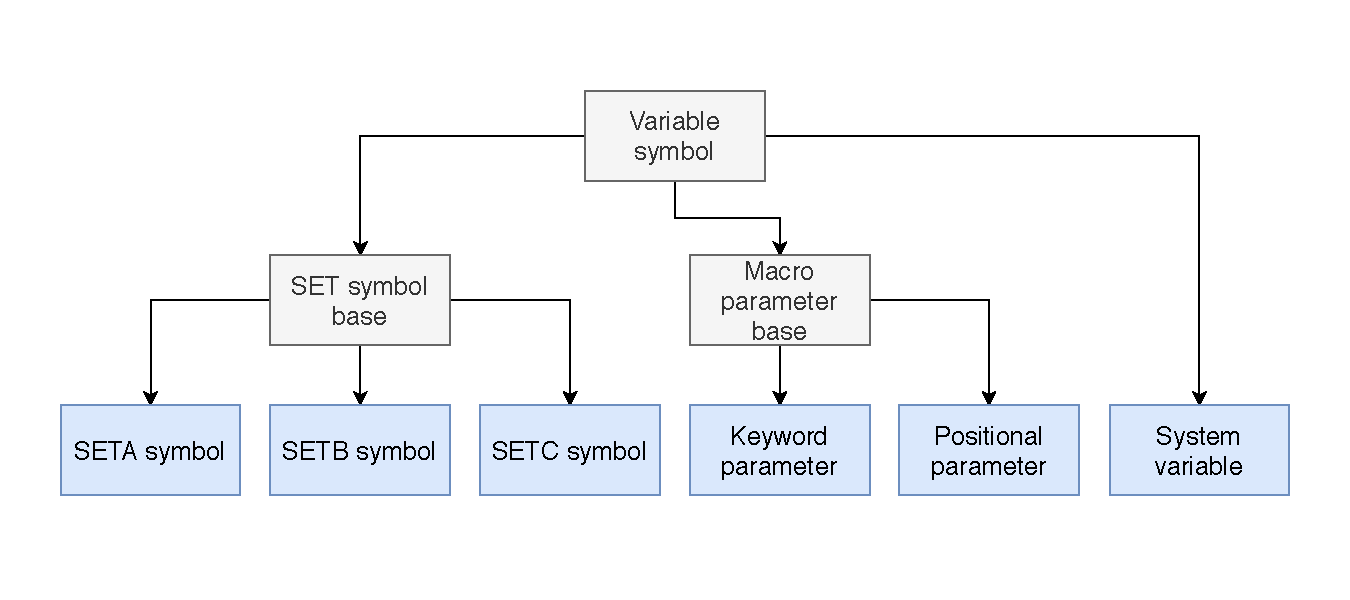
\includegraphics[width=\textwidth]{img/variable_arch}
	\caption{The inheritance of variable symbols.}
	\label{fig06:var}
\end{figure}

\subsectionSrc{LSP context}
{parser\_library/src/context/lsp\_context.h}

The LSP context serves as the collection point for the data needed to answer the LSP requests. It is a part of the HLASM context to be able to pass on the LSP data between different parsed files.

The LSP data collector stores its values inside the LSP context tables. More about the collection of the data and their values can be found in~\cref{lsp_data}.

\subsectionSrc[0.43\linewidth]{Ordinary assembly context}
{parser\_library/src/context/ordinary\_assembly/ordinary\_assembly\_context.h}

The above described structures aimed to describe the high-level part of the language (code generation). As we move closer to the resulting object code of the source file, the describing structures get complicated. Therefore, HLASM context contains object storing just this part of the processing.

\begin{figure}
	\centering
	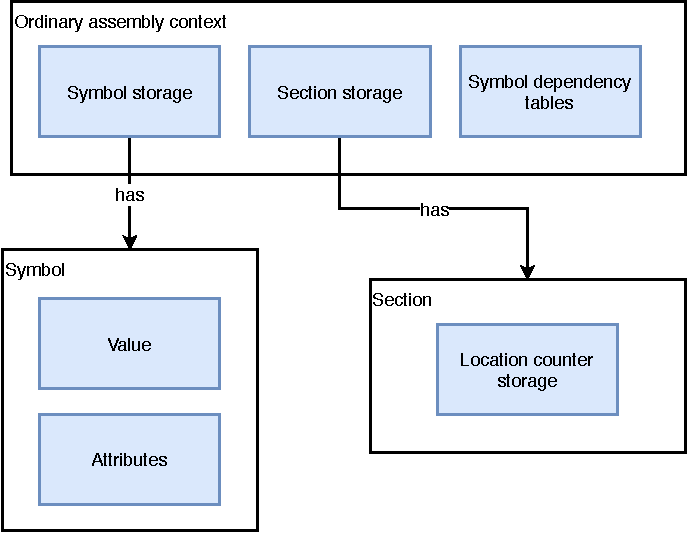
\includegraphics[width=\textwidth]{img/ord_ctx_arch}
	\caption{The composition of ordinary assembly context}
	\label{fig06:ord_ctx}
\end{figure}

Ordinary assembly context consists of three main components (see \cref{fig06:ord_ctx}):
\begin{enumerate}
	\item \emph{Symbol storage}. Stores ordinary symbols (see \cref{ord_sym}).
	\item \emph{Section storage}. Has notion of all generated sections, each section containing its location counters.
	\item \emph{Symbol dependency tables}. Contains yet unresolved dependencies between symbols prior to the currently processed instruction.
\end{enumerate}

\subsubsectionSrc{Symbol}
{parser\_library/src/context/ordinary\_assembly/symbol.h,parser\_library/src/context/ordinary\_assembly/symbol\_attributes.h}

This class represents HLASM ordinary symbol (see \cref{ord_sym}). Besides its identifier and location, symbol contains \emph{value} and \emph{attributes} components.

\begin{description}
	\item[Value] can be assigned \emph{absolute} or \emph{relocatable} values. With addition to that, it can also be assigned an empty value stating that symbol is not yet defined.
	\item[Attributes] structure holds symbol attributes like type, length, scale and integer.
\end{description}

\subsubsectionSrc{Section}
{parser\_library/src/context/ordinary\_assembly/section.h}

Section is a structure representing HLASM section (created by CSECT, DSECT, ...). It contains enumeration \emph{section kind} describing type of the section prior to the used instruction. The structure also holds \emph{location counter storage} with defined location counters.

\subsubsectionSrc{Location counter}
{parser\_library/src/context/ordinary\_assembly/location\_counter.h,parser\_library/src/context/ordinary\_assembly/location\_counter\_data.h,parser\_library/src/context/ordinary\_assembly/address.h}

This structure contains data and operations for one location counter. The data is stored in helper sub-structure \emph{location counter data}.

\begin{description}
	\item[Location counter data] is a structure defining current value of the location counter. It consists of:
	\begin{itemize}
		\item \emph{Storage} stating total number of bytes occupied by the location counter.
		\item Vector of \emph{spaces}, blocks of bytes with yet not known length.
		\item Vector of \emph{storage} between each space.
		\item Currently valid \emph{alignment} (used when data contain spaces).
	\end{itemize}
	
	The location counter value is transformable into a relocatable value. It is represented by structure \emph{address}.
	
	\item[Address] consists of:
	\begin{itemize}
		\item Array of \emph{bases}. A base is a beginning of a corresponding section. They serve as points of reference for the address.
		\item Array of \emph{spaces} that are present in the address. 
		\item \emph{Offset} from the bases.
	\end{itemize}
	
	The common composition of an address is one base section (as the start of the address) and value of storage (as the offset from it).
	
	The need for the whole array of bases to be present is because addresses from different sections can be arbitrarily added or subtracted. This information is needed as the correct sequence of arithmetic operations can reduce number of bases (even spaces) to zero and create absolute value. This value can be later used in places where a relocatable value would be forbidden.
	
	\item[Space] is block of bytes with yet not known length. It is created in the active location counter when execution of counter's operation can not be performed due to non previously defined ordinary symbols. See the different kind of spaces and the reason of creation in  the \cref{tab06:space}.
	
	When a space length becomes known, all addresses containing the spaces need to be updated (remove the space and append offset). Therefore, space structure contains an array of address listeners. Hence, when an address is assigned a relocatable value that contains the space, the address is added to its array. This serves as an easy point of space resolving.
\end{description}



\begin{table}
	\centering
	\begin{tabular}{lr}
		\textbf{Space Kind} &                                          \textbf{Creation} \\ \toprule
		Ordinary            &            when instruction outputs data of unknown length \\
		LOCTR begin         &  when defining more than one location counter in a section \\
		Alignment           &   when current alignment is unknown due to previous spaces \\
		LOCTR set           &     when moving counter's value to the address with spaces \\
		LOCTR max           & when moving counter's value to the next available location \\
		LOCTR unknown       &     when moving counter's value to the yet unknown address \\ \bottomrule
	\end{tabular}
	\caption{Different kinds of spaces and reasons of creation.}
	\label{tab06:space}
\end{table}

ORG instruction can arbitrarily move location counter's value forward and backward. With addition to that, ORG can also order location counter to set it's value to the next available value (the lowest untouched address, see \cref{loctr}). Combining this with the possible spaces creation, location counter holds an array of the location counter data to properly set the next available value.

\subsubsectionSrc{Symbol dependency tables}
{parser\_library/src/context/ordinary\_assembly/symbol\_dependency\_tables.h,parser\_library/src/context/ordinary\_assembly/dependant.h,parser\_library/src/context/ordinary\_assembly/dependable.h}
\label{symbol_dependency_tables}

HLASM forbids cyclic symbol definition. This component maintains dependencies between symbols and detects possible cycles.
Let us describe the main components of dependency resolving.

\begin{description}
	\item[Dependant] is a structure used in the symbol dependency tables. It encapsulates objects that can be dependent on another. Dependant object can be a \emph{symbol}, \emph{symbol attribute} and \emph{space}.
	\item[Dependable] interface is implemented by a class if its instance can contain dependencies. The interface has a method to retrieve a structure holding the respective \emph{dependants}. 
	\item[Resolvable] interface adds up to the dependable interface. It is implemented by objects that serve as values assignable to \emph{depednants}. It provides methods to return \emph{symbol value} with help of the dependency solver. 
	\item[Dependency solver] is an interface that can return value of the symbol providing its identifier. It is implemented by Ordinary assembly context.
\end{description}

\vspace{0.5cm}

Having described building blocks, we can move to the symbol dependency tables composition.
\begin{description}
	\item[Dependency map] is the primary storage of dependencies. It has \emph{dependants} as keys and \emph{resolvables} as values. The semantics for pair \emph{(D,R)} is that D is dependent on the dependencies from R. Each time new dependency is added, this map is searched for cycle.
	
	\item[Dependency sources map] serves as a source objects storage of a resolvable in the dependency map. Hence for the pair \emph{(D,R)} from dependency map, source object of \emph{R} is in the dependency source map under the key \emph{D}. 
	
	The source objects are statements. To be more specific, as one statement can be a source for more distinct resolvables, this source map only stores pointers to the \emph{postponed statements storage}.
	
	\item[Postponed statements storage] holds statements that are sources of resolvables in dependency map. The reason they are stored is that they can not be checked yet as they contain dependencies. Therefore, they are postponed in the storage until all of the dependencies are resolved. Then they are passed to the respective checker.
\end{description}




\chapter{Macro Tracer}
\index{parser\_library!src!debugging@\texttt{debugging}}
\label{macro_tracer}
The macro tracer allows the user to track how the HLASM source code is assembled in experience similar to common debugging tools. The user is able to see step by step how CA instructions are interpreted and how macros are expanded.

This is achieved by implementing the Debug Adapter Protocol. The protocol itself is implemented in the language server component, which uses the macro tracer component.

\section{DAP functionality mapping}

The DAP was originally designed to communicate between an IDE or an editor and a debugger or a debug adapter. For example, when debugging a C++ application in Visual Studio Code, the editor communicates through DAP with a debugger that is attached to a compiled C++ application. Contrary to this, the macro tracer does not run with compiled binary, it only uses the analyzer to simulate the compilation process of high level assembler.

However, even though we are not implementing a real debugger, it makes very good sense to use a debugging interface for tracing the simulation. Parts of the debugging interface that we use in a macro tracer are as follows.
\begin{description}
	\item [Instruction pointer] The instruction pointer is commonly shown in debuggers by highlighting a line of code that is going to be executed next. This is applicable to HLASM without change, since all the instructions are processed one by one in a well-defined order.
	\item [Breakpoints] The user can set a breakpoint when he is interested in tracing only particular section of the code. The compilation simulation will stop when it reaches a line with a breakpoint.
	\item [Continue] The user can restart a paused simulation by using the continue function just as in any debugger.
	\item [Step in and step over] In debuggers, it is possible to use step in / step over functions to debug an implementation of subroutine or to skip it and continue after the application returns from the subroutine. In HLASM, this can be applied to macros and COPY instructions: if the user is interested in what happens inside a macro or a COPY file, he can use step in. Step over skips to the next instruction in the same file.
	\item [Variables] The same way common debuggers show values of runtime variables, the macro tracer uses the same functionality to show values of set symbols, macro parameter values and ordinary symbols. It is also possible to visualize attributes of symbols.
	\item [Call stack] The call stack makes sense with the macro tracer too. It can show the stack of currently processed macros and COPY files. Moreover, macros have local set symbols and parameters, so each stack frame may show a different set of valid variables.
\end{description}
All described functionality (and more) is supported by the DAP. 

%******************************** ARCHITECTURE ************************************  
\sectionSrc{Macro tracer architecture}
{parser\_library/src/debugging/variable.h}

\begin{figure}
	\centering
	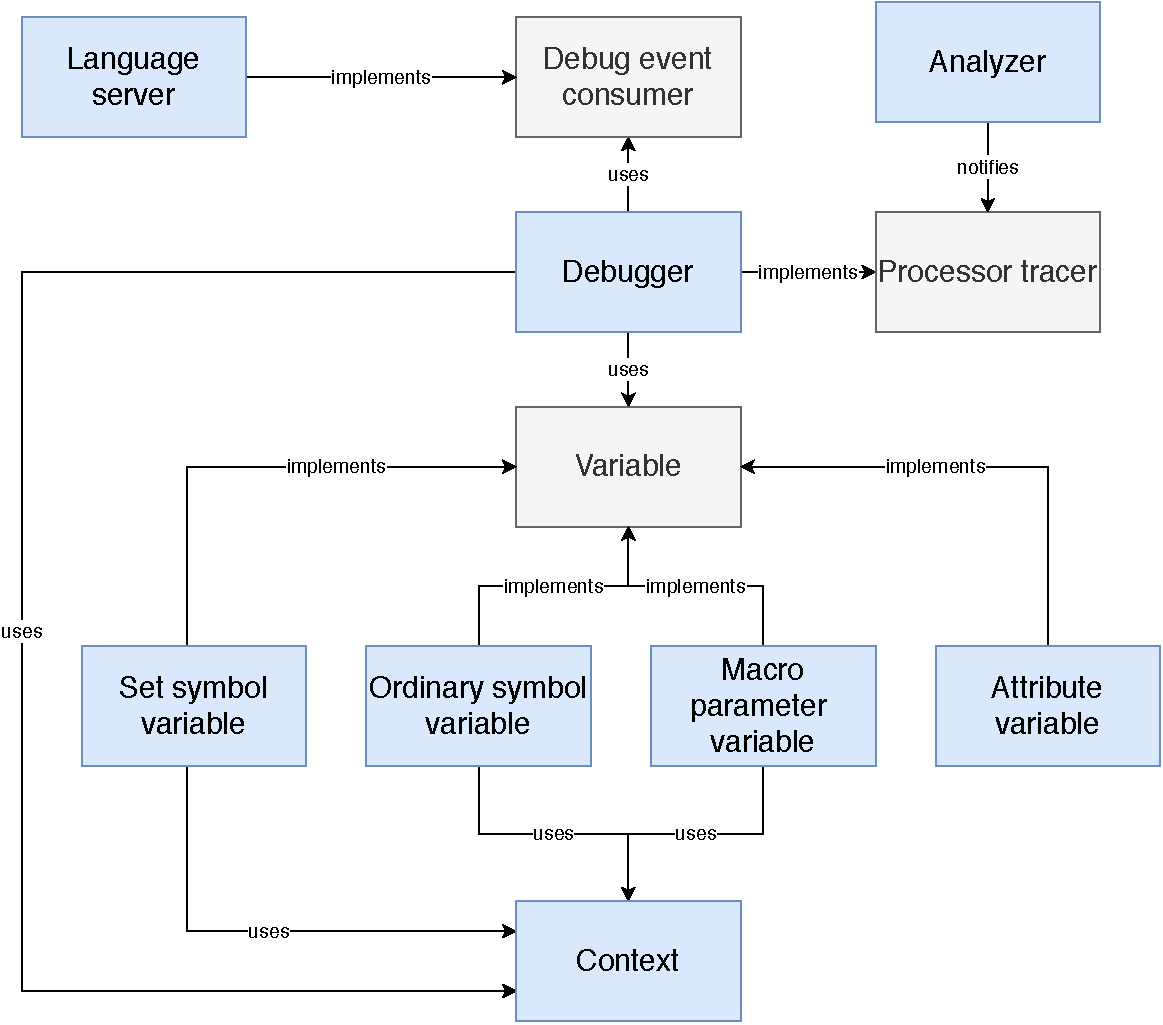
\includegraphics[width=\textwidth]{img/macro_tracer_arch}
	\caption{Architecture of the macro tracer}
	\label{macro_tracer_arch}
\end{figure}

The macro tracer architecture is shown in \cref{macro_tracer_arch}.

\TT{Debugger} is a class that encapsulates all macro tracer functionality. It starts the standard analysis provided by the \TT{analyzer} component in a special thread. The \TT{debugger} implements the \TT{processor\_tracer} interface, which allows it to receive a notification every time a statement is about to be processed.

It is also the \TT{debugger's} responsibility to extract data from the \TT{context} used by the \TT{analyzer} and to transform them into a form compatible with the DAP.

\TT{Debugger} uses an interface \TT{variable} which represents the variable as it is shown to the user --- most importantly, it is a name-value pair. The \TT{variable} interface has four implementations:
\begin{itemize}
	\item \TT{set\_symbol\_variable} \sectionFiles{.53\linewidth}{parser\_library/src/debugging/set\_symbol\_variable.h}
	\item \TT{ordinary\_symbol\_variable} \sectionFiles{.53\linewidth}{parser\_library/src/debugging/ordinary\_symbol\_variable.h}
	\item \TT{macro\_parameter\_variable} \sectionFiles{.53\linewidth}{parser\_library/src/debugging/macro\_param\_variable.h}
	\item \TT{attribute\_variable} \sectionFiles{.53\linewidth}{parser\_library/src/debugging/attribute\_variable.h}
\end{itemize}
First three represent a HLASM symbol of respectable type. They adapt the \TT{context} representation of the symbols to DAP variables.

The \TT{attribute\_variable} represents attributes of all types of symbols. It does not access context, and it is only used by the rest of \TT{variables} to show their attributes.

\sectionSrc[0.45\linewidth]{Debugger}
{parser\_library/src/debugging/debugger.h,parser\_library/src/debugging/debug\_types.h,parser\_library/src/processing/processing\_tracer.h}

The \TT{debugger} component is the core of the macro tracer implementation. When the user starts debugging, the method \TT{launch} is called from the language server component. The \TT{debugger} creates \TT{analyzer} and starts the analysis in a separate thread. The \TT{debugger} implements \TT{processor\_tracer} interface, which only has one method --- \TT{statement}. The \TT{analyzer} calls the \TT{statement} method every time a next statement is about to be processed.

This implementation makes it possible for the \TT{debugger} to stop the analysis using a conditional variable. When it sees fit (e.g. when a breakpoint was hit), the \TT{debugger} can put the thread to sleep and wait for further user interaction. At the same time, it notifies the language server through \TT{debug\_event\_consumer} interface that the analysis has stopped.

There are three important structures in the DAP:
\begin{itemize}
	\item \textbf{Stack frame} Stack frame represents one item in the call stack. Each frame has a name that is shown to the user and points to a line in the source code. In the macro tracer, each frame points either to the next instruction, to a macro call or to a COPY instruction.
	\item \textbf{Scope} Each stack frame may have scopes. A scope is simply a group of variables used to make them organized for the user. The macro tracer uses three scopes: local variables, global variables and ordinary symbols.
	\item \textbf{Variable} Each scope has arbitrary number of variables. Each variable has a name and a value. They may be further structured and may have additional child variables. Therefore, the DAP can be used to present arbitrary tree of variables to the user. \Cref{dap_nested_variables} shows an example regarding nested macro parameters.

\end{itemize}

\begin{listing}
	
	\begin{verbatim}
	MAC (foo,((bar,ex),am),ple,(lorem,ipsum))
	
	1: foo
	2: ((bar,ex),am)
	  1: (bar,ex)
	    1: bar
	    2: ex
	  2: am
	3: ple
	4: (lorem,ipsum)
	  1: lorem
	  2: ipsum
	
	\end{verbatim}
	\caption{An example of how the macro tracer leverages DAP nested variables. First line shows a macro call with a parameter. HLASM treats such parameters as nested arrays. Second part shows how such a parameter is shown in VS Code using nested variables.}
	\label{dap_nested_variables}
\end{listing}

While the thread is stopped, the editor sends requests to display information about the current context. It is the \TT{debugger's} responsibility to extract a list of stack frames from the context, return a list of scopes for each stack frame and a list of variables for each scope. It does not have to deal with the complexity of different types of set symbols and macro parameters, which is done by the implementations of the \TT{variable} interface.



\chapter{VS Code extension}
\label{extension}
The frontend of the project is implemented as an extension to a modern IDE instead of creating a completely new GUI. This approach has the advantage of providing a familiar environment and workflow that the developers are used to.

There are several IDEs that currently (natively) support LSP, such as \emph{Eclipse Che} and \emph{Eclipse IDE}, \emph{vim8}, \emph{Visual Studio} and \emph{Visual Studio Code} and many more. Others, for example \emph{IntelliJ}, have plugins which add the support for LSP.

Our IDE choice is \emph{Visual Studio Code}, due to its popularity and lightweight design. Conveniently, \emph{Theia}, a web-based IDE, supports VSCode extensions, therefore our plugin works with \emph{Theia} as well.

%******************** Standard LSP Extension *************************
\sectionSrc{Standard LSP Extension}
{clients/vscode-hlasmplugin/src/extension.ts,clients/vscode-hlasmplugin/src/serverFactory.ts,clients/vscode-hlasmplugin/src/eventsHandler.ts}
The core of the extension is an activation event which starts the plugin for VSCode.

Upon activation, \emph{Language Client} and \emph{Language server}~\ref{chap:lang_server} are started as child processes of VSCode and a pipe is open for their communication. The LSP communication and its features are handled by the \emph{vscodelc} package. 

To be independent of pipes, we have added an option to use TCP, which assigns a random free port for TCP communication.

%******************** DAP Extension *************************
\sectionSrc{DAP Extension}
{clients/vscode-hlasmplugin/src/debugProvider.ts}


\emph{Macro Tracer}~\ref{macro_tracer} is implemented using DAP, which is also supported out-of-the-box by VSCode. Similarly to LSP TCP support, we dynamically assign a random free port for DAP communication during the activation.

\section{Additional implemented features}

To simplify the work with HLASM in modern editors, several features are added to the extension . These additions are specific for Visual Studio Code (and Theia) and are not a part of the LSP specification.

%******************** Language Detection *************************
\subsectionSrc{Language Detection}
{clients/vscode-hlasmplugin/src/hlasmLanguageDetection.ts}
\label{section:wildcard}
The usual workflow with the extension begins with downloading HLASM source codes from mainframe. Typically, these files will not have any file extension and even if they do, they might differ across various products.

To cope with this problem, there are several mechanisms that help the user to recognize the file as HLASM automatically.

\begin{description}
	\item[Macro Detection] Each file starting with line \emph{MACRO} (arbitrary number of whitespace before and after) is recognized as HLASM.
	\item[Configuration Files Detection] Every file either defined as a program or as a part of a processor group is recognized as HLASM.
	\item[Wildcards] Configuration file \emph{pgm\_conf.json} contains a field \emph{alwaysRecognize}, which consists of user-defined wildcards. Every file that satisfies at least one of these wildcards is recognized as HLASM.
	\item[Automatic Language Detection] Whenever a user opens a file, its contents are scanned line by line. If the file has a sufficient ratio of HLASM lines to all lines, it is considered to be HLASM.
	
	The HLASM line recognition is mostly based on a pre-defined set of most used instructions. If a line correctly uses one of these instructions, it is counted as a HLASM line. Continued line of a HLASM line is also a HLASM line.
	Moreover, a HLASM line must not exceed 80 characters.
	
	Comment lines or empty lines are skipped and not counted. 
	
	We tested the detection on 11.000 HLASM files and 9.000 non HLASM files. The best results were observed using 4/10 ratio, with 88\% true positive recognition and 95\% true negative recognition. 
	
	Because of the indeterminate outcomes, this method is meant to be used as a fall-back in case all previous methods do not suffice.
\end{description}

All detection layers are visualized in \cref{fig08:lang}.

\begin{figure}
	\centering
	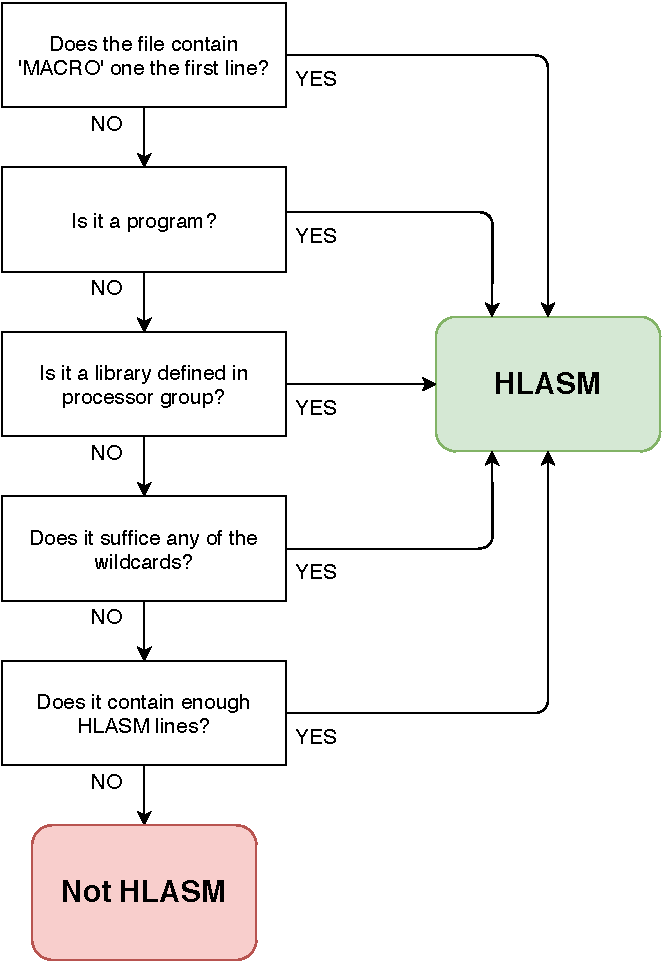
\includegraphics[width=10cm]{img/lang_detection}
	\caption{Language Detection layers.}
	
	\label{fig08:lang}
\end{figure}

%******************** Continuation Handling *************************
\subsectionSrc{Continuation Handling}
{clients/vscode-hlasmplugin/src/continuationHandler.ts,clients/vscode-hlasmplugin/src/customEditorCommands.ts}

Due to historical reasons, HLASM has a 80 character-per-line limitation. Modern languages do not enforce such restriction and therefore IDEs such as VSCode allow the user to extend their lines freely. This causes 2 major inconveniences.

First of all, the user must add the continuation character on a very specific column manually. Secondly, each time the user types in between continuation character and the instruction/parameters, the continuation character is pushed from its requisite position and needs to be moved back, again manually.

To improve this behavior, the extension offers an option to activate \emph{Continuation Handling}. 

The first problem is solved by adding two editor commands \emph{insertContinuation} and \emph{deleteContinuation}, which, when invoked, insert/delete the continuation character on its correct position.

To improve the second problem, the option overrides standard VSCode commands, commonly used when working in editor such as \emph{type}, \emph{deleteLeft}, \emph{deleteRight}, \emph{cut} and \emph{paste}. They offset the continuation character by removing/adding whitespaces in front of it.

%******************** Configuration Prompt *************************
\subsectionSrc{Configuration Prompt}
{clients/vscode-hlasmplugin/src/configurationsHandler.ts}

If a workspace contains a HLASM file, but does not have the configuration files set, the user is prompted to create them. The warning message also offers an option to create templates for them.

%******************** HLASM Semantic Highlighting *************************
\subsectionSrc{HLASM Semantic Highlighting}
{clients/vscode-hlasmplugin/src/semanticHighlighting.ts,clients/vscode-hlasmplugin/src/ASMsemanticHighlighting.ts,clients/vscode-hlasmplugin/src/protocol.semanticHighlighting.ts}

In case of HLASM, a semantic (server-side) highlighting is desired. The multi-layered nature of the language causes that in quite common scenarios, specific parts of the code can be properly highlighted if and only if some previous part was completely processed (parameters for instructions, skipped code thanks to code generation, defined macros, continuations, etc...).

Based on the open pull request to the VSCode Language Server \footnote{https://github.com/microsoft/vscode-languageserver-node/pull/367/files}, we added \emph{semanticHighlighting} as an extra feature of LSP. This feature works in a very similar manner, implementing the LSP interfaces that VSCode provides. It works as a notification from the server to the client, containing ranges inside the document and their respective tokens (e.g. instruction, label, parameter, comment,..). 

On top of that, we extended \emph{semanticHighlighting} to \emph{ASMsemanticHighlighting}, which adds the ability to notify the client about a new code layout, specifically begin, continuation and continue columns. These fields can be set in the HLASM code (via ICTL instruction) and are required for the \emph{Continuation Handling} feature to work properly. Our client-server communication is shown in \cref{fig08:lsp}.


\begin{figure}
	\centering
	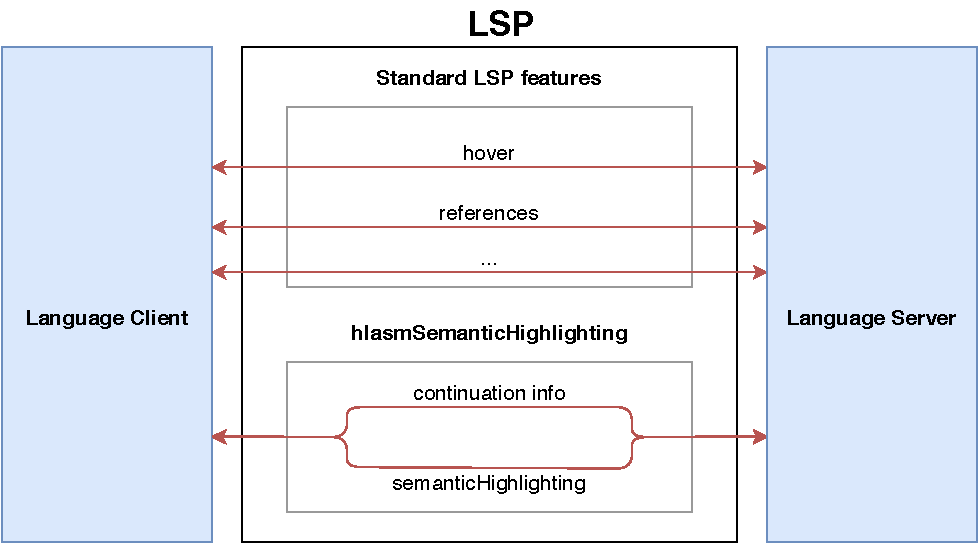
\includegraphics[width=\textwidth]{img/lsp_addition}
	\caption{The addition of semantic highlighting to the LSP communication.}
	
	\label{fig08:lsp}
\end{figure}




\part{Dependencies and build guide}
\chapter{Third party libraries}
\label{3rd_party}
The project uses several third party libraries. Some of them are needed by language server to parse LSP messages and communicate through DAP. Also, we use a third party library to recognize syntax of HLASM.

\begin{description}
	\item [ASIO C++ library]\hspace{-4px}\footnote{\url{https://think-async.com/Asio/}}
	Asio is a cross-platform C++ library for network and low-level I/O programming that provides developers with a consistent asynchronous model using a modern C++ approach. We use it to handle TCP communication in a cross-platform way. Asio implements std::iostream wrappers around the TCP stream, which allows us to abstract from the actual source of the communication.
	
	\item [JSON for Modern C++]\hspace{-4px}\footnote{\url{https://github.com/nlohmann/json}} We use JSON for Modern C++ library to parse and serialize JSON. It is used in both LSP and DAP. It allows us to seamlessly traverse input JSON and extract the interesting values, as well as easily respond with valid JSON messages.
	
	\item [cpp-netlib URI]\hspace{-4px}\footnote{\url{https://github.com/cpp-netlib/uri}} Cpp-netlib URI library is used for parsing URI specified by the RFC3986\footnote{\url{https://tools.ietf.org/html/rfc3986}}, which is used by the LSP and DAP protocols to transfer paths to files. It is the responsibility of the language server to parse the URIs and convert them to file paths, so it is easier to work with them in the parser library. 
\end{description}

\section{Usage of ANTLR4 within the project}
\label{antlr}
We have based part of our analyzer on ANTLR 4 parser generator. ANLTR 4 implements Adaptive $LL(*)$ \cite{parr2014adaptive} parsing strategy.

\subsection{Adaptive $LL(*)$ parsing strategy}
Adaptive $LL(*)$ (or short $ALL(*)$) parsing strategy is a combination of simple, efficient and predictable top-down $LL(k)$ parsing strategy with power of $GLR$ which can handle non-deterministic and ambiguous grammars. 
Authors move the grammar analysis to parse-time. This lets $ALL(*)$ handle any non-left-recursive context-free grammar rules and for efficiency it caches analysis results in lookahead DFA.

Theoretical time complexity can be viewed as a possible downside of $ALL(*)$. Parsing of $n$ symbols takes $O(n^4)$ in theory. In practice, however, $ALL(*)$ seems to outperform other parsers by order of magnitude.

Despite the theoretical $O(n^4)$ time complexity, it appears that the $ALL(*)$ behaves linear on most of the code, with no unpredictable performance or large footprint in practice. In order to support this, authors investigate the parse time vs file size for languages \texttt{C}, \texttt{Verilog}, \texttt{Erlang} and \texttt{Lua} files. They found very strong evidence of linearity on all tested languages (see the original paper for details).

\subsection{ANTLR 4 pipeline}

ANTLR 4, similarly to any other conventional parser generator, processes the inputted code as follows: (1) breaks down the source string into tokens using \textit{lexer} (2) builds parse trees using \textit{parser} . 

This pipeline in ANTLR 4 is broken into following classes: 

\begin{description}
	\item[\texttt{CharStream}] represents input code.
	\item[\texttt{Lexer}] breaks the inputted code into tokens.
	\item[\texttt{Token}] token representation that includes important information like token type, position in code or the actual text.
	\item[\texttt{Parser}] builds parse trees.
	\item[\texttt{TokenStream}] connects the lexer and parser.
\end{description}

\cref{antlr_pipeline} sketches the described pipeline.

\begin{figure}[H]
	\centering
	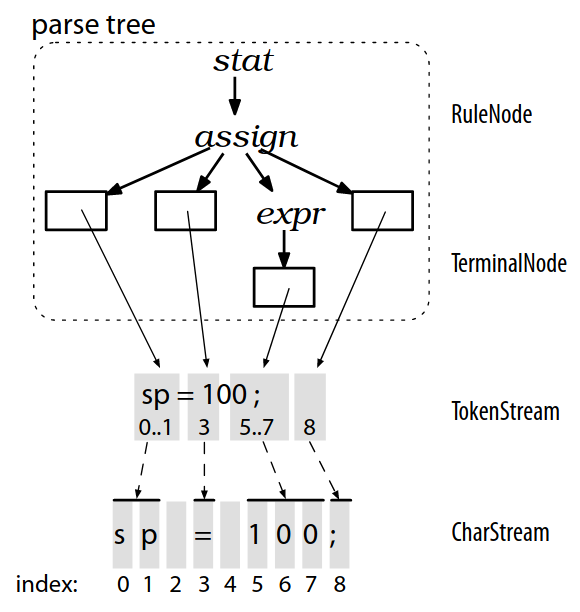
\includegraphics[width=6cm]{img/antlr_pipeline}
	\caption{ANTLR 4 pipeline overview. Taken from \cite{parr2013definitive}.}
	\label{antlr_pipeline}
\end{figure}

\subsection{ANTLR Parser}

The input to ANTLR is a grammar written in antlr-specific language that specifies the syntax of HLASM language (see the 193 grammar rules in the \cref{parser_rules}). The framework takes grammar and generates source code (in C++) for a recognizer, which is able to tell whether input source code is valid or not. Moreover, it is possible to assign a piece of code that executes every time a grammar rule is matched by the recognizer to further process the matched piece of code and produce helper structures (statements).

\subsection{Parse-Tree walking}

ANTLR 4 offers two mechanisms for tree-walking: the parse-tree listeners and parse-tree visitors. The listener can only be used to get a notification for each matched grammar rule. The visitor lets the programmer control the walk by explicitly calling methods to visit children.

We employ the \emph{visitor} approach during evaluation of CA expressions, because we need to have ampler control over the evaluation (such as operator priority).

The ANTLR 4 first generates \texttt{hlasmparserVisitor} and \texttt{hlasmparserBaseVisitor}. The former is an abstract class, the latter is a simple implementation of the former. Both classes define \TT{visit} functions for every grammar rule. A visit function has exactly one argument --- the context of the rule. The simple implementation executes \texttt{visitChildren()}. Our parse-tree visitor --- the \texttt{expression\_evaluator} --- overrides \texttt{hlasmparserBaseVisitor}. In order to evaluate a sub-rule, we call \texttt{visit(ctx->sub\_rule())}, where \texttt{ctx->sub\_rule()} returns the context of the sub-rule. The \texttt{visit()} function matches appropriate function of the visitor based on the context type (for example, \texttt{visit(ctx->sub\_rule())} would call \texttt{visiSub\_rule(..)}).


\chapter{Build instructions}
\label{build}
In this chapter, we describe how to build the project on different platforms. We only describe methods that we use and are guaranteed to work, but other platforms and versions may work as well.

The result of a build is the Visual Studio Code extension packed into a VSIX file, which can be found in the \TT{bin/} subdirectory of the build folder.

\section{Prerequisites}
\label{prereq}
In order to build the project on any platform, following software needs to be installed:

\begin{itemize}
	\item CMake 3.10 or higher
	\item C++ compiler with support for C++17
	\item Java Development Kit (JDK) 8 or higher (the ANTLR project written in Java is built from sources)
	\item Maven (the build system of ANTLR)
	\item Git (needed to download sources of the third party software)
	\item npm (for compiling the typescript parts of the VS Code extension)
\end{itemize}

\section{Windows}

On windows, we use Visual Studio Community 2019. We also have VS configurations for building and testing the project in WSL.

It is also possible to build the project from command line:
\begin{verbatim}
mkdir build && cd build
cmake ../
cmake --build .
\end{verbatim}

\section{Linux}

In addition to the prerequisites listed in \cref{prereq}, linux build has two more prerequisites:

\begin{itemize}
	\item pkg-config
	\item UUID library
\end{itemize}


We build the project for Ubuntu 18.04 and for the Alpine linux.
\subsection{Ubuntu}
On Ubuntu 18.04 the following commands install all prerequisites and then build the project into \TT{build} folder:

\begin{verbatim}
apt update && sudo apt install cmake g++-8 uuid-dev npm default-jdk
                       pkg-config maven git
mkdir build && cd build
cmake -DCMAKE_C_COMPILER=gcc-8 -DCMAKE_CXX_COMPILER=g++-8 ../
cmake --build .
\end{verbatim}


\subsection{Alpine linux}

The build works on Alpine linux version 3.10. The following commands install all prerequisites and then build the project into \TT{build} folder:
\begin{verbatim}
apk update && apk add linux-headers git g++ cmake util-linux-dev npm
                      pkgconfig openjdk8 maven
mkdir build && cd build
cmake ../
cmake --build .
\end{verbatim}


\section{Mac OS}
We have only built the project on MacOS 10.14. In order to successfully build, we require LLVM 8 (it can be installed by using homebrew).

The project can be built with a snippet like this:
\begin{verbatim}
mkdir build && cd build
cmake -DCMAKE_C_COMPILER=clang -DCMAKE_CXX_COMPILER=clang++
      -DLLVM_PATH=<path-to-llvm-installation> ../
cmake --build .
\end{verbatim}
For instance, a possible path to LLVM is \TT{/usr/local/opt/llvm\@8}

\section{Running tests}
Once the project is built, there are two test executables in the \TT{bin/} subdirectory of the build folder: \TT{library\_test} and \TT{server\_test}. Just run both of them to verify the build. The tests must be run from the \TT{bin} folder, because they need to load resources from the \TT{bin/test/} directory.

\section{Installation}
The built VSIX can be manually installed into VS Code by following these steps:
\begin{enumerate}
	\item Open the extensions tab (Ctrl + Shift + X)
	\item Select ``More actions ...'' (the $\cdots$ icon)
	\item Select ``Install from VSIX...''
	\item Find the VSIX file and confirm the selection.
	\item The plugin is now installed.
\end{enumerate}

Alternatively, the plugin can be installed with the following command:
\begin{verbatim}
code --install-extension <path-to-vsix>
\end{verbatim}



\bibliography{biblio} 
\bibliographystyle{apalike}

\printindex
\begin{appendices}


\begin{foldoutfloat}
	\chapter{Architecture of the project}
	\label{all_arch}
	\thispagestyle{empty}

	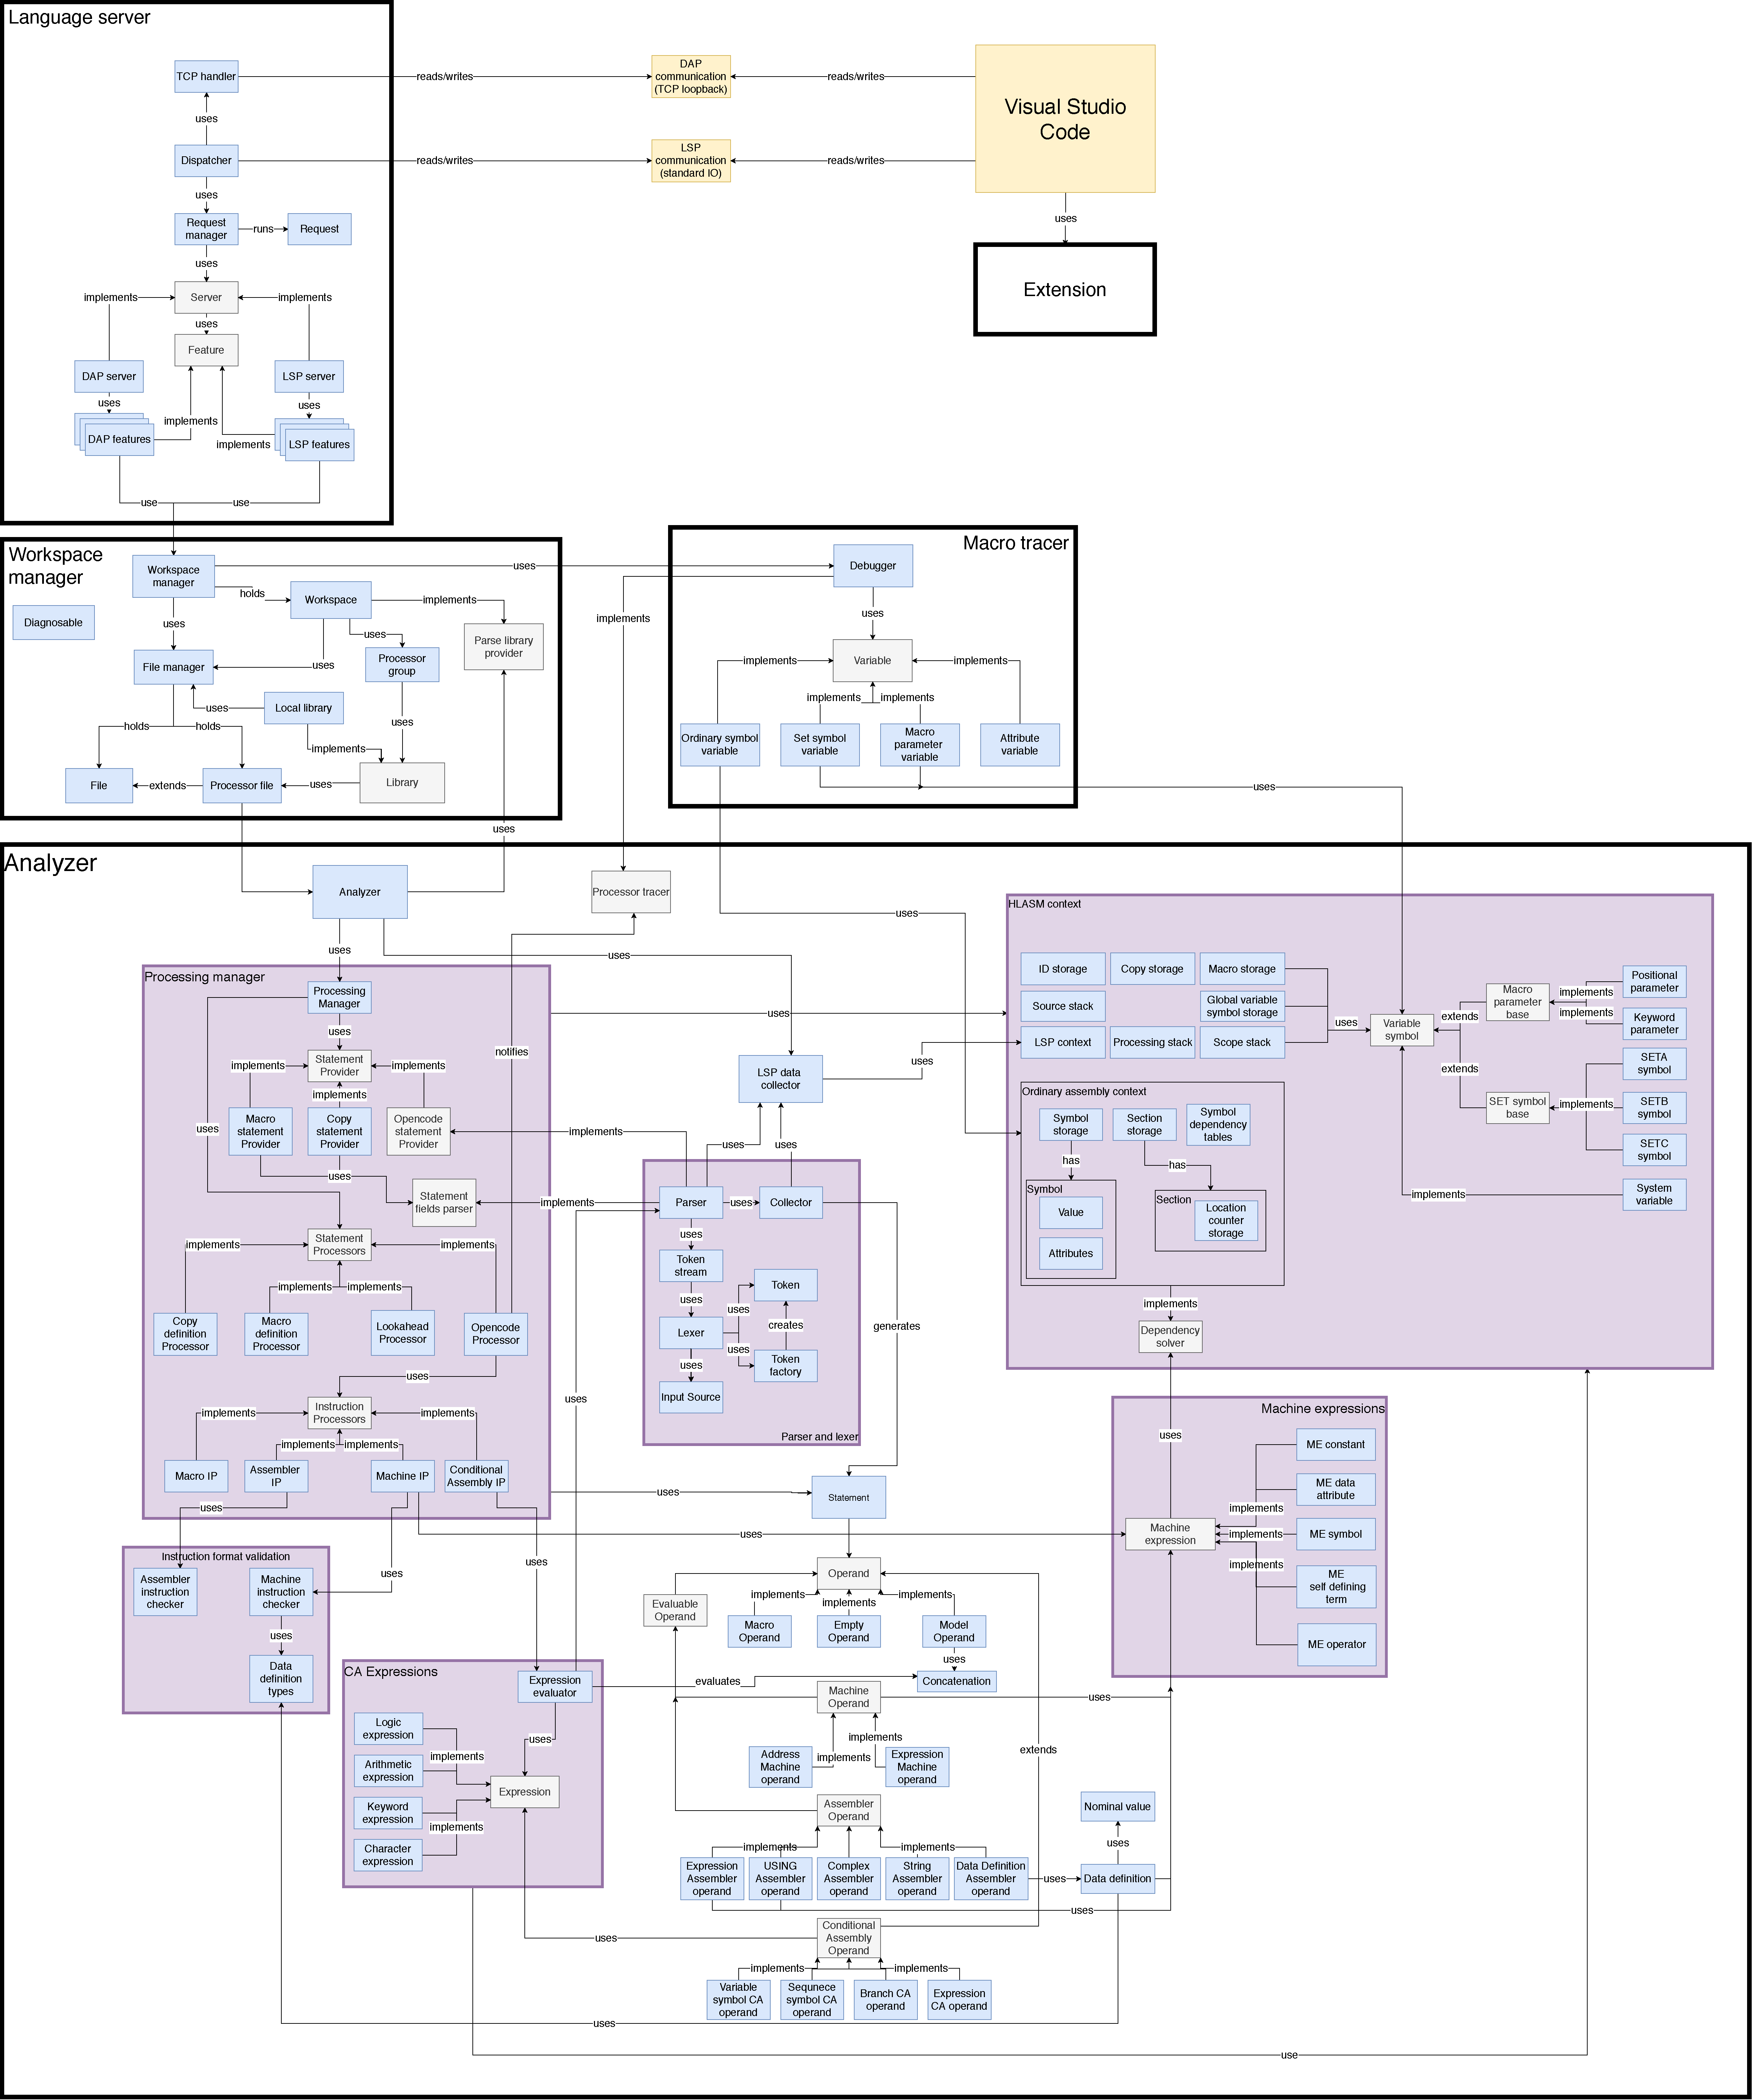
\includegraphics[width=35cm]{img/all_arch}
	\caption{Architecture of the whole project}
\end{foldoutfloat}

\begin{foldoutfloatlandscape}
	\chapter{Parser grammar}
	\label{parser_rules}
	\thispagestyle{empty}
	
	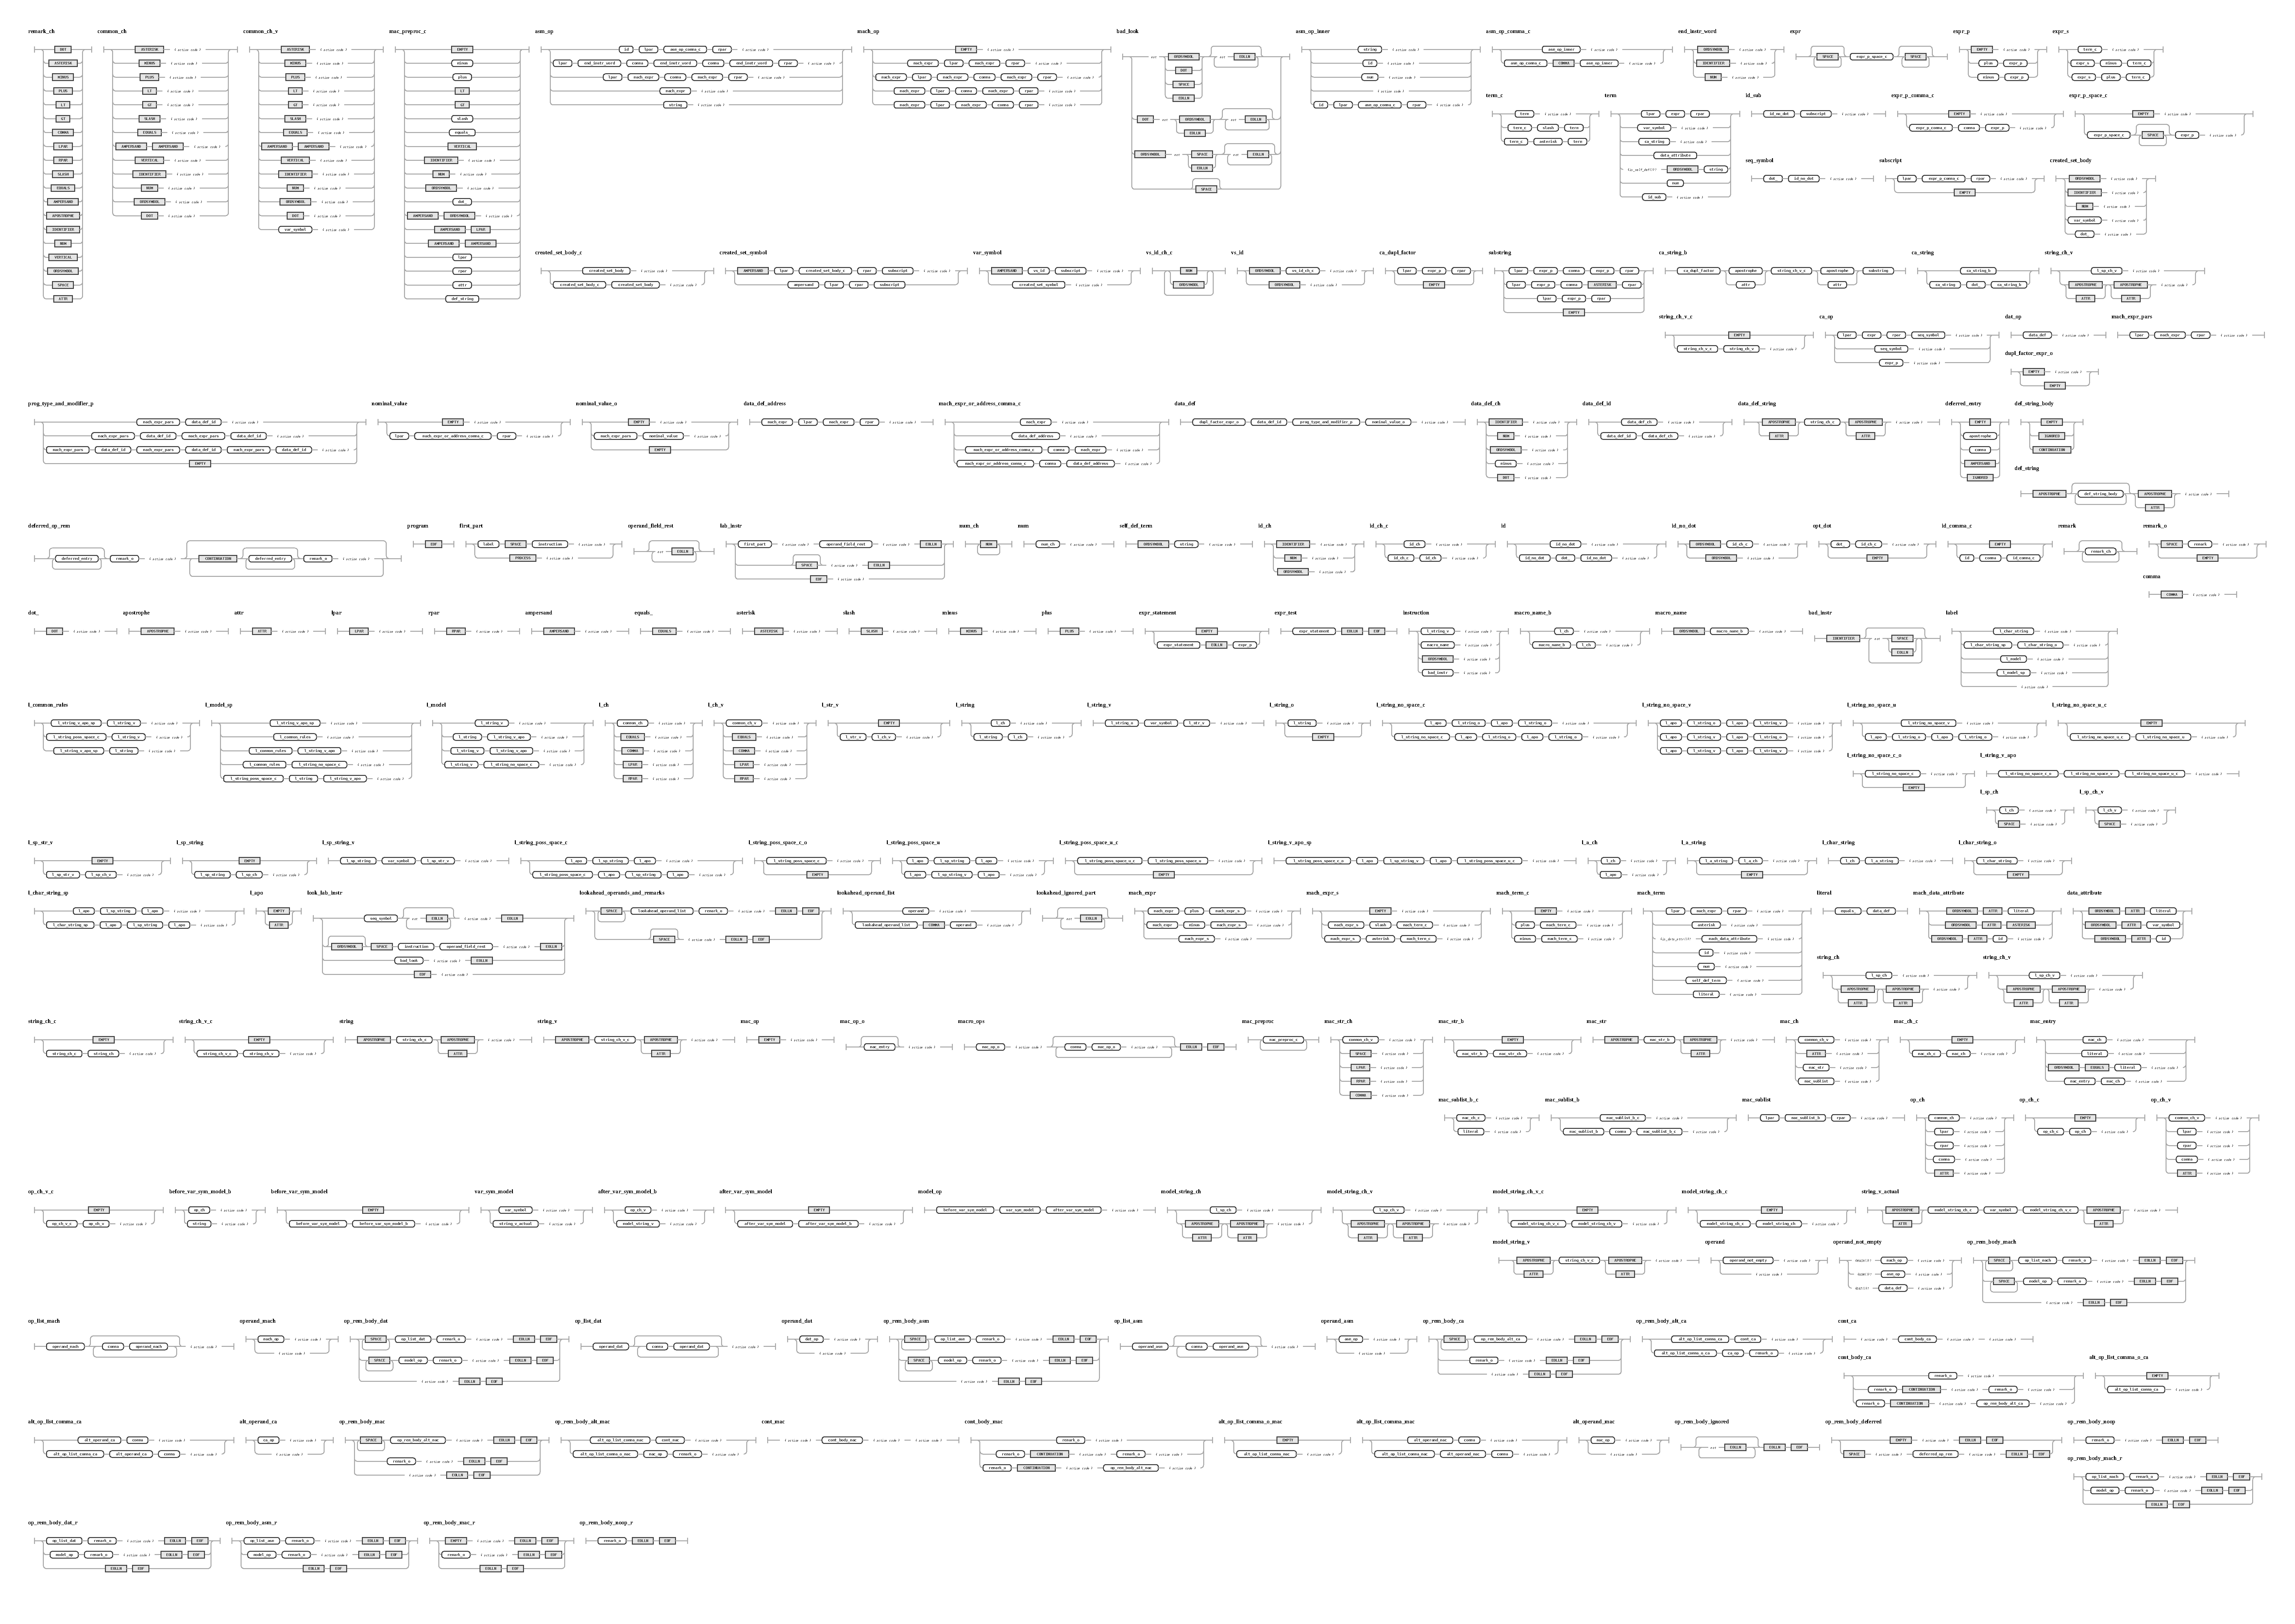
\includegraphics[width=45cm]{img/grammar}
	\caption{All 193 grammar rules}
\end{foldoutfloatlandscape}



\end{appendices}

\end{document}
